\chapter{Experimental study} \label{Experimental Studies}


The experimental study was conducted to replicate and complement the results of the corpus study. In contrast to the corpus study, the experimental study did not investigate natural, \isi{conversational speech} but \isi{read speech}. As thoroughly discussed in Chapter \ref{General Method}, this has the advantage of including a great number of types and tokens and investigating durational properties of words under controlled conditions.

 The data was collected in two experiments carried out in October 2015 and October 2016 at the University of Cambridge's Phonetic Laboratory. While in the first experiment the \is{un-}\prefix{un} and \is{in-}\prefix{in}data was collected, the second experiment was conducted to record the \is{dis-}\prefix{dis} and \is{-ly}\suffix{ly}-data. 
  The set-up of both experiments was identical. The experiments consisted of two parts, a reading task and a decomposability rating. 
 Both experimental tasks will be described in detail in the first section of this chapter.
 The data was analyzed with regard to two aspects, \isi{decomposability} and duration. First, I will describe the \isi{decomposability} analysis.  Then, I will lay out the durational analyses and their results. At the end of the chapter, I will summarize the results. A thorough discussion of the results and their theoretical implications will be conducted alongside with the results from the corpus study in Chapter \ref{Conclusion}.



\section{Methodology}


\subsection{Stimuli} \label{stimuli experiment}

% investigated strutuctues
 Five different structures were investigated in the experimental studies. The structures and their environments are shown in \tabref{tbl:overview structures environment experiment repetition}. For each of the investigated affixes, the included environments and examples are listed (see \sectref{experiment data composition} for a detailed description of the investigated structures and environments). In contrast to the corpus study, the experimental study did not only investigate the allomorph \is{im-}/ɪm/  for the prefix \is{in-}\prefix{in}, but also /ɪn/. Note that no distinction between locative and \is{negative in-}negative \prefix{in} is made in the table but that this distinction was taken into consideration when selecting the experimental items, as well as when analyzing the data.



\begin{table*}
	
	\caption{Overview of the investigated structures in the experimental study}
	\label{tbl:overview structures environment experiment repetition}
					
	
	\resizebox{\textwidth}{!}{%
		\begin{tabular}{ccccc} 
		\lsptoprule
		
			& \begin{tabular}[c]{@{}c@{}} Phonological double\\ in complex word\end{tabular}                           &  \begin{tabular}[c]{@{}c@{}}Singleton\\ in complex word\end{tabular}                                                   & \begin{tabular}[c]{@{}c@{}}Singleton \\ in base\end{tabular}               &
			\begin{tabular}[c]{@{}c@{}}Orthographic double\\ in simplex word\end{tabular} \\
			\midrule
			%\\
			
			\{\isi{un-}\}  & 
			{\begin{tabular}[c]{@{}c@{}} \textit{unnatural}\\ (n\#nV)\end{tabular}}         & {\begin{tabular}[c]{@{}c@{}} \textit{uneven \phantom{space} untold} \\ (n\#V)\phantom{space }(n\#C)\end{tabular}}                               & {\begin{tabular}[c]{@{}c@{}} \textit{natural}\\ (\#nV)\end{tabular}  } &
			NA                                                                            
			\\
			\\
			
			\{\isi{in-}\}  & 
			{\begin{tabular}[c]{@{}c@{}} \textit{immortal}\\ (m\#mV)\\  \textit{innumerous}\\ (n\#nV)\end{tabular}} & 
			 {\begin{tabular}[c]{@{}c@{}}\phantom{spa} NA \phantom{spa}  \textit{impossible}\\ \phantom{more space } (m\#C)\\  \textit{inefficient \phantom{sp}   intolerant}\\ (n\#V)\phantom{space } (n\#C)\end{tabular}} & {\begin{tabular}[c]{@{}c@{}} \textit{mortal}\\ (\#mV)\\  \textit{numerous}\\ (\#nV)\end{tabular}} &
			 NA                                                                            \\
			\\
			
			\{\isi{dis-}\} & 
			{\begin{tabular}[c]{@{}c@{}} \textit{dissatisfy}\\ (s\#sV)\end{tabular}}                      &
			
			{\begin{tabular}[c]{@{}c@{}} \textit{disarm \phantom{space} } \color{black} NA\\ (s\#V)\phantom{space} \phantom{s\#V} \end{tabular}}                   & {\begin{tabular}[c]{@{}c@{}} \textit{satisfy}\\ (\#sV)\end{tabular}}        &
			{\begin{tabular}[c]{@{}c@{}} \textit{dissertation}\\ (sV)\end{tabular}}                     \\
			\\
			
			\{\isi{-ly}\}  & 
			{\begin{tabular}[c]{@{}c@{}} \textit{really}\\ (Vl\#l)\end{tabular}}                           & 
			{\begin{tabular}[c]{@{}c@{}} \textit{truly \phantom{spaceee}} \color{black} NA\\ (V\#l)\phantom{space }\phantom{V\#C}\end{tabular}}                 & {\begin{tabular}[c]{@{}c@{}} \textit{real}\\ (Vl\#)\end{tabular}}      &
			{\begin{tabular}[c]{@{}c@{}} \textit{belly}\\ (Vl)\end{tabular}}                                
			
			\\	\lspbottomrule
		\end{tabular}%
		
	}
	

\end{table*}


The experimental stimuli were selected from a word list that features all words with the desired structures attested in \is{Corpus of Contemporary American English (COCA)} {COCA} (\citealt{Davies.20082014}). This list was generated using the speech corpus management system Coquery (\citealt{Kunter.2016}). The selection of stimuli was then guided by several criteria. 
The first criterion was that only types which are attested in the \textit{OED} (\citealt{OED.2013}) were considered to serve as stimuli in the experiments. 
The second criterion concerns morphological structure. All complex stimuli in the experiments had to feature different roots.\footnote{As in the corpus study, morphological structure was coded by using the criteria described in \sectref{theory:in}.} For example, since the two derivatives \textit{unnatural} and \textit{unnaturally} feature the same root, i.e. \{nature\}, only one of them was included in the study. Complex words with fewer morphemes were preferred over complex words with more morphemes, e.g. the word \textit{unnatural} was preferred over the word \textit{unnaturally}. 
 The third criterion concerns \isi{word form frequency}. For each environment, types of different \is{frequency}frequencies were selected, i.e. the same number of types with low, mid and high \isi{frequency} were selected. A low \isi{frequency} word was defined to have a \isi{frequency} lower than 10, a mid \isi{frequency} word was defined to have a \isi{frequency} between 10 and 100, and a high \isi{frequency} word was defined to have a \isi{frequency} higher than 100. Frequency measures were taken from \is{Corpus of Contemporary American English (COCA)} {COCA} (\citealt{Davies.20082014}).
  The fourth criterion concerns prosodic structure. When possible, the number of syllables and the \isi{stress} pattern of the stimuli was kept similar across the environments of each affix. In other words, the distribution of \isi{stress} and syllable number in a particular environment should not be unique to that environment. To test whether the prosodic structure of the stimuli differed significantly between the environments of a particular affix, Wilcoxon Signed-Rank tests (see, for example, \citealt[Chapter 5]{Crawley.2012}) were applied. In case prosodic features differed significantly, additional stimuli were added until there was no significant difference between environments.
 
 %affix-specific criteria
 In addition to the four criteria just mentioned, which applied to all stimuli, some criteria only applied to words with specific affixes. 
 For \is{dis-}\prefix{dis}, only words featuring voiceless /s/ were included in the study. 
  For \is{in-}\prefix{in} and \is{dis-}\prefix{dis}, when possible, the same number of \is{semantic transparency}semantically transparent and opaque words was included for each environment. Since \is{un-}\prefix{un} and \is{-ly}\suffix{ly}-affixed words do not show variation in \isi{semantic transparency} (see \sectref{The decomposability of the four affixes: a comparison} for discussion), this criterion was irrelevant for these data sets.
 Furthermore, when possible, the same number of derivatives with negative and \is{locative in-}locative \prefix{in} was included for each of the \is{in-}\prefix{in}environments. 
 
 

 %application of criteria
The application of the selection criteria led to different numbers of included stimuli for each affix and each environment. 
There are two reasons for these differences. The first reason is that for some environments only few types are attested, i.e. the number of included stimuli is restricted by the number of existing types. The second reason is methodological in nature. 
In some environments 
certain features, for example, base-initial \isi{stress} and high \isi{word form frequency}, tend to appear together. This raises the problem that certain effects cannot be tested independently from each other. To alleviate the problem, i.e. to ensure the independence of effects, it was sometimes necessary to add more stimuli with a certain combination of features to an environment. As a result, for some environments more stimuli were included than for others. 
In the following, I will discuss the stimuli selection for each affix. In these discussions, I will also point out for which environments the selection criteria were not, or only partially, met.\footnote{A list of all experimental stimuli can be found in \hyperref[Appendix E: Stimuli of Experimental Study]{Appendix E}.} 


\subsubsection{\textit{un-}}

\tabref{tbl:distribution of un types in experiment} shows the distribution of  stimuli in the \is{un-}\prefix{un}data set across environments. 
%Doubles for the prefixes
22  \is{un-}\prefix{un}prefixed stimuli with a phonological double ({n\#nV}) were included. These 22 stimuli represent all \is{un-}\prefix{un}prefixed types with a phonological double and different roots attested in \is{Corpus of Contemporary American English (COCA)} {COCA} (\citealt{Davies.20082014}) and the \textit{OED} (\citealt{OED.2013}). 
Due to the small number of available types, only the first two selection criteria (attestation in the \textit{OED} (\citealt{OED.2013}) and different roots) were taken into account when selecting these stimuli. Considering the other selection criteria would have resulted in a fatal decrease of available stimuli. 



The number of stimuli with singleton environments in complex words (n\#C and n\#V) roughly matches the number of stimuli with a double consonant. 21 types with a  singleton followed by a consonant ({n\#C}), and 26 types with a singleton followed by a vowel ({n\#V}) were included. 
Of the 21 \is{un-}\prefix{un}prefixed words with a following consonant, seven were of high, seven of mid, and seven were of low \isi{frequency}.
For the following-vowel words, eight items were of low \isi{frequency}, eight of mid \isi{frequency} and 10 of high \isi{frequency}. The reason for including more stimuli of high \isi{frequency} was due to the distribution of prosodic structure across the environments. To make the prosodic structure of \is{un-}\prefix{un}prefixed words with a singleton comparable to the one of \is{un-}\prefix{un}prefixed words with a double consonant, some additional words with a specific prosodic structure needed to be added to the data set. These words were of high \isi{frequency}.




%Base words
The selection of the base words ({\#nV}) was determined by the selection of words with a phonological double, i.e.  for each word with a phonological double the pertinent base word was included in the experiment. Two base words were not included in the study due to a mistake in the experimental set-up. 




%Overview table

\begin{table}
	\caption{Distribution of  \textit{un}-types in experimental study}
	\label{tbl:distribution of un types in experiment}

	
		\begin{tabular} {llr}
\lsptoprule
			Environment & Example & Number of  Types\\

			\midrule
			n\#nV&\textit{unnatural} & 22\\ 
			n\#C& \textit{untold} & 21\\ 
			n\#V& \textit{uneven} & 26 \\
			\#nV& \textit{natural} & 20 \\ 
			\midrule
			Total&  & 89 \\ 
			\lspbottomrule                                                                                
		\end{tabular}
		

	
\end{table}



\subsubsection{\textit{in-}}

\tabref{tbl:distribution of in types in experiment} shows the distribution of  stimuli in the /ɪn/-data set across environments. 
Four stimuli with a phonological double ({n\#nV}) were included. As with \is{un-}\prefix{un}, these four stimuli represent all /ɪn/-prefixed types with a phonological double and different roots attested in \is{Corpus of Contemporary American English (COCA)} {COCA} (\citealt{Davies.20082014}) and the \textit{OED} (\citealt{OED.2013}). Only the first two selection criteria (attestation in the \textit{OED} (\citealt{OED.2013}) and different roots) were taken into account when selecting these stimuli. 



Only 19 /ɪn/-prefixed types with a following /t/ ({n\#C}) were attested  in \is{Corpus of Contemporary American English (COCA)} {COCA} (\citealt{Davies.20082014}) and the \textit{OED} (\citealt{OED.2013}).  Eight of them feature \is{locative in-}locative \prefix{in} and 11 \is{negative in-}negative \prefix{in}. All of them were included in the study irrespective of their \is{frequency}frequencies, \isi{semantic transparency} and prosodic structure. 

For /ɪn/ followed by a vowel ({n\#V}), only three types with \is{locative in-}locative \prefix{in} were attested. All three types were included irrespective of their \isi{frequency}, \isi{semantic transparency} and prosodic structure. 
To keep the number of stimuli comparable across affixes, and to account for the lack of \is{locative in-}locative \prefix{in}prefixed words, 24 \is{negative in-}negative \prefix{in}prefixed types with a singleton followed by a vowel were included. They are equally distributed among the three \isi{frequency} categories.  



%Base words
Three base words with a singleton /n/ ({\#nV}) were included. The selection was determined by the selection of words with a phonological double ({n\#nV}). The base of one of the four /ɪn/-prefixed words with a phonological double is bound and was therefore not included. 
The prosodic structure of /ɪn/-prefixed words is comparable across environments.


\begin{table}
	\caption{Distribution of /ɪn/-types in experimental study}
	\label{tbl:distribution of in  types in experiment}

	
		\begin{tabular} {llr}
\lsptoprule
			Environment & Example & Number of  Types\\

			\midrule
			n\#nV&\textit{innumerous} & 4 \\ 

			n\#C&\textit{intolerant} & 19 \\ 
						n\#V&\textit{inefficient} & 27 \\ 
			\#nV&\textit{numerous} & 3\\ 
			\midrule   
			Total&  & 83 \\ 
			\lspbottomrule                                                                                
		\end{tabular}
		%		\vspace*{-0.5cm}
	
\end{table}


\subsubsection{\textit{im-}}

%Doubles for the prefixes
\tabref{tbl:distribution of im types in experiment} shows the distribution of  stimuli in the \is{im-}/ɪm/ -data set across environments. 19 stimuli with a phonological double ({m\#mV}) were included. These are all \is{im-}/ɪm/ -prefixed types with a phonological double and different roots attested in \is{Corpus of Contemporary American English (COCA)} {COCA} (\citealt{Davies.20082014}) and the \textit{OED} (\citealt{OED.2013}). As with \is{un-}\prefix{un} and /ɪn/, only the first two selection criteria (attestation in the \textit{OED} (\citealt{OED.2013}) and different roots) were taken into account when selecting these stimuli.


28 complex stimuli with a singleton ({m\#C}) were included in the study. Only eight of these stimuli feature \is{locative in-}locative \prefix{in}. These eight are the only types with a singleton /m/ and \is{locative in-}locative \prefix{in} attested in \is{Corpus of Contemporary American English (COCA)} {COCA} (\citealt{Davies.20082014}) and the \textit{OED} (\citealt{OED.2013}). Two of them are of low \isi{frequency}, and six of them are of high \isi{frequency}.
 To account for the uneven distribution of \isi{frequency} with \is{locative in-}locative \prefix{in}, eight of the 20 included \is{negative in-}negative \prefix{in}items are of mid \isi{frequency} (six are of low and six are of high \isi{frequency}).


%Base words
For 17 of the 19 stimuli with a phonological double, the pertinent base word ({\#mV}) was included in the experiment. Two stimuli with a phonological double feature bound roots as bases. Their bases were therefore not included as stimuli. The prosodic structure of \is{im-}/ɪm/ -prefixed words is comparable across environments.



\begin{table}

	\caption{Distribution of /ɪm/-types in experimental study}
	\label{tbl:distribution of im types in experiment}

	
		\begin{tabular} {llr}
\lsptoprule

Environment &Example &Number of   Types\\

 \midrule
 m\#mV&\textit{immortal} & 19  \\
  m\#C&\textit{impossible} & 28 \\
  \#mV&\textit{mortal} & 17 \\
 \midrule
 Total& & 64\\
 \lspbottomrule                                                                                
		\end{tabular}
			%\vspace*{-0.5cm}
	
\end{table}



\subsubsection{\textit{dis-}} \label{dis stimui}

\tabref{tbl:distribution of dis types in experiment} shows the distribution of  stimuli in the \is{dis-}\prefix{dis}data set across environments. 
15 \is{dis-}\prefix{dis} stimuli with a phonological double (s\#sV) were included. As with the other prefixes, these stimuli represent all types with a phonological double and different roots attested in \is{Corpus of Contemporary American English (COCA)} {COCA} (\citealt{Davies.20082014}) and the \textit{OED} (\citealt{OED.2013}),  and only the first two selection criteria (attestation in the \textit{OED} (\citealt{OED.2013}) and different roots) were taken into account when selecting these stimuli. 

%dis
30 complex stimuli with a singleton (s\#V) were included. They are equally distributed among the different \isi{frequency} ranges, i.e. 10 words are of high \isi{frequency}, 10 are of mid \isi{frequency} and 10 are of low \isi{frequency}. 
Only two of the \is{dis-}\prefix{dis}prefixed stimuli with a phonological singleton are semantically opaque. 


%Base words
The selection of the base words (\#sV) was determined by the selection of words with a phonological double. 
Nine bases were included. Six bases are bound and were therefore not included. 

%Orthographic Doubles
Five simplex words with orthographic doubles (sV) were included. These were the only types attested in \is{Corpus of Contemporary American English (COCA)} {COCA} (\citealt{Davies.20082014}) and the \textit{OED} (\citealt{OED.2013}). 
All of them were included irrespective of their \isi{frequency} and their prosodic structure. 

With regard to prosodic structure, it should be noted that double consonant words and base words significantly differ from words featuring a singleton in that double consonant words and base words bear base-initial \isi{stress} whereas words with a singleton often do not. Due to the lack of double consonant words and base words without base-initial \isi{stress}, as well as the lack of singleton words with base-initial \isi{stress}, it was impossible to even out this bias in the distribution of \isi{stress}.


\begin{table}[h!]
	\caption{Distribution of \textit{dis}-types in experimental study}
	\label{tbl:distribution of dis types in experiment}

	
		\begin{tabular} {llr}
\lsptoprule
			Environment & Example & Number of  Types\\

			\midrule
			s\#sV&\textit{dissatisfy} & 15 \\ 
			s\#V&\textit{disarm} & 30\\ 
			\#sV&\textit{satisfy} & 9\\ 
			sV&\textit{dissertation} & 5 \\ 
			\midrule   	
			Total&  & 59\\ 
			\lspbottomrule                                                                                
		\end{tabular}
				%	\vspace*{-0.5cm}
	
\end{table}



\subsubsection{\textit{-ly}} \label{stimuli ly}
%Overview table


\begin{table}[b]
	\caption{Distribution of \textit{-ly}-types in experimental study}
	\label{tbl:distribution of ly types in experiment}
	
	
		\begin{tabular} {llr}
\lsptoprule			
			Environment & Example & Number of  Types\\
			\midrule
			Vl\#l &\textit{really} & 31 \\ 
			V\#l &\textit{truly} & 30 \\ 
			Vl\# &\textit{real} & 31\\ 
			Vl &\textit{belly} & 11\\ 
			\midrule   	
			Total&  & 103 \\ 
			\lspbottomrule                                                                                
		\end{tabular}
		%\vspace*{-0.5cm}
	
\end{table}




\tabref{tbl:distribution of ly types in experiment} shows the distribution of  stimuli in the \is{-ly}\suffix{ly}-data set across environments. 
31 stimuli with a phonological double (Vl\#l) were included. 
They are of four different types. These four types differ with regard to their \isi{orthography} and with regard to whether \is{-ly}\suffix{ly} is preceded by an additional suffix. The four types are shown with examples in \tabref{tbl:The four types of ly-stimuli with a phonological double}.\pagebreak

\begin{table}
	\caption{The four types of \textit{-ly}-stimuli with a phonological double\label{tbl:The four types of ly-stimuli with a phonological double}}
		\begin{tabular} {llr}
\lsptoprule
			Type & Example & Number of  Stimuli\\
			\midrule
			$\langle$-lly$\rangle$&\textit{really} & 5 \\ 
			$\langle$-lely$\rangle$  \phantom{hggzujg}&\textit{solely} & 8\\ 
			$\langle$-ally$\rangle$&\textit{educationally} &9\\ 
			$\langle$-fully$\rangle$&\textit{successfully} & 9 \\ 
			\lspbottomrule                                                                                
		\end{tabular}
\end{table}


The first type are complex words ending in the orthographic string $\langle$lly$\rangle$ with no other suffix preceding \is{-ly}\suffix{ly} (e.g. \textit{really}). These words are extremely rare. Only five types are attested  in \is{Corpus of Contemporary American English (COCA)} {COCA} (\citealt{Davies.20082014}) and the \textit{OED} (\citealt{OED.2013}). All were included. None of them is of high \isi{frequency}.

The second type of double consonant stimuli are complex words ending in the orthographic string $\langle$lely$\rangle$ (e.g. \textit{solely}). These words are also quite rare, i.e. only eight  types are attested and were included as stimuli. Three of them  are of low \isi{frequency}, two are of mid \isi{frequency} and two are of high \isi{frequency}.



Most of the \is{-ly}\suffix{ly}-words with a double consonant are preceded by either the suffix \suffix{al} (e.g. \textit{educationally}), i.e. the third type of \is{-ly}\suffix{ly}-stimuli with a phonological double, or by the suffix \suffix{ful} (e.g. \textit{successfully}), i.e. the fourth type of \is{-ly}\suffix{ly}-stimuli with a phonological double. Nine types of $\langle$ally$\rangle$-words and nine types of $\langle$fully$\rangle$-words were randomly selected from a list of available words and included in the study. Three words of each type were of low \isi{frequency}, three were of mid \isi{frequency} and three were of high \isi{frequency}.



%singletons
30 types with a singleton in complex words (V\#l) were included. Nine words are of low \isi{frequency}, eight of mid \isi{frequency} and 13 of high \isi{frequency}. The reason for the uneven distribution of \isi{frequency} is the phonological structure of the included types. Most \is{-ly}\suffix{ly}-suffixed words with a phonological singleton are preceded by the high-front vowel /ɪ/. This is different from \is{-ly}\suffix{ly}-suffixed words with a phonological double for which there is no specific bias with regard to their preceding vowel. To ensure the comparability of singleton and double consonant \is{-ly}\suffix{ly}-suffixed words, all attested \is{-ly}\suffix{ly}-words with a singleton which are not preceded by /ɪ/ were included in the data set (9 types). Since most of these types are of high \isi{frequency}, there are more high \isi{frequency} words than mid and low \isi{frequency} words in the data set. %Overall the prosodic structure of \is{-ly}\suffix{ly}suffixed words was comparable across environments.






%Base words
The selection of the base words (Vl\#) was determined by the selection of words with a phonological double, i.e.  for each word with a phonological double the pertinent base word was included in the experiment. 

%Orthographic Doubles
Eleven simplex words with orthographic doubles (Vl) were included. These were the only types attested in \is{Corpus of Contemporary American English (COCA)} {COCA} (\citealt{Davies.20082014}) and the \textit{OED} (\citealt{OED.2013}). 
All of them were included irrespective of their \isi{frequency} and their prosodic structure. 





\subsection{Experimental set-up}

In the first experiment, the \is{un-}\prefix{un} and \is{in-}\prefix{in}data was collected.
In the second experiment, the \is{dis-}\prefix{dis} and \is{-ly}\suffix{ly}-data was collected. Furthermore, some additional \is{un-}\prefix{un}pre-fixed words were collected in the second experiment. 
This was because initial analyses of the \is{un-}\prefix{un}data from the first experiment called for some additional items.
 
 The same experimental set-up was used in both experiments. First, the participants fulfilled a reading task, then they completed a rating task in which they rated all stimuli for their \isi{decomposability}. 
 At the beginning of the rating task some biographical information was recorded. This information consisted of the participants' age, sex, profession, education, the region they grew up in, and their knowledge of linguistics and Latin.\footnote{The full questionnaire can be found in \hyperref[Appendix A: Decomposability Rating]{Appendix A}.}  In the following I will first describe the reading task, then I will describe the rating task in further detail. 

\subsubsection{Reading task}


The stimuli were presented to the participants in carrier sentences of two different types. 
While the first type was constructed to encourage the participants to read the stimulus with pitch \is{accentuation}accent, the second type was constructed to read the stimulus without \is{accentuation}accent. Each participant read each stimulus once, either in \is{accentuation}accented or in unaccented condition. 
The two conditions are illustrated in examples \ref{example accented condition}  and \ref{example unaccented condition} for the stimulus \textit{unnatural}.  


\begin{exe} 
	\ex \label{example accented condition} Accented condition:  \hspace*{.5cm}\textit{John said UNNATURAL again.}
	\ex \label{example unaccented condition} Unaccented condition: \hspace*{0cm} \textit{It is JOHN who said unnatural again, NOT HENRY.}
\end{exe}\largerpage

Accentuation was controlled in two ways. First, the syntactic position of the stimulus in the sentence led the reader's \isi{accentuation} implicitly. Second, the use of capital letters explicitly indicated what to emphasize,  i.e. participants were instructed to put emphasis on words written in capital letters. While in \is{accentuation}accented condition, the experimental item was written in capital letters, in unaccented position, the focus was taken away from the experimental item by capitalizing  the two agents of the sentence (see, for example, \cite{Plag.2011} for a similar methodology).


The carrier sentences for both conditions differ slightly across affixes and environments. \tabref{tbl:Carrier sentences new} gives an overview of all carrier sentences. In the upper part of the table the sentences for the \is{accentuation}accented condition are shown, in the lower part the sentences for the unaccented condition are shown. 
The first line lists the sentences for the \is{un-}\prefix{un}words, the second the sentences for the /ɪn/-, \is{im-}/ɪm/- and \is{dis-}\prefix{dis}words, and the third the sentences for the \is{-ly}\suffix{ly}-words.
The first column lists the sentences for the base words, and the second column lists the sentences for all other structures, i.e. complex words and simplex words with orthographic doubles. 

\begin{table*}
\caption{Carrier sentences\label{tbl:Carrier sentences new}\is{un-}\is{in-}\is{im-}\is{dis-}\is{-ly}}
\resizebox{\textwidth}{!}{%		
\begin{tabular} {p{2.5cm}p{5.5cm}p{6cm}}  
  			\lsptoprule
  			&   Base words& Complex words and simplex words with orthographic doubles\\
  			\midrule		  			
  			\multicolumn{3}{l}{Accented Condition}\\   	
  			\midrule
  			\textit{un-}&{John tells you $\rule{1cm}{0.15mm}$ again.} &   {John says $\rule{1cm}{0.15mm}$ again. }\\\tablevspace
  			\textit{in-}, \textit{im-}, \textit{dis-}& {John tells me $\rule{1cm}{0.15mm}$ again.}   &   {John says $\rule{1cm}{0.15mm}$ again. }\\\tablevspace
  			\textit{-ly} & {John said $\rule{1cm}{0.15mm}$ into the microphone.}   &   {It is JOHN who {said} $\rule{1cm}{0.15mm}$ to the janitor.}\\
\midrule
\multicolumn{3}{l}{Unaccented Condition} \\ \midrule
  	  			\textit{un-}&{It is JOHN who tells you $\rule{1cm}{0.15mm}$} again, {NOT HENRY.}&  {It is JOHN who says $\rule{1cm}{0.15mm}$}  again, {NOT HENRY.}\\\tablevspace  			
  			\textit{in-}, \textit{im-}, \textit{dis-} &   {It is JOHN who tells me $\rule{1cm}{0.15mm}$} again, NOT HENRY. &  {It is JOHN who says $\rule{1cm}{0.15mm}$}  again, NOT HENRY. \\\tablevspace	
  			\textit{-ly} 	& {It is JOHN who said $\rule{1cm}{0.15mm}$ into the microphone, NOT HENRY.} &   {It is JOHN who said $\rule{1cm}{0.15mm}$ to the janitor, NOT HENRY.} \\
  			\lspbottomrule   	
  		\end{tabular}}
  \end{table*}
  
  

All carrier sentences are of similar structure. 
The stimulus is always followed by at least one other word to avoid effects of \isi{phrase-final lengthening}, and for each affix, the number of syllables in the carrier sentences is kept constant across environments. 
In the carrier sentences for the base words, an additional syllable was added to compensate for the missing affix. 


To ensure a reliable annotation of the recorded data, the carrier sentences were created in such a way that the crucial sounds could be segmented without difficulty. The crucial sounds for the prefix-data are the first sounds of the stimuli, and the crucial sounds for the suffix-data are the last sounds of the stimuli. 
For the prefixed data, the word preceding the stimulus was chosen to end in a sound which is easily recognizable in the speech signal, i.e. which can be easily segmented from the initial sound of the prefix. For the suffixed data, the word following the stimulus was chosen to start in an easily recognizable sound, respectively. 
The prefixed stimuli start with either a vowel (\is{un-}\prefix{un} and \is{in-}\prefix{in}) or a plosive (\is{dis-}\prefix{dis}). As these two types of sounds can be easily distinguished from fricatives,   the word \textit{says}, which ends in a fricative, was chosen to precede the prefixed stimuli. 
The \is{-ly}\suffix{ly}-stimuli are followed by the word \textit{to}, which starts with a stop consonant. Stops can be easily segmented from preceding vowels.  


In the sentences for base words, words with a particular phonological make-up were chosen to precede (in case of prefixes), or follow (in case of \is{-ly}\suffix{ly}), the stimulus. This was to ensure that the environment of the base-initial consonant (for the prefixes), and the environment of the base-final consonant (for \is{-ly}\suffix{ly}), is comparable to the environment of the pertinent double consonant.
For \is{un-}\prefix{un}, the segment preceding the prefixal nasal is a back vowel, and so is the last segment of the word \textit{you}, which precedes the base-initial nasal in the experimental sentences for the base words. 
For \is{in-}\prefix{in} and \is{dis-}\prefix{dis}, the segment preceding the prefixal consonant is a front vowel, and so is the last segment of the word \textit{me}, which precedes the base-initial consonant in the experimental sentences. 
For \prefix{ly}, the segment following the affixational consonant is a front vowel, and so is the first segment of the word \textit{into}, which follows the final lateral of the bases in the experimental sentences. 



%how they were presented

After the stimuli were put into the carrier sentences, unrelated filler sentences were added to the experimental sentences. The filler sentences were extracted from the \textit{Corpus of American soap operas} (\citealt{Davies.2011}), and were included  to avoid a list-reading effect, i.e. to ensure that the experimental sentences were read as naturally as possible. The first experiment included 183 experimental sentences and 127 filler sentences. The second experiment included 205 experimental sentences and 130 filler sentences. 

The sentences were presented to the participants on a screen in random order. 
Participants were instructed to read the sentences as naturally as possible and to repeat a sentence if they made a mistake. They were told to read the sentences at their own pace, and to go on to the next sentence whenever they were ready. Before the experimental sentences were presented, participants were presented with four example sentences. 
The reading took place in a sound-proof booth, and the recordings were made using a free-standing microphone and a digital recorder.
 After participants completed the reading task, they took a short break and then proceeded to the rating task.




\subsubsection{Decomposability rating}\label{sec:decomprating}


After completing the reading task, all participants were asked to rate the stimuli for their \isi{decomposability}. The rating was carried out using the software LimeSurvey (\citealt{LimeSurveyProjectTeam.2015}). Participants of experiment 1 rated all complex stimuli included in experiment 1, and participants of experiment 2 rated all complex stimuli included in experiment 2. 

The rating was designed in the same way as the one conducted for the corpus study (see \sectref{decomposability rating corpus} for a detailed description). After an explanation of the complexity of words, participants were asked to rate how decomposable a word is on a 4-point-Likert scale. Participants were able to indicate that they did not know a word, i.e. only words which are known by the participants were rated. In addition to the complex stimuli, participants also rated simplex words starting or ending with the same graphemes as the affixed stimuli, e.g. \textit{{un}cle} and the word \textit{fami{ly}}. Including simplex words served the purpose of testing whether participants correctly understood the task. Simplex words should be rated as very difficult to decompose. 

\subsection{Participants}
51 native speakers of British English participated in the experiments, 29 in the first experiment and 22 in the second experiment. The participants had no or only little knowledge of linguistics and were naive to the study's purpose. 26 participants were male and 27 female. Their age ranged between 18 and 65 with a median age of 21. None of the participants reported any hearing or speech impediments.

\subsection{Processing of the sound files}
Overall 9590 experimental sentences were recorded, 5130 in the first experiment and 4460 in the second experiment.\footnote{Note that some sentences were skipped by the participants, i.e. some sentences were not recorded. In the first experiment, 177 sentences were not recorded. In the second experiment, 50 sentences were not recorded.} 
Some of the recorded sentences were excluded from the \is{phonetic segmentation}{phonetic annotation} due to misreadings and unnatural productions. Furthermore, some items  were excluded because a valid segmentation was impossible. In the first experiment 266 tokens were excluded from segmentation, in the second experiment 376 were excluded from segmentation.

The sentences were segmented and phonetically annotated as described in \sectref{Acoustic Analysis}. 
During the segmentation process all tokens were coded for their environment (\textsc{Environment}). For \is{-ly}\suffix{ly}-words this included coding for \isi{syllabicity}. Furthermore, \is{-ly}\suffix{ly}-words were coded for the type of /l/ they featured (\textsc{TypeOfL}), i.e. \texttt{approximant}, \texttt{tap} or \texttt{vocalized} (see \sectref{variables of interest} for a detailed description of the coding).


 The acoustic analysis revealed that for a few of the complex tokens, a pause was produced between the affix and its base, or that some part of the affix was deleted. These tokens were excluded from the study. 
 In the first experiment, 43 items were excluded because of a missing vowel in the affix  (10  \is{un-}\prefix{un}prefixed tokens,  9 \is{im-}/ɪm/ -prefixed tokens, 22 /ɪn/-prefixed tokens), and 48 were excluded because a pause was produced between prefix and base (30  \is{un-}\prefix{un}prefixed tokens,  6 \is{im-}/ɪm/ -prefixed tokens, 12 \is{im-}/ɪm/ -prefixed tokens). 
 In the second experiment, 41 tokens were excluded because of a missing vowel in the affix (all \is{dis-}\prefix{dis}prefixed), and 6 tokens were excluded because of a pause between affix and base (4 \is{dis-}\prefix{dis}prefixed tokens, 2 \is{un-}\prefix{un}prefixed tokens). %


Furthermore, 353 recorded \is{-ly}\suffix{ly}-tokens were excluded from the study. %, i.e. 353 tokens had to be excluded from the second experiment. 
All of these tokens are base words which feature a vocalized /l/ (cf. variable \textsc{TypeOfL}). As explained in detail in \sectref{ly-segmentation}, /l/ was coded as vocalized whenever the boundary between /l/ and its preceding vowel was not clearly detectable in the signal. As in these cases the boundary between /l/ and its preceding vowel was not segmented, 
the duration of /l/ in these tokens is not comparable to the duration of /l/ in the other tokens. Therefore, all items featuring vocalized /l/ were excluded.



 %marked as unknown
 The final data set only includes tokens known by the pertinent speaker. In other words, tokens which were marked as unknown by the speaker in the rating task were excluded from the analyses. In the first experiment 153 tokens were marked as unknown, in the second experiment 63 tokens were marked as unknown.
 
% Overall
 Overall 8241 tokens entered the analyses, 4620 were recorded in the first experiment, and  3621 were recorded in the second experiment. \tabref{tbl:distribution of tokens in experiment} gives an overview of the final number of tokens for each environment. 
  

\begin{table}
	\caption{Distribution of tokens in experimental study}
	\label{tbl:distribution of tokens in experiment}
    \resizebox{\textwidth}{!}{%		
		\begin{tabular} {llrllr}
			\lsptoprule	
			\multicolumn{3}{c}{\textit{un-}} \\\cmidrule(lr){1-3}
		%	& & & \\
% 			\midrule	
			Environment & Example & Number of & & & \\
			&  & Tokens & & & \\
			\midrule
			n\#nV&\textit{unnatural} & 966& & & \\ 
			%533+435 1. exp + 2. exp
			n\#C&\textit{untold} & 427& & & \\ 
			n\#V&\textit{uneven} & 674& & & \\
			\#nV&\textit{natural} & 548& & & \\ 
% 			\midrule
			Total&  &2615  & & & \\ 

			\midrule
			\multicolumn{3}{c}{\textit{in-}}& \multicolumn{3}{c}{\textit{im-}}\\\cmidrule(lr){1-3}\cmidrule(lr){4-6}
% 			\midrule	%& & & \\
			Environment & Example & Number of  &Environment &Example &Number of   \\
						 &  &Tokens & & &Tokens  \\
			\midrule
			n\#nV&\textit{innumerous} & 88& m\#mV&\textit{immortal} & 488  \\ 
			n\#V&\textit{inefficient} & 630& &&   \\ 
			n\#C&\textit{intolerant} &437 &m\#C&\textit{impossible} & 689 \\ 
			\#nV&\textit{numerous} & 77 &\#mV&\textit{mortal} & 458 \\ 
% 			\midrule   
			Total&  & 1232  & & & 1635\\ 

			\midrule
			\multicolumn{3}{c}{\textit{dis-}} \\\cmidrule(lr){1-3}
% 			\midrule	%& & & \\
			Environment & Example & Number of & & & \\
			&  & Tokens & & & \\
			\midrule
			s\#sV&\textit{dissatisfy} & 242 & & & \\ 
			s\#V&\textit{disarm} & 587& & & \\ 
			\#sV&\textit{satisfy} & 191& & & \\ 
			sV&\textit{dissertation} & 94 & & & \\ 
% 			\midrule   	
			Total&  & 1114& & & \\ 
			\midrule
			\multicolumn{3}{c}{\textit{-ly}} \\\cmidrule(lr){1-3}
% 			\midrule	%& & & \\
			Environment & Example & Number of & & & \\
						 &  & Tokens & & & \\
			\midrule
			l\#l &\textit{really} & 464 & & & \\ 
			syll. l\#l &\textit{ment(a)lly} & 132 & & & \\ 
			\#l &\textit{truly} & 609& & & \\ 
			l\# &\textit{real} & 218& & & \\ 
			syll. l\#&\textit{ment(a)l} &21& & &\\ 
			l &\textit{belly} & 201& & & \\ 
% 			\midrule   	
			Total&  &1645 & & & \\ 

			\lspbottomrule
		\end{tabular}
	}
	
\end{table}



\subsection{Processing of the rating data} \label{Processing of the Rating Data}


To test the validity of the rating, it was checked whether participants rated the simplex words included in the ratings as significantly more difficult to decompose than the complex words. If so, one can assume that the task was understood correctly and that the rating is valid. 
Except for one participant in the first experiment, all other participants made a clear distinction between complex and simplex words. This indicates that participants understood the task correctly and were able to recognize differences in \isi{decomposability} between the words.

 As laid out in \sectref{variables of interest}, the rating of each token was coded in the variable  \textsc{SemanticTransparencyRating}. Note that this coding of \textsc{SemanticTransparency\-Rating} is different from the coding of \textsc{SemanticTransparencyRating} in the corpus study. In the corpus study, the variable was coded by computing the median rating for each investigated type, i.e. the variable represented the average rating for an item. 
 In the experimental study, in contrast, the variable is not coded by computing an average. Instead each recorded token 
 was rated by the speaker of that particular token, and this rating was used to code the variable.
 This has the great advantage that it allows us to directly link each participant's rating to his/her production of the token.\footnote{Note that tests of inter-rater reliability are unnecessary for the experimental rating. The reason is that, different from in the corpus study, \textsc{SemanticTransparencyRating} does not represent an average in the experimental study, and that the coding of the variable does therefore not rely on similar ratings across participants.} 


\subsection{Variable coding} \label{variable coding experiment}
 


After segmentation, all tokens were annotated with regard to factors possibly influencing consonant duration. These factors were described in detail in \sectref{General method annotation}. 
Two of the variables described in \sectref{General method annotation} were not coded for in the experimental study, i.e. \textsc{LSAScore} and \textsc{Voicing}. 
\textsc{LSAScore} was not coded for because the results of the corpus study suggest that this variable does not form a good operationalization of \isi{decomposability}. 
\textsc{Voicing} was not coded for because all pertinent fricatives in the experimental study, i.e. the /s/ in the \is{dis-}\prefix{dis}words, are voiceless.

%Order
In addition to the factors described in \sectref{General method annotation}, the variable \textsc{Order} was coded. This variable codes for the order in which the tokens were presented to the participants during the reading task. It was included in the statistical models to control for possible training effects, i.e. for the possibility that participants became faster in their production of the tokens throughout the reading task.

%Recoding of the variable environment, dis
The levels of the variable \textsc{Environment} were recoded in the \is{dis-}\prefix{dis} and in the \is{-ly}\suffix{ly}-data set.\footnote{See \sectref{variables of interest} for initial coding of the variable \textsc{Environment.}} 
 For \is{dis-}\prefix{dis}, the variable was enriched with information about base-initial \isi{stress}. 
 As already mentioned in \sectref {dis stimui}, in the \is{dis-}\prefix{dis}data set the variable \textsc{BaseInitialStress} is unevenly distributed across environments.  While all types with a phonological double (\texttt{s\#sV}) and all base words (\texttt{\#sV}) feature a \is{stress}stressed base-initial syllable, all types with an orthographic double (\texttt{sV}) feature an unstressed base-initial syllable. Only in complex words with a singleton (\texttt{s\#V}) variation is found, i.e. only here we find types with an unstressed base-initial syllable and types with a \is{stress}stressed base-initial syllable. 
 
 The interconnectedness of the two variables \textsc{Environment} and \textsc{BaseInitialStress} might cause problems in  the statistical modeling of the data. To avoid this problem, the two variables were collapsed, i.e. the variable \textsc{Environment} was enriched by information about the \isi{stress} status of the base-initial syllable. Since only singletons in complex words (\texttt{s\#V}) show variation with regard to base-initial \isi{stress}, the lumping of the variables \textsc{Environment} and \textsc{BaseInitialStress} resulted in only one additional level. 
 The five levels of the variable \textsc{Environment} in the \is{dis-}\prefix{dis}data set are thus phonological doubles with a \is{stress}stressed base-initial syllable (\texttt{s\#sV-stressed}), singletons in complex words with a \is{stress}stressed base-initial syllable (\texttt{s\#V-stressed}), singletons in complex words with an unstressed base-initial syllable (\texttt{s\#V-unstressed}), singletons in base-words with a \is{stress}stressed base-initial syllable (\texttt{\#sV-stressed}), and orthographic doubles with an unstressed base-initial syllable (\texttt{sV-unstressed}).

%The connection between Environment and \isi{orthography} for ly
 For \is{-ly}\suffix{ly}, the variable \textsc{Environment} was enriched with information about \isi{orthography}. 
In the \is{-ly}\suffix{ly}-data set, /l/ and /ll/ are represented by four different orthographic strings:  $\langle$l$\rangle$ as in \textit{truly},  \textit{real} or \textit{mental}, $\langle$ll$\rangle$ as in \textit{really}, \textit{mentally} or \textit{belly}, $\langle$lel$\rangle$ as in \textit{solely} and $\langle$le$\rangle$ as in \textit{sole}. As \isi{orthography} might influence consonant duration (see discussion in \sectref{experiment data composition}), one should test the influence of the orthographic string /l/ and /ll/ are represented by in the statistical models.






 However, while some orthographic strings represent more than one environment, others only represent one. 
\tabref{tab: ly dazta ortho and environment} shows the distribution of the experimental tokens with the different orthographic strings across the five environments of \is{-ly}\suffix{ly}-words. For each environment, examples with the different orthographic structures are given.
The table shows that while $\langle$l$\rangle$ and  $\langle$ll$\rangle$  represent three environments each,  $\langle$le$\rangle$ and $\langle$lel$\rangle$ only represent one. 
The variable \textsc{Environment} and the orthographic string /l/ or /ll/ is represented by are thus interconnected. 


\begin{table*}
	\caption{Distribution of \suffix{ly}-tokens across \textsc{Environment} and \textsc{Orthography}}
	\label{tab: ly dazta ortho and environment}
	
	
		\begin{tabular}{llrrrr}
				\lsptoprule
			&      & $\langle$l$\rangle$  & $\langle$ll$\rangle$ & $\langle$le$\rangle$ & $\langle$lel$\rangle$ \\
			\midrule
			l\#l  &\textit{really}, \textit{solely}   
			&       0 &     313  &   0&    151\\
			
			syll. l\#l &\textit{ment(a)lly}   &   0 &     132    &   0 &   0\\
			
			\#l   &\textit{truly} &        609   &   0    &   0  &    0\\
			
			l\#   &\textit{real}, \textit{sole} &        115&   0  &         103& 0\\
			
			syll. l\#&\textit{ment(a)l} &         21&   0  &    0 &     0\\
			
			l        &\textit{belly}  &    0 &    201    &   0 &   0\\
			\lspbottomrule                                                                                
		\end{tabular}
	%	\vspace*{-0.5cm}		
	
\end{table*}

 Due to this interconnectedness, it was not reasonable to code the factor \isi{orthography} as an independent variable and test its effect independently from \textsc{Environment}. 
 To nevertheless account for possible effects of \isi{orthography}, the levels of the variable \textsc{Environment} were enriched with information about \isi{orthography}. 
This resulted in two additional factor levels.\largerpage
   The eight levels of the variable \textsc{Environment} in the \is{-ly}\suffix{ly}-data set are: \texttt{l\#l-<ll>} (\textit{really}), \texttt{syll.l\#l-<ll>} (\textit{ment(a)lly}), \texttt{l\#l-<lel>} (\textit{solely}), \texttt{\#l-<l>} (\textit{truly}), \texttt{l\#-<l>} (\textit{real}), \texttt{syll.l\#-<l>} (\textit{men-t(a)l}),  \texttt{l\#-<le>} (\textit{sole}), \texttt{l-<ll> }(\textit{belly}). 		

Overviews of all variables initially included in the models predicting \is{absolute duration}absolute consonant duration are given in Tables~\ref{tab: summary dep variables un-model Experiment}--\ref{tab: summary dep variables ly-model Experiment} in \hyperref[Appendix F Summaries of variables in initial models of experimental study]{Appendix F}.



\section{Decomposability} \label{decomposability experiment}

% What am I doing and why

 
% Connection to corpus study

Decomposability was analyzed similarly as in the corpus study. On the one hand, I investigated the relations between the different \is{decomposability measure}decomposability measures. This is, as discussed in \sectref{The Relation between Decomposability Measures}, important with regard to their suitability in the study. Only when the relation between the different \is{decomposability measure}decomposability measures is clear, their possible effects on duration can be interpreted adequately.  
On the other hand, I compared the affix's \isi{segmentability} to test whether the \isi{segmentability} hierarchies proposed in \sectref{comparison affixes} are borne out by the data.  As the hierarchies serve as the basis of two of the theoretical predictions made in Chapter \ref{Theory}, i.e. the predictions of the affix-specific Segmentability Approach and the predictions of the affix-specific Morphological Segmentability Approach, their validation is of high importance (see \sectref{The decomposability of the four affixes: a comparison} for details). 




% Why only rating
In the \isi{segmentability} comparison of the affixes, I concentrated on the variable \textsc{SemanticTransparencyRating}. The reason is that the distribution of the other three \is{decomposability measure}decomposability variables is highly influenced by the choice of the included stimuli. 
 As laid out in \sectref{stimuli experiment}, the experimental stimuli were (as far as possible) controlled for their \isi{semantic transparency}  and their \isi{word form frequency}. Both factors highly correlate with the three \is{decomposability measure}decomposability variables \textsc{SemanticTransparency}, \textsc{TypeOfBase} and log\textsc{RelativeFrequency}. 
 Only the variable \textsc{SemanticTransparencyRating} is independent from the stimuli selection.



\subsection{The relation between decomposability measures}\largerpage

To investigate the relation between the \is{decomposability measure}decomposability measures in the experimental study, \is{hierarchical cluster analysis}{hierarchical cluster analyses} were conducted. As  explained in \sectref{The Relation between Decomposability Measures}, this type of analysis can successfully be applied to investigate the similarity between different variables, and is thus well suited to provide insights about the relation between the \is{decomposability measure}decomposability variables (see also \citealt[200f.]{Baayen.2008}). 

The type of \is{hierarchical cluster analysis}{cluster analysis} applied here first computes Spearman's rank correlations between all included variables, then squares them, and then puts them into a correlation matrix  (see \sectref{The Relation between Decomposability Measures} for a detailed description of \is{hierarchical cluster analysis}{cluster analyses}). 
Since correlations can only be calculated for numerical variables, 
the categorical variable \textsc{SemanticTransparency}  was recoded into the numerical variable \textsc{numSemanticTransparency}, and the categorical variable \textsc{TypeOfBase} was recoded into the numerical variable \textsc{numTypeOfBase}.  The variable \textsc{numSemanticTransparency} featured  the two levels 1 (=\,opaque) and 2 (=\,transparent), the variable \textsc{numTypeOfBase} the levels 1 (=\,word as base) and 2 (=\,bound root). After the correlation matrix was created,  a dendrogram in which the correlations are displayed was generated. Variables which cluster together in the dendrogram are more similar, i.e. have a higher correlation, than variables which are more distant in the dendrogram. 


As in the corpus study, I conducted three \is{hierarchical cluster analysis}{cluster analyses}, one for the whole data set, one for the \is{in-}\prefix{in}prefixes and one for \is{dis-}\prefix{dis}.  
For \is{un-}\prefix{un} and \is{-ly}\suffix{ly}, it was not reasonable to conduct \is{hierarchical cluster analysis}{cluster analyses}. This is due to the distribution of the \is{decomposability measure}decomposability variables in the \is{un-}\prefix{un} and the \is{-ly}\suffix{ly}-data set. The two \is{decomposability measure}decomposability variables \textsc{SemanticTransparency} and \textsc{TypeOfBase} do not show enough variability to be investigated in the subsets. 


 In contrast to the corpus study, the \is{hierarchical cluster analysis}{cluster analyses} in the experimental study were based on tokens, not on types. This has two reasons. First, in contrast to the corpus study, in the experimental study each type is represented by approximately the same number of tokens, i.e. there is no problem of specific types being underrepresented. Second, the variable \textsc{SemanticTransparencyRating} is token-based. To investigate the correlations between this variable and the other \is{decomposability measure}decomposability variables, it is thus necessary to consider every token.
All \is{hierarchical cluster analysis}{cluster analyses} were generated in R using the \texttt{Hmisc package} (\citealt{Harrell.2017}).

   The first \is{hierarchical cluster analysis}{cluster analysis} investigated all tokens of the experimental  study. The correlation matrix created in the analysis is shown in \tabref{tab: Correlation matrix for all decomposability measures in experimental study}. 
   The highest correlation is found between the two variables \textsc{numSemanticTransparency} and \textsc{numTypeOfBase}. All other correlations are much lower. A separate analysis of the non-squared correlations revealed that all correlations go in the expected direction. 
   
   


\begin{table*}


\caption{Correlation matrix for decomposability measures in experimental study}
\label{tab: Correlation matrix for all decomposability measures in experimental study}
	
					\resizebox{\textwidth}{!}{%		
			\begin{tabular}{lrrrr}
				\lsptoprule
				&\textsc{SemanticTrans-}&\textsc{numSemantic-}  &\textsc{numType-} & log\textsc{Relative-}\\
				&\textsc{parencyRat}  &\textsc{Transparency}  & \textsc{OfBase} & \textsc{Frequency}\\
				
				\midrule
	
				\textsc{Sem.Transp.Rat.}                       & 1.00            &          &      &	\\
				\textsc{numSem.Transp.}                       &     0.12     &  1.00    &       &  \\
				
								\textsc{numTypeOfBase}                       &   0.12    & 0.44 &    1.00 &  \\
				log\textsc{Rel.Freq.}								&	0.05	&		0.08	&				0.10&  1.00\\					
				\lspbottomrule
				
				
				
			\end{tabular}}
\end{table*}

 \begin{figure*}
 	\vspace*{\baselineskip} 
 	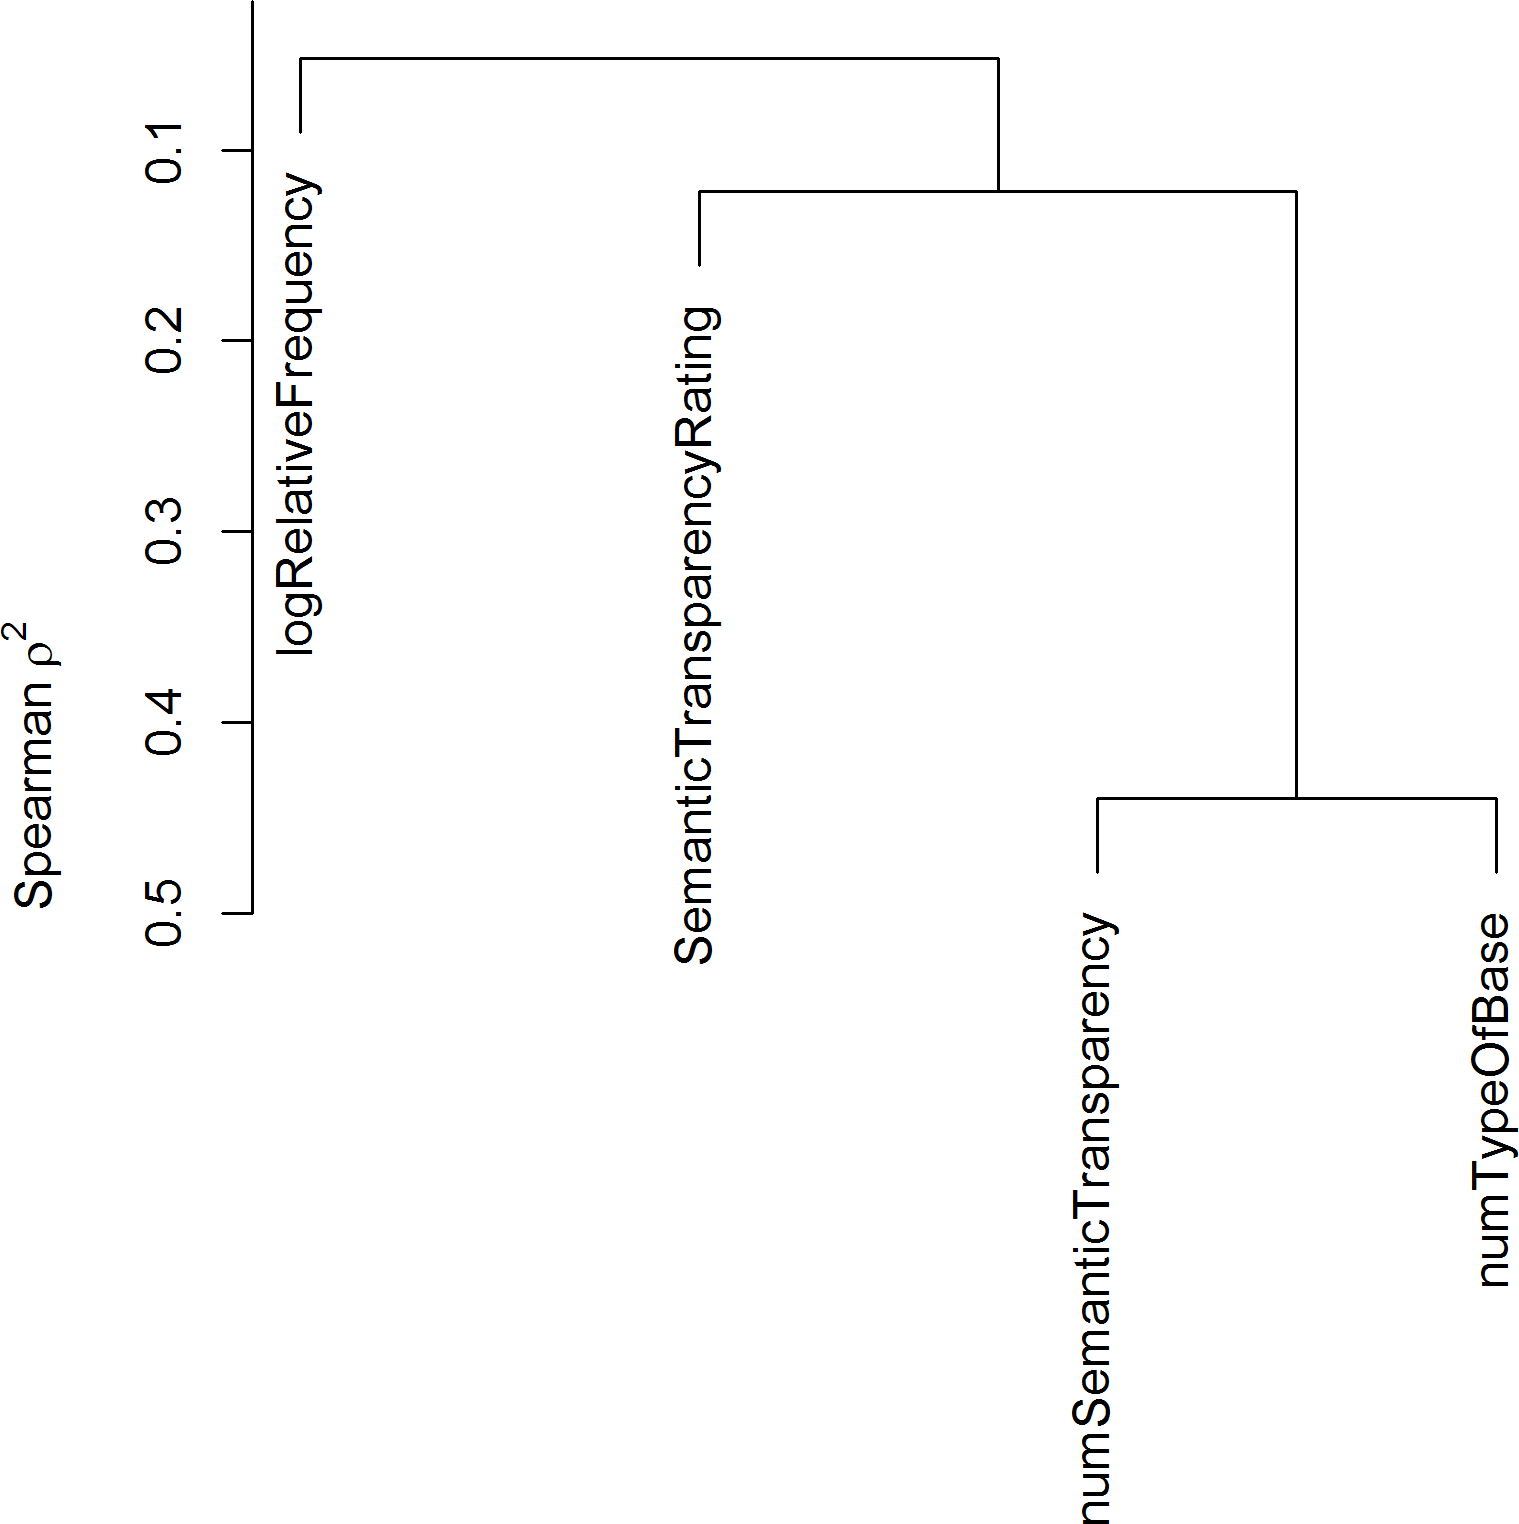
\includegraphics[scale=0.5]{images/Experiment/clusterAnalysisDecomposabilityExperimentAllTokens.png}
 	\caption{Dendrogram of the four decomposability measures for all words in the experimental study}
 	\label{fig:cluster experiment all affixes}
 \end{figure*}
 
\figref{fig:cluster experiment all affixes} displays the relation between the variables in a dendrogram. On the y-axis the squared Spearman correlation score between the variables is displayed. 
The figure shows two splits which structure the variables into three clusters. The lower the split in the figure is, the higher is the correlation between the variables of the pertinent cluster.
The first split is positioned in the upper part of the figure and separates the  variable log\textsc{RelativeFrequency} from all other variables. That log\textsc{RelativeFrequency} forms its own cluster in the upper part of the figure indicates the dissimilarity of this variable to the other \is{decomposability measure}decomposability variables. 
The second split, which is also positioned in the upper part of the figure, separates the variable \textsc{SemanticTransparencyRating} from \textsc{numSemanticTransparency} and \textsc{numTypeOfBase}. This indicates that \textsc{SemanticTransparencyRa-ting} is also rather dissimilar from the other \is{decomposability measure}decomposability variables. 
\textsc{numSemanticTransparency} and \textsc{numTypeOfBase} are much more similar to each other. This is indicated by the cluster they form in the lower part of the figure. 

  \begin{figure*}
  	
  	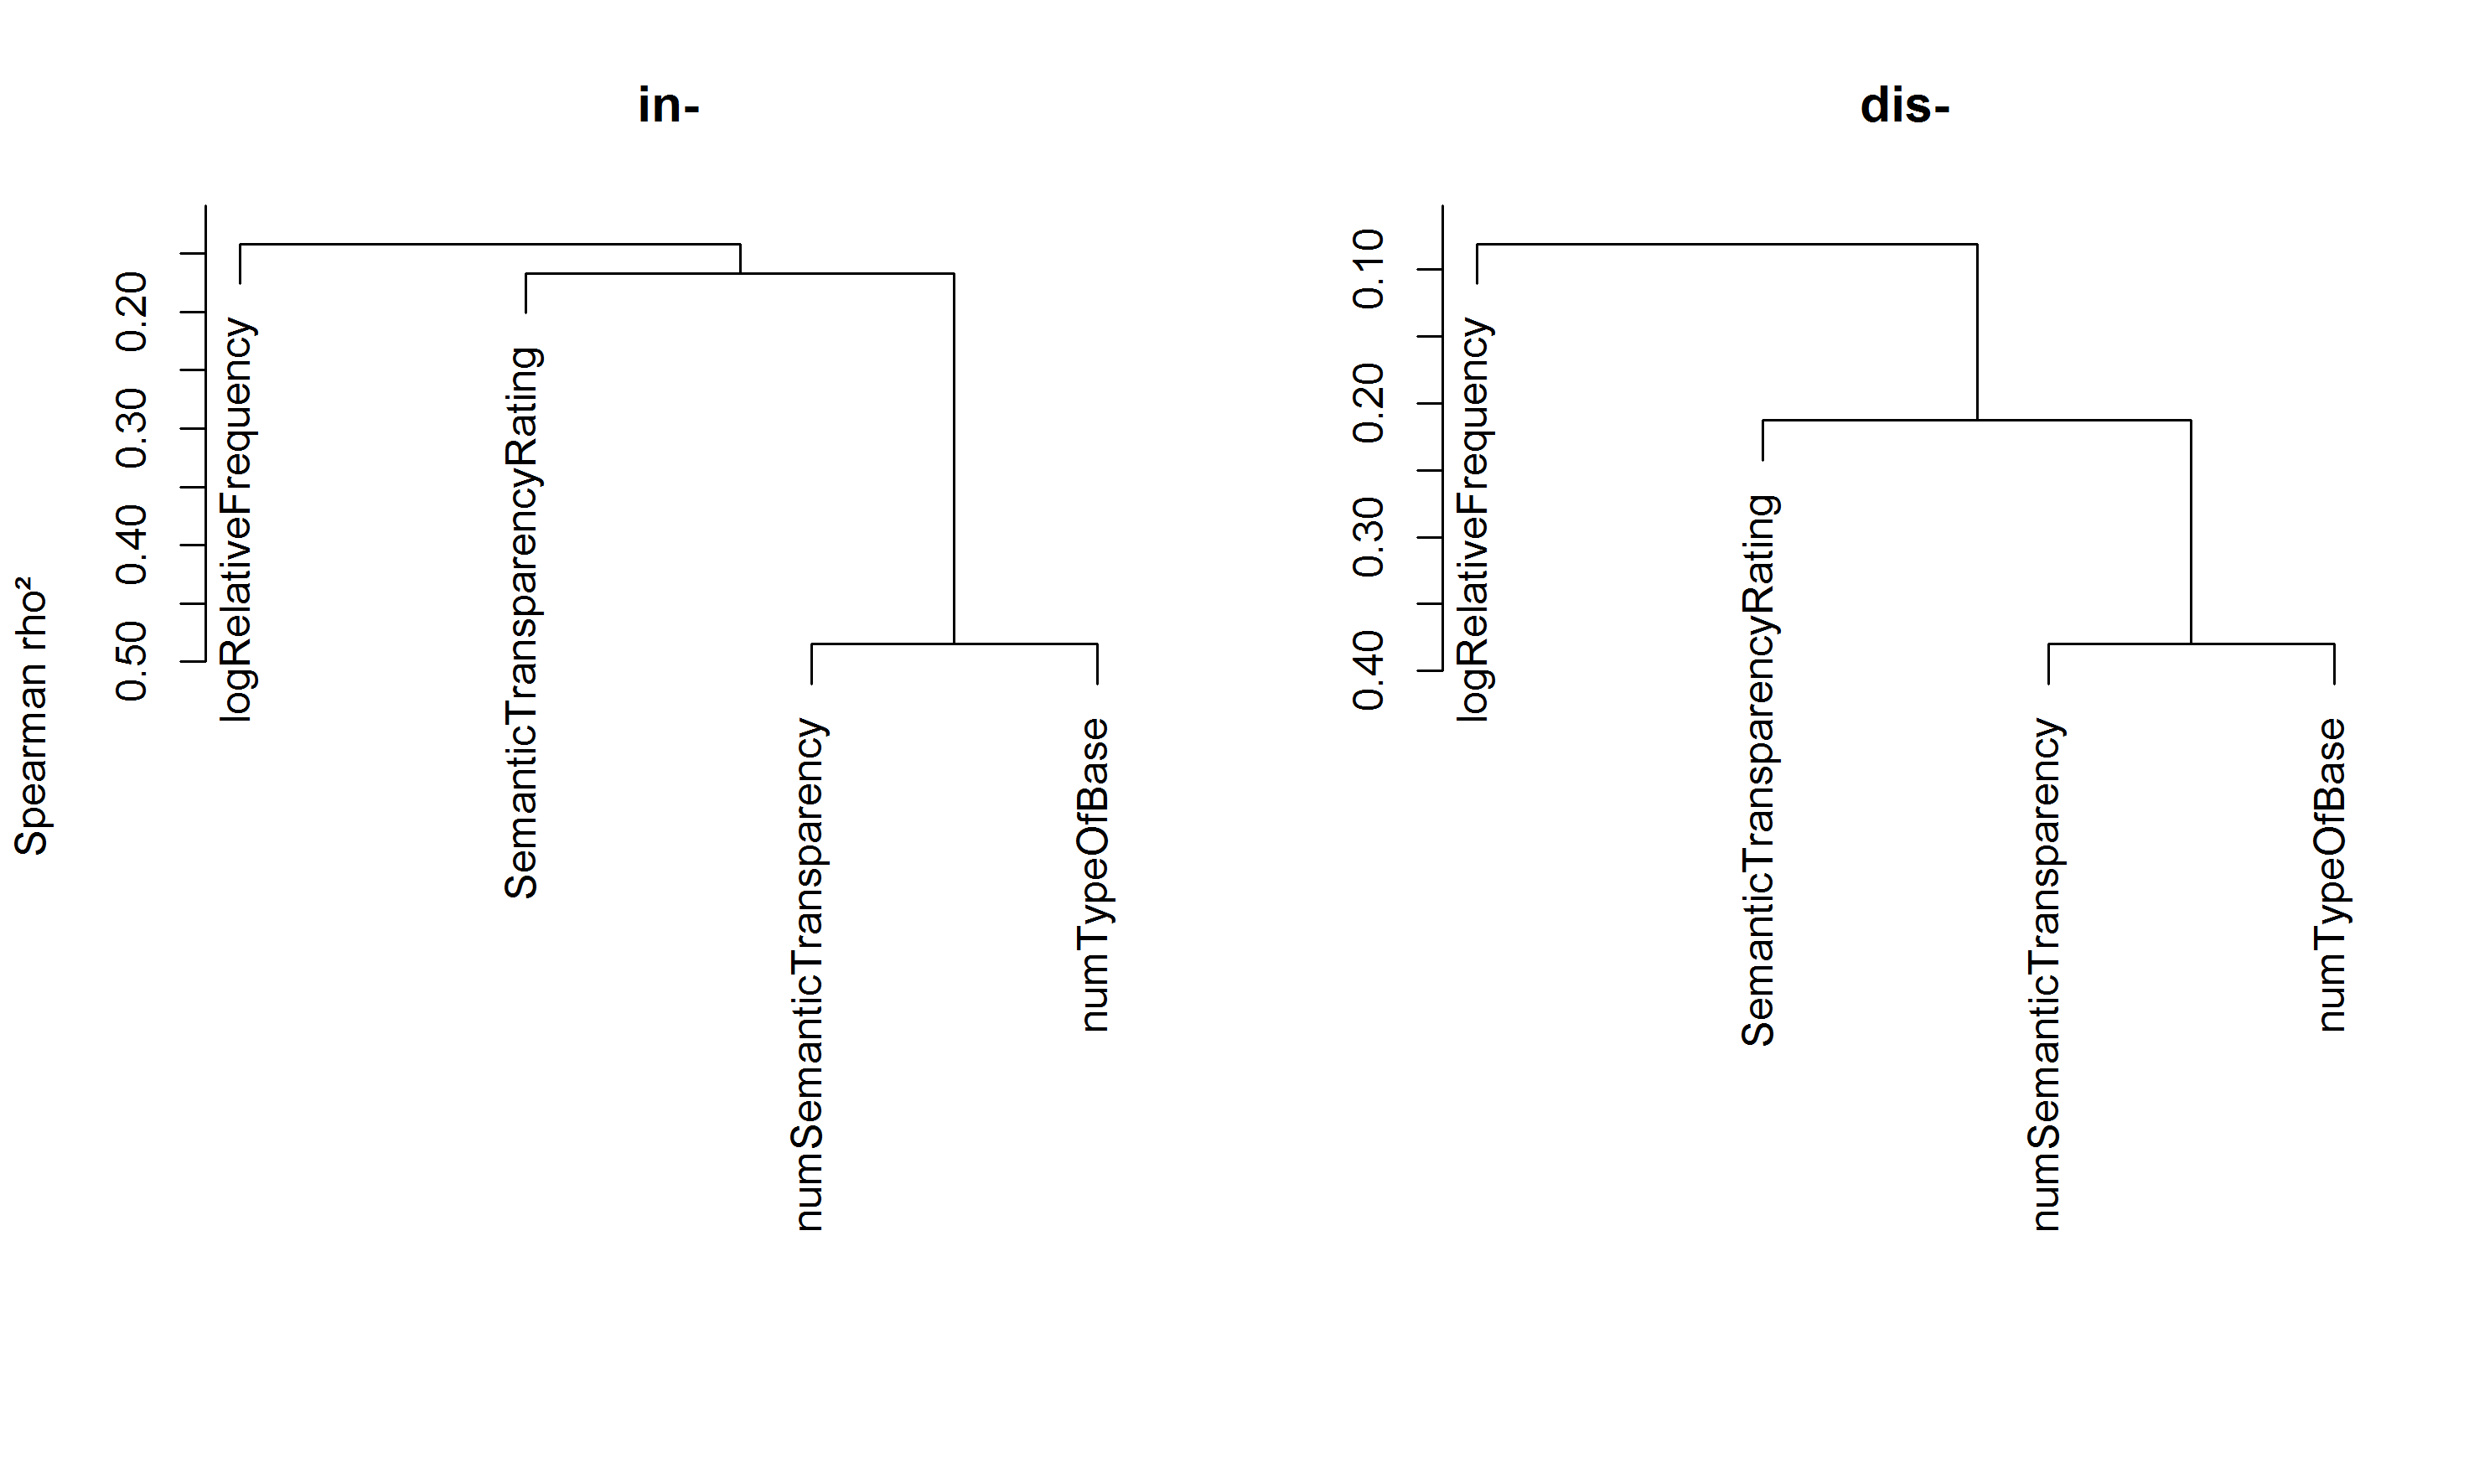
\includegraphics[scale=0.5]{images/Experiment/clusterAnalysisDecomposabilityExpDisAndIn.png}
  %	\vspace*{-20mm} 
  	\caption{Dendrogram of the four decomposability measures for \prefix{in} and \prefix{dis}prefixed words in the experimental study}
  	\label{fig:cluster experiment dis and in}
  	%	\vspace*{-10mm} 
  \end{figure*}
  
 The results of the \is{hierarchical cluster analysis}{cluster analyses} for \is{in-}\prefix{in} and \is{dis-}\prefix{dis} are displayed in the dendrograms in \figref{fig:cluster experiment dis and in}. The results resemble the result of the first \is{hierarchical cluster analysis}{cluster analysis}.
 For both prefixes, the variables \textsc{numSemanticTransparency} and \textsc{numTypeOfBase} cluster together in the lower part of the figure. This means that the correlations between these two variables are rather high. Log\textsc{RelativeFrequency} and \textsc{SemanticTransparencyRating} do not correlate to a high degree with any other variable.
 For \is{dis-}\prefix{dis}, \textsc{SemanticTransparencyRating} is a little more similar to \textsc{numSemanticTransparency} and \textsc{numTypeOfBase} than for \is{in-}\prefix{in}. 
 Overall, log\textsc{RelativeFrequency} and \textsc{SemanticTransparencyRating} are, however, not very similar to the other \is{decomposability measure}decomposability variables in both data sets. 

 
 To sum up, the \is{hierarchical cluster analysis}{cluster analyses} have revealed that the two variables \textsc{Semantic-Transparency} and \textsc{TypeOfBase} are very similar. The two variables log\textsc{Rela\-tiveFrequency} and \textsc{SemanticTransparancyRating}, in contrast, barely correlate with any other \isi{decomposability} variable.
This outcome only partly resembles the outcome of the corpus study. While both studies found that \textsc{SemanticTransparency} and \textsc{TypeOfBase} are very similar, and that the variable log\textsc{RelativeFre-quency} is different, the outcome for \textsc{SemanticTransparencyRating} differs between the studies. 
In the corpus study, \textsc{SemanticTransparencyRating} is very similar to \textsc{SemanticTransparency} and to \textsc{TypeOfBase}. In the experimental stu-dy, the correlations between \textsc{SemanticTransparencyRating} and \textsc{TypeOfBase}, and between \textsc{SemanticTransparencyRating}  and \textsc{SemanticTransparency} are not very high. They are barely higher than the ones between log\textsc{RelativeFre-quency} and the three other \is{decomposability measure}decomposability variables. 
This means that while ratings of the corpus study were highly influenced by the \isi{semantic transparency} and the type of base of a derivative, the ratings of the experimental study were less influenced by these factors.

 
 %Possible reasons for differences in ratings
 One possible explanation for this difference between the corpus and the experimental ratings is that the two groups of raters might have differed with regard to their definition of \isi{decomposability}, and that this difference might have led to different rating strategies. This explanation especially makes sense regarding the fact that the experimental raters were younger and mostly students, while the corpus raters represent a random selection of people of different ages. It might be the case that the younger raters, who are still in school, used a rule-based rating strategy which is based on their knowledge about word-formation, while the older raters, who might not have such knowledge, relied on information about \isi{semantic transparency} and the type of base of a word. 

 The relation between the \is{decomposability measure}decomposability measures has important implications for the interpretation of possible \isi{decomposability} effects on duration. As in the corpus study, possible effects of the \is{decomposability measure}decomposability variables \textsc{Semantic-Transparency} and \textsc{TypeOfBase} can be assumed to be caused by the same underlying property. 
 Effects of log\textsc{RelativeFrequency} and \textsc{SemanticTransparencyRating} on duration are probably caused by different underlying properties (see also \sectref{The Relation between Decomposability Measures} for a discussion of the concept \isi{decomposability} and its operationalization in the study).
 
\begin{table}
	\begin{tabularx}{\textwidth}{p{2.25cm}lQ}
	\lsptoprule
	& Segmentability hierarchy &	Additional assumption\\
		\midrule
	Semantic\newline Hierarchy & \prefix{un} > \{\prefix{dis}, \prefix{in}\textsubscript{\textsc{Neg}}\}>  \prefix{in}\textsubscript{\textsc{Loc}} > \suffix{ly}& lexical meaning over productivity, transparency and type of base \\\tablevspace
	Non-Semantic Hierarchy	&  	\prefix{un} > \suffix{ly} > \{\prefix{dis}, \prefix{in}\textsubscript{\textsc{Neg}}\}>  \prefix{in}\textsubscript{\textsc{Loc}}& productivity, transparency and  type of base	over lexical meaning \\
	\lspbottomrule
\end{tabularx}
	\caption{Lexical segmentability hierarchies of  affixes\label{fig:Segmentability hierarchies of  affixes repetition 3}\is{productivity}}
\end{table}


\subsection{The segmentability of the affixes: A comparison}\label{Exp The Segmentability of the Affixes: A Comparison}\largerpage[-1]
\tabref{fig:Segmentability hierarchies of  affixes repetition 3} displays the \isi{segmentability} hierarchies proposed in \sectref{comparison affixes}. To see whether the hierarchies are borne out by the data, it is necessary to compare the \isi{segmentability} of the five investigated affixes as found in the data. If the hierarchies are valid, the \isi{segmentability} of the affixes should pattern according to the hierarchies. 
As explained above, in the experimental study, only the distribution of the variable \textsc{SemanticTransparencyRating} across affixes was compared to investigate the \isi{segmentability} of the affixes.


\tabref{tbl:Exp distribution semantic transparency rating} shows the distribution of \textsc{SemanticTransparencyRating} for each affix. Next to the total number of tokens, the percentage of tokens with the pertinent rating per affix is given. 


\begin{table}
	\caption{Semantic Transparency Rating  by affix\label{tbl:Exp distribution semantic transparency rating}}
    \resizebox{\textwidth}{!}{%		
		\begin{tabular} {lr@{ }rr@{ }rr@{ }rr@{ }rr@{ }r}
            \lsptoprule
			\textsc{SemanticTrans-}& & & &&   \\
			\textsc{parencyRating }&\multicolumn{2}{c}{\prefix{in}\textsubscript{\textsc{Loc}}  }&\multicolumn{2}{c} {\suffix{ly}} & \multicolumn{2}{c} {\textit{dis-}} & \multicolumn{2}{c} {\prefix{in}\textsubscript{\textsc{Neg}} }   & \multicolumn{2}{c} {\prefix{un} }   \\
			\midrule
			
			1 - most decomposable             &  201 &(35\%) &   747& (62\%)  &   590& (71\%)    & 1225 &(71\%)   & 1868& (92\%)        \\
			2                                 &  81  &(14\%) &   213&(18\%)   & 119&(14\%) &  244&(14\%)&   129&(6\%)  \\
			3								  &  100 &(17\%) &   182&(15\%)   &   69&(8\%)&  148&(9\%) & 37&(2\%)    \\
			4 -  least decomposable           &  194 &(34\%) &    63&(5\%)    & 51&(6\%) &  100&(6\%) &  5 &(\textless 1\%)  \\
			\lspbottomrule			
		\end{tabular}}
\end{table}

%Results
Overall most  items were rated as quite easy to decompose, i.e. the majority of items was rated with 1. This distribution supports the suspicion that experimental raters might have used a rule-based approach in their rating, i.e. they categorically rated items as either decomposable or not decomposable. 
However, the table also shows that there is variation in the ratings. 
Crucially, there are differences in the distribution of ratings between affixes. Kruskal-Wallis tests ($p<0.05$) revealed that all differences between affixes, except the one between \is{negative in-}negative \prefix{in} and \is{dis-}\prefix{dis}, are significant.



The prefix \is{un-}\prefix{un} is rated as the most segmentable affix. 
 Locative \prefix{in} is rated as the least segmentable affix, and the other three affixes pattern in between. 
  This pattern partly resembles the pattern found in the corpus study. In both studies, \is{un-}\prefix{un} was rated the most segmentable affix, and \is{locative in-}locative \prefix{in} was rated the least segmentable affix. 
 However, differently from the corpus study, in the experimental study, the suffix \is{-ly}\suffix{ly} is rated as slightly less decomposable than \is{negative in-}negative \prefix{in} and \is{dis-}\prefix{dis}. In the corpus study, \is{-ly}\suffix{ly} was rated as the second most segmentable affix after \is{un-}\prefix{un}.


The difference in the rating of the suffix \is{-ly}\suffix{ly} between corpus and experimental rating is very interesting with regard to the \isi{segmentability} status of the suffix and the \isi{segmentability} hierarchies. The placement of \is{-ly}\suffix{ly} in the \isi{segmentability} hierarchies highly depends on the definition of \isi{decomposability}. On the one hand, \is{-ly}\suffix{ly} is very segmentable in terms of its \isi{productivity}, its transparency and the types of bases it takes, on the other, the suffix does not feature a clear lexical meaning and its status as a derivational suffix is contested in the literature (see, for example, \citealt{Zwicky.1995,Plag.2003,Giegerich.2012,Bauer.2013} for discussion). Depending on one's definition of \isi{decomposability}, \is{-ly}\suffix{ly} is either a very segmentable affix (Non-Semantic Segmentability Hierarchy) or an affix with very low \isi{segmentability} (Semantic Segmentability Hierarchy) (see also discussion in \sectref{ly}). 

The different \isi{segmentability} patterns found in the corpus and the experimental study mirror the ambiguous \isi{segmentability} status of \is{-ly}\suffix{ly}. In turn, they can be interpreted to provide support for the validity of both \isi{segmentability} hierarchies. 
In the corpus study, the suffix \is{-ly}\suffix{ly} is the second most segmentable affix. This is in line with the Non-Semantic Segmentability Hierarchy. 
In the experimental study, the suffix \is{-ly}\suffix{ly} is rated as one of the least segmentable affixes. This is in line with the Semantic Segmentability Hierarchy.\footnote{Note, however, that according to the Semantic Segmentability Hierarchy, \is{locative in-}locative \prefix{in} is expected to be less segmentable than \is{-ly}\suffix{ly}. This is not the case. }
The \isi{segmentability} pattern of the prefixes provides further support for the validity of the two hierarchies. In both studies, the \isi{segmentability} of the prefixes patterns according to both hierarchies. 



\subsection{Summary}\largerpage

% Summary
The investigation of the relation of the \is{decomposability measure}decomposability measures has revealed that while the two variables \textsc{SemanticTransparency} and \textsc{TypeOfBase} are very similar to each other, the two variables log\textsc{RelativeFrequency} and \textsc{Semantic-TransparencyRating} are different from all other \is{decomposability measure}decomposability measures.
This has important implications for the interpretation of possible \isi{decomposability} effects on duration. While possible effects of \textsc{SemanticTransparency} and \textsc{TypeOfBase} can be assumed to be caused by the same underlying property, possible effects of log\textsc{RelativeFrequency} and \textsc{SemanticTransparencyRating} on duration are probably caused by different underlying properties.



With regard to the \isi{segmentability} of the affixes, the experimental rating shows a similar pattern as the corpus study. As in the corpus study, the prefix \is{un-}\prefix{un} is rated as the most segmentable affix, and \is{locative in-}locative \prefix{in} is rated as the least segmentable affix. However, the suffix \is{-ly}\suffix{ly} is rated differently in the experimental rating, i.e. it is the second least segmentable affix, whereas it is rated the second most segmentable affix in the corpus. The different ratings for \is{-ly}\suffix{ly} in the corpus and the experimental study mirror the ambiguous \isi{segmentability} status of the affix and its different placements in the \isi{segmentability} hierarchies. 



\section{Duration}


\subsection{Analyses} \label{analsyses duration experiment}

As in the corpus study, each affix (and each allomorph, if there was more than one) was investigated separately, i.e. five subsets were created, one for the \is{un-}\prefix{un} words, one for the /ɪn/-words, one for the \is{im-}/ɪm/ -words, one for the \is{dis-}\prefix{dis}words, and one for the \is{-ly}\suffix{ly}-words.

To get a first impression of the \isi{gemination} pattern, and to test whether \isi{gemination} is a categorical or a gradient phenomenon, the first durational analysis consisted of investigating the raw distribution of consonant duration in each subset (cf. \textit{Nature of {gemination}: Predictions }in \sectref{predictions nature of gemination}). To see whether the distributions differ between environments, I generated boxplots for each environment of each subset. 
If the boxplots indicate a bimodal distribution with doubles having a higher mean than singletons, one can assume \isi{gemination} to be categorical (see \sectref{analyses dur corpus} for detailed description of the analyzing strategy). 

After investigating the raw distributions across environments, I fitted two linear mixed effects \is{regression model}{regression models} to each subset. 
The first model predicts \is{absolute duration}absolute consonant duration with all complex words of a given subset (\textit{complex model}). These models are very similar to the models fitted in the corpus study, i.e. they include complex words with a phonological double (e.g. \textit{unnatural}) and complex words with a phonological singleton (e.g. \textit{uneasy}). 
The second model, the \textit{complete model,} predicts \is{absolute duration}absolute consonant duration with all tokens of a pertinent subset, i.e. the models also include base words with a singleton (e.g. \textit{natural} or \textit{real}), and simplex words with an orthographic double (e.g. \textit{dissertation} or \textit{belly}). The complete models were fitted to test whether phonological doubles are longer than corresponding singletons in base words, and whether \isi{gemination} is affected by the presence of orthographic doubles. 

In addition to the two models for each subset, one model which directly compares \is{un-}\prefix{un} and /ɪn/-prefixed words was fitted. This model was fitted to test whether the three prefixes \is{un-}\prefix{un}, \is{locative in-}locative \prefix{in} and \is{negative in-}negative \prefix{in} deviate in their durational patterns. No other affixes were directly compared in one model as inherent durational differences between different types of consonants are too severe to be investigated in one model. Note that in the model featuring \is{un-}\prefix{un} and /ɪn/-prefixed words, some variables cannot be investigated because there are systematic differences in the distribution of variables between the prefixes. Details will be given in the pertinent section.


The dependent variable of all models was \is{absolute duration}absolute consonant duration. Based on the findings of the corpus study, no models with \isi{relative duration} as the dependent variable were fitted.  The corpus study revealed that relative consonant duration is a much weaker measure of \isi{morphological gemination} in English than \is{absolute duration}absolute consonant duration (see \sectref{Summary Corpus Study}).

Only the complex models tested the effects of the \is{decomposability measure}decomposability measures on consonant duration, since the \is{decomposability measure}decomposability variables are not applicable to simplex words.
Furthermore, not all \is{decomposability measure}decomposability measures were tested for all affixes. As in the corpus study, only in the complex  \is{in-}\prefix{in} and \is{dis-}\prefix{dis}models all \is{decomposability measure}decomposability variables were included. In the complex \is{-ly}\suffix{ly}-model, only the effects of log\textsc{RelativeFrequency} and \textsc{SemanticTransparencyRating} were tested. In the complex \is{un-}\prefix{un}model, only the effect of log\textsc{RelativeFrequency} was tested. The reason is that the two variables  \textsc{SemanticTransparency} and \textsc{TypeOfBase} do not show enough variation for \is{un-}\prefix{un} and \is{-ly}\suffix{ly}. For \is{un-}\prefix{un}, \textsc{SemanticTransparencyRating} does not show enough variation either.


In the complex models predicting consonant duration with /ɪn/, \is{im-}/ɪm/  and \is{dis-}\prefix{dis}, \isi{collinearity} problems had to be addressed. As discussed in the previous section, the \is{decomposability measure}decomposability variables \textsc{SemanticTransparency} and \textsc{TypeOfBase} highly correlate, and there are also correlations between the other \is{decomposability measure}decomposability variables. It is thus problematic to test all of them simultaneously in the model. Therefore, the effect of these variables was tested by including them individually in the model, and by conducting \is{principal component analysis}principal component analyses (see \sectref{stats} on \is{principal component analysis}principal component analyses). 

In the complete models for the prefixes, the noise variable \textsc{PrecedingSegmentDuration} was not included because the base-initial consonant does not feature a preceding segment. In all models, the two variables \textsc{Speaker} and \textsc{Type} were included as random effects.


As in the corpus study, two types of interactions were tested in each model. First, I tested for interactions which are predicted to affect \isi{gemination} according to the theoretical approaches discussed in Chapter \ref{Theory}. Then, I tested for interactions which, based on previous empirical work and theoretical considerations, can be assumed to affect affixational consonant duration  (see \sectref{analyses dur corpus} for a more detailed description of the two types of interactions). 
 All interactions tested in the experimental study are listed in \hyperref[Appendix G Summaries of tested interactions in experimental study]{Appendix G}.

All models were fitted according to the modeling strategy described in \sectref{stats}.  
The models were generated using the \texttt{lme4} package (\citealt{Bates.2014}), and the plots of the \is{regression model}{regression models} were generated with the \texttt{visreg} package (\citealt{Breheny.2015}). 

After fitting the complex models for each subset, I computed each variable's contribution to the goodness of fit for the final model by checking how the absence of each significant term affects the AIC of the model. The higher the increase of the AIC without a specific term, the more variance is explained by the pertinent term in the model, and the higher is its contribution to the goodness of fit.

\subsection{Overview}
\figref{fig:Expeirment raw duration distribution} depicts the distribution of consonant duration for each environment in each subset using boxplots. In the upper row, the distribution for \is{un-}\prefix{un} is shown in the left panel, the one for /in/
%\todo{do you mean /in/ or /ɪn/?} 
is shown in the middle panel, and the one for \is{im-}/ɪm/  is shown in the right panel. The distribution for \is{dis-}\prefix{dis} is shown in the lower left panel, and the one for \is{-ly}\suffix{ly} in the lower right panel.
The y-axis of each plot displays the duration of the consonant in milliseconds. 

The boxes in each plot represent the distribution of consonant duration for the different environments in each data set. The dot in the middle represents the median duration, and the box itself represents the interquartile range of consonant duration. 
In each plot, the left box(es) represent the environment(s) with a phonological double. They are followed by the box(es) for  complex words with singleton environments and the box(es) for base words with a singleton. For \is{dis-}\prefix{dis} and \is{-ly}\suffix{ly}, the last box (from the left) represents the consonant duration in simplex words with an orthographic double.

\begin{figure*}
	
	\begin{subfigure}
		
		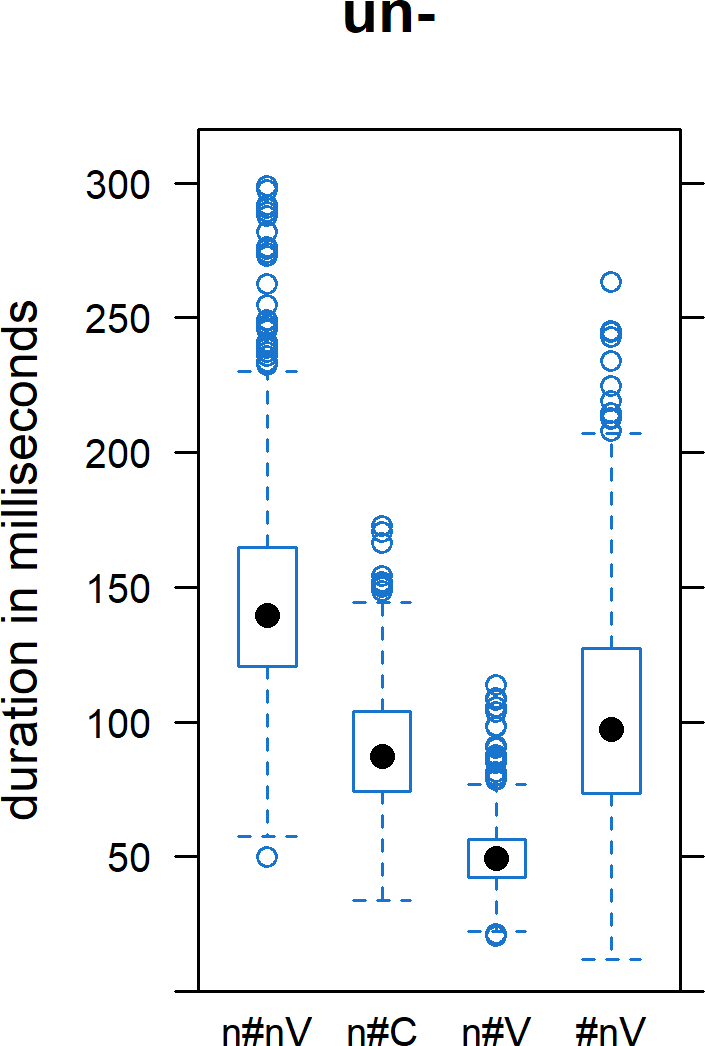
\includegraphics[scale=.55]{images/Experiment/boxUn}
		%	\caption{1a}
		%	\label{fig:sfig1}
	\end{subfigure}%
	~
	\begin{subfigure}
		
		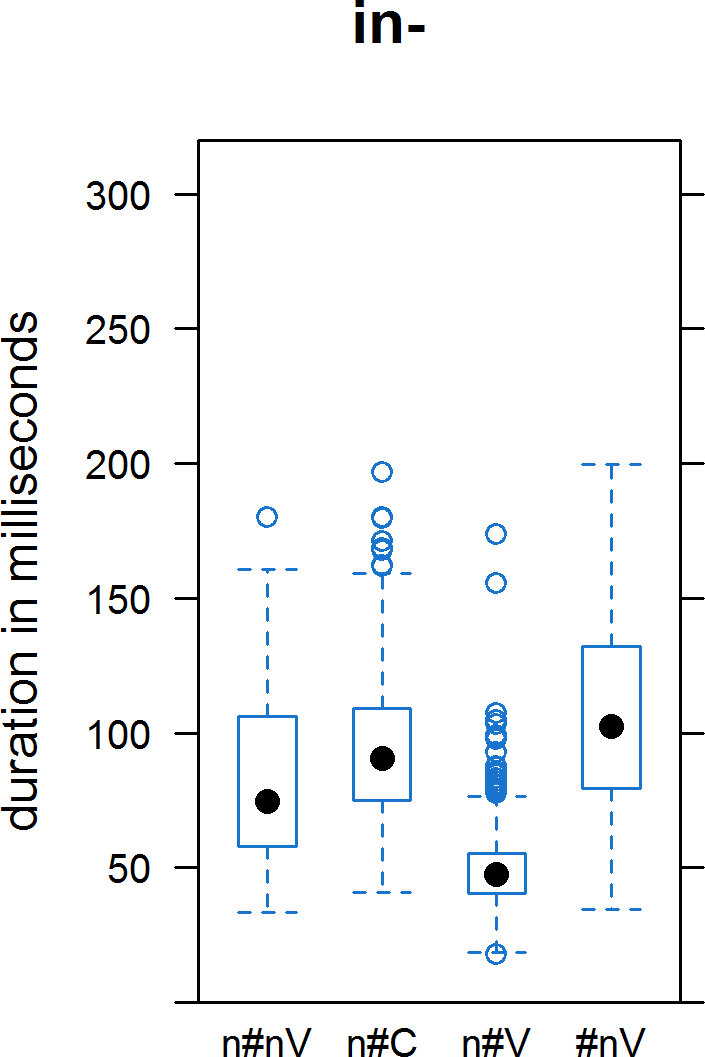
\includegraphics[scale=.55]{images/Experiment/boxIn}
		%	\caption{1b}
		%	\label{fig:sfig2}
	\end{subfigure}
	~
	\begin{subfigure}
		
		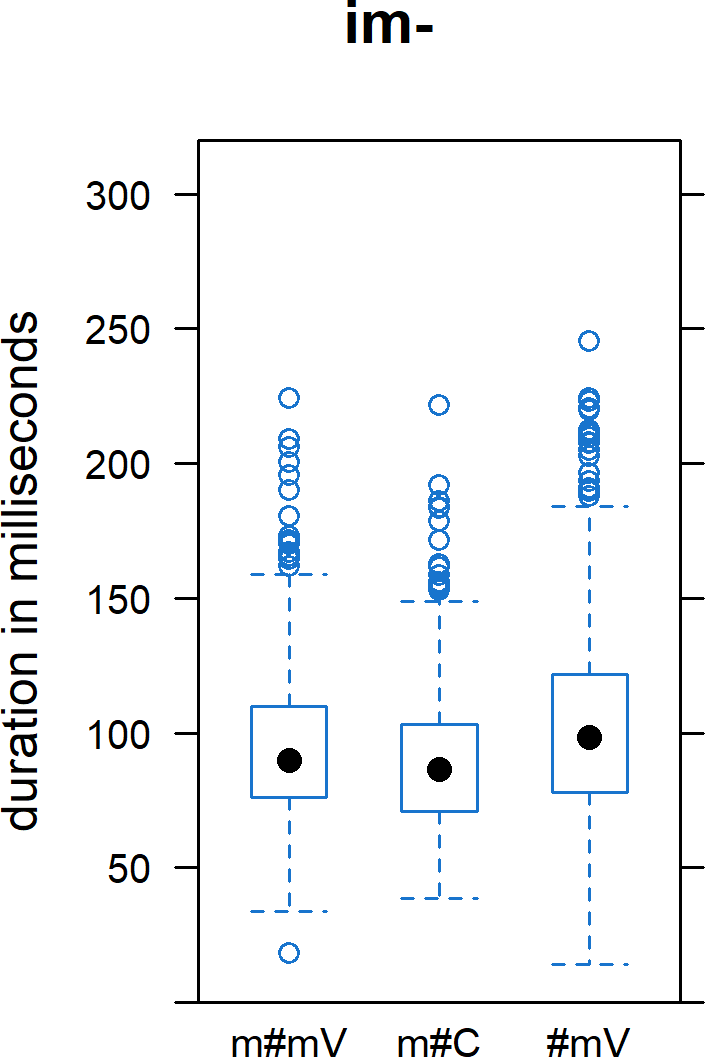
\includegraphics[scale=.55]{images/Experiment/boxIm}
		%	\caption{1b}
		%	\label{fig:sfig2}
	\end{subfigure}
	
	\begin{subfigure}
		
		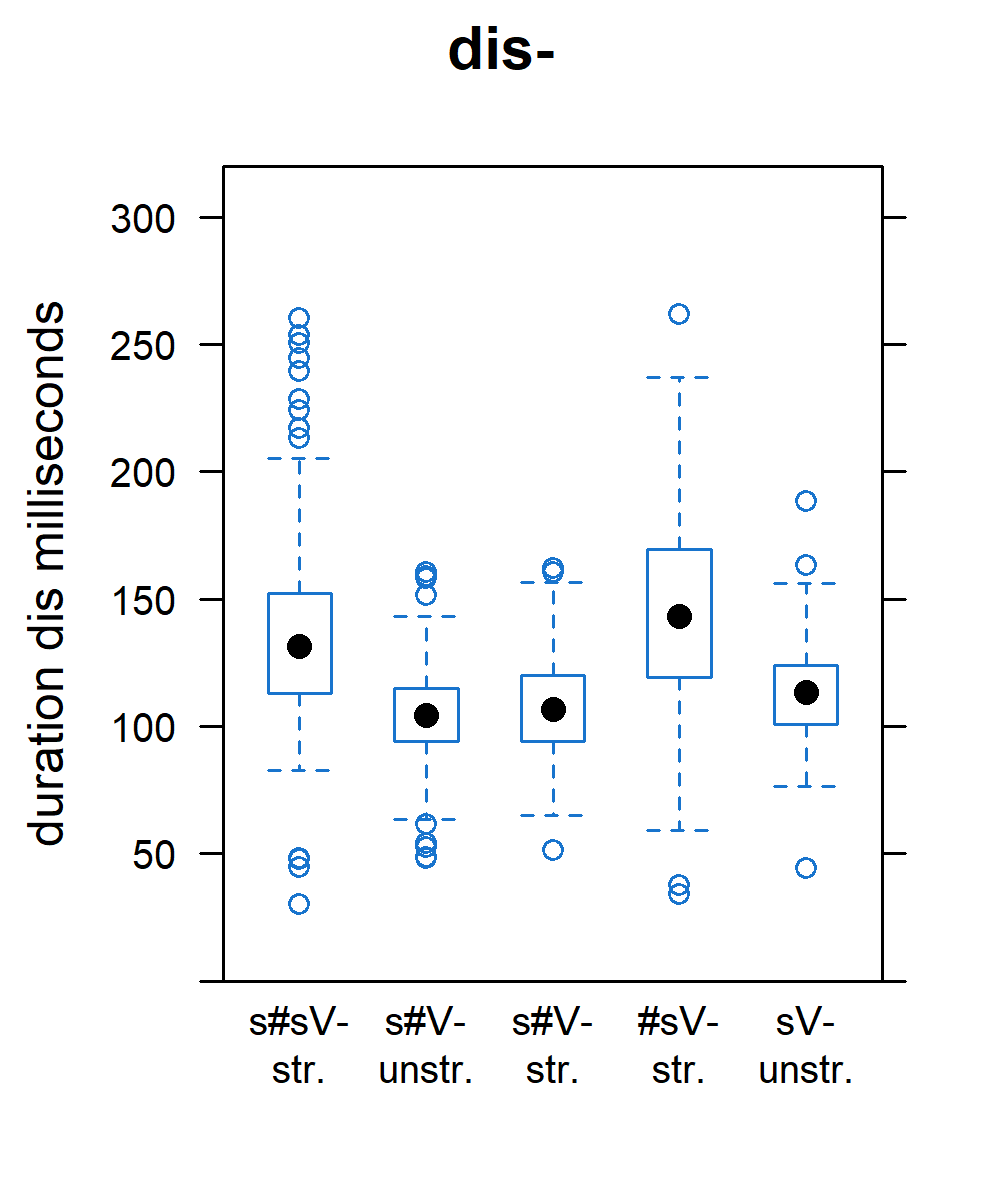
\includegraphics[scale=.55]{images/Experiment/boxDis}
		%	\caption{1b}
		%	\label{fig:sfig2}
	\end{subfigure}
	~
	\begin{subfigure}
		
		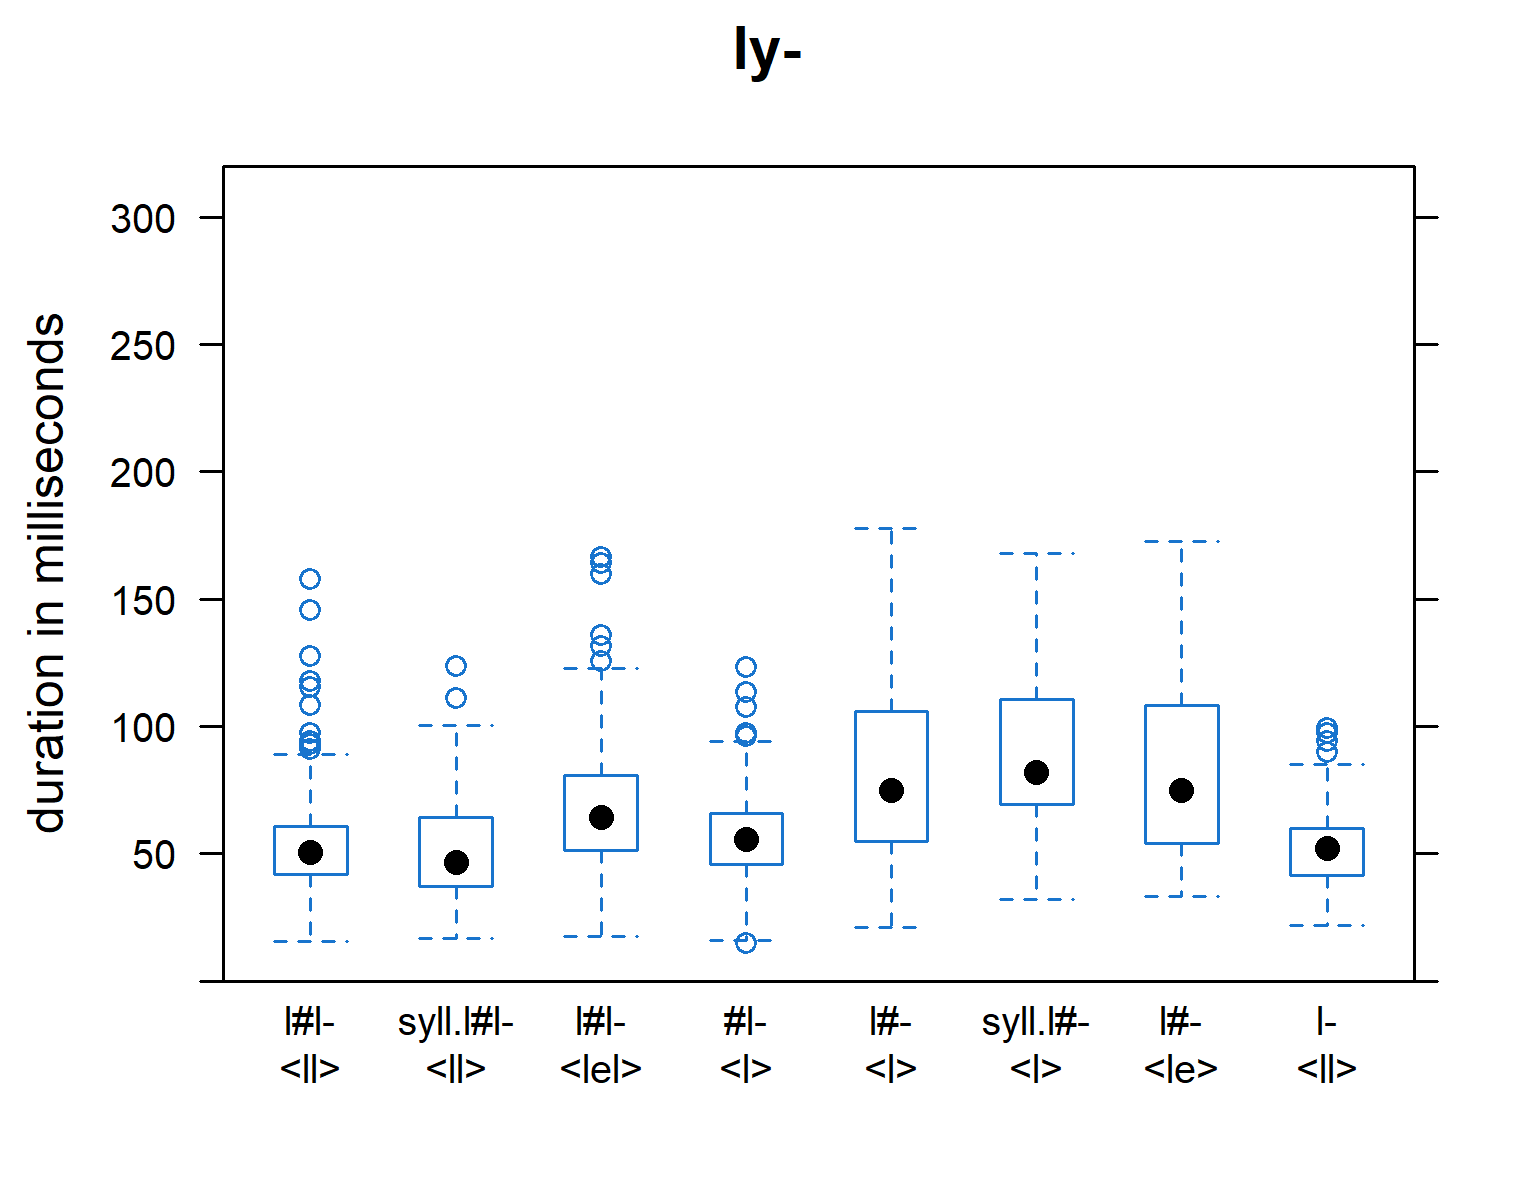
\includegraphics[scale=.55]{images/Experiment/boxLy}
		%	\caption{1b}
		%	\label{fig:sfig2}
	\end{subfigure}				
	
	\caption{Distribution of consonant duration in the five data sets}
	\label{fig:Expeirment raw duration distribution}
\end{figure*}



%un
%plot
For \is{un-}\prefix{un},  the figure shows a clear difference in duration between double and single consonants. Doubles (\texttt{n\#nV}) are longer than singletons in complex words (\texttt{n\#C}, \texttt{n\#V}) and singletons in base words (\texttt{\#nV}). 
  The figure also shows that there is no overlap of the boxes for the doubles and the boxes for the singletons. This indicates a bimodal distribution in the data set with doubles being longer than singletons. 
As the data from the corpus study, the  plot thus suggests that \is{un-}\prefix{un} geminates, and that \isi{gemination} is a categorical phenomenon. 



%in
For /ɪn/, the plot suggests that doubles (\texttt{n\#nV}) are as long as the singletons in complex words followed by a consonant (\texttt{n\#C}) and singletons in base words (\texttt{\#nV}). Only singletons in complex words followed by a vowel (\texttt{n\#V}) are shorter than doubles. 
On the one hand, this durational difference speaks for \isi{gemination} with \is{in-}\prefix{in}, on the other, there is no durational difference between the other singleton levels and the double consonant. This is different from what was found for \is{un-}\prefix{un}.
With regard to the question whether \isi{gemination} is a categorical or a gradient phenomenon, the plot shows that there is no overlap between the box of the doubles (\texttt{n\#nV}) and the box of the singletons with a following vowel (\texttt{n\#V}) for /ɪn/. In other words, the distribution of duration of doubles and singletons with a following vowel seems to be bimodal. This suggests that, if there is \isi{gemination} with /ɪn/, it is probably categorical.

%im
For \is{im-}/ɪm/, no difference in consonant duration can be seen between the three environments (\texttt{m\#mV}, \texttt{m\#C}, \texttt{\#mV}). The plot thus suggests \isi{degemination} with \is{im-}/ɪm/. However, 
it is yet unclear whether the allomorph \is{im-}/ɪm/  really degeminates, or whether \isi{gemination} with \is{im-}/ɪm/  depends on additional factors which are not taken into account when comparing the raw durations of doubles and singletons. 

%dis

For \is{dis-}\prefix{dis}, the plot shows that doubles (\texttt{s\#sV-str.})  are longer than singletons in complex words (\texttt{s\#V-unstr.}, \texttt{s\#V-str.}) and singletons in simplex words with an orthographic double (\texttt{sV-unstr.}). However, singletons in base words (\texttt{\#sV}) are as long as doubles. 
As for /ɪn/, there is thus some evidence for \isi{gemination}, but also some evidence against it.  
The boxes for the double consonants and  for the singleton environments (except for the one for singletons in base words)  hardly overlap. Thus, the distribution of duration of doubles and singletons in complex words seems to be bimodal. This suggests that if there is \isi{gemination} with \is{dis-}\prefix{dis}, it is categorical.


%ly

For \is{-ly}\suffix{ly}, there is a big overlap in the distribution of all environments. Only singletons in base words (\texttt{l\#-<l>}, \texttt{syll.l\#-<l>}, \texttt{l\#-<le>}) seem to have slightly longer durations than singletons in all other environments. Crucially, the plot does not suggest doubles to be longer than singletons of any category. One might thus suspect \isi{degemination} for \is{-ly}\suffix{ly}. 

The overview of the durations of all environments reveals some similarities across all subsets, as well as some differences. 
One similarity is that in all subsets, the consonant in base words is relatively long. This might be due to its word-initial (or word-final) position. 
Furthermore, for the prefixes with a nasal, the nasal is longer before consonants than before vowels. 
Another similarity is that if there are differences between double and singleton consonants, their duration seems to be bimodally distributed. As in the corpus study, the data thus suggest \isi{gemination} to be a categorical phenomenon.

With regard to the question of \isi{gemination}, the affixes seem to behave quite differently. For \is{un-}\prefix{un}, the distributional analysis clearly suggests \isi{gemination}, doubles are longer than all singleton levels. 
For the other affixes, it is less clear whether we find \isi{gemination}. For \is{in-}\prefix{in}, i.e. /ɪn/ and \is{im-}/ɪm/, only one singleton environment features shorter consonants than the double environment.
For \is{dis-}\prefix{dis}, the singleton consonants of all but one environment are shorter than the double consonants. 
For \is{-ly}\suffix{ly}, none of the three double environments is longer than the singleton environments. Further analyses which take more variables into account are needed to clarify the \isi{gemination} pattern of the affixes. 
 In the next subsections I will present such analyses for each subset.


\subsection{The prefix \textit{un-}} \label{un experiment}

\subsubsection{Complex model}


The model predicting consonant duration with all complex \is{un-}\prefix{un}words ($N=2067$) was fitted according to the modeling procedure described in \sectref{stats}. Due to an uneven distribution of the residuals in the initial model, the dependent variable \textsc{AbsoluteConsonantDuration} was Box-Cox-transformed ($\lambda = 0.101$) and 50 outliers were removed (2.4\% of the data).
 After the model was refitted with the transformed dependent variable, it showed a satisfactory distribution of residuals.  The model was then simplified and interactions were tested (see \hyperref[Appendix G Summaries of tested interactions in experimental study]{Appendix G} for a list of all tested interactions).
 
After model simplification five variables remained in the model, \textsc{Environment}, \textsc{Accentuation}, \textsc{LocalSpeechRate}, \textsc{PrePause} and \textsc{PrecedingSegmentDuration}. The two variables \textsc{Environment} and \textsc{Accentuation} interact. The final model is summarized in \tabref{model un complex experiment} which can be found in \hyperref[Appendix H: Model Summaries Experiment]{Appendix H}.


The four noise variables show the expected effects. As in the corpus study, the nasal in \is{un-}\prefix{un} becomes shorter with increasing \isi{speech rate}. 
The nasal in tokens which are preceded by a pause is longer than the nasal in tokens without a preceding pause. This effect of \textsc{PrePause}  can be attributed to \isi{word-initial strengthening}.  
Furthermore, consonant duration depends on the duration of the preceding segment. The longer the preceding segment, the shorter the nasal. 

\begin{figure*}
	
	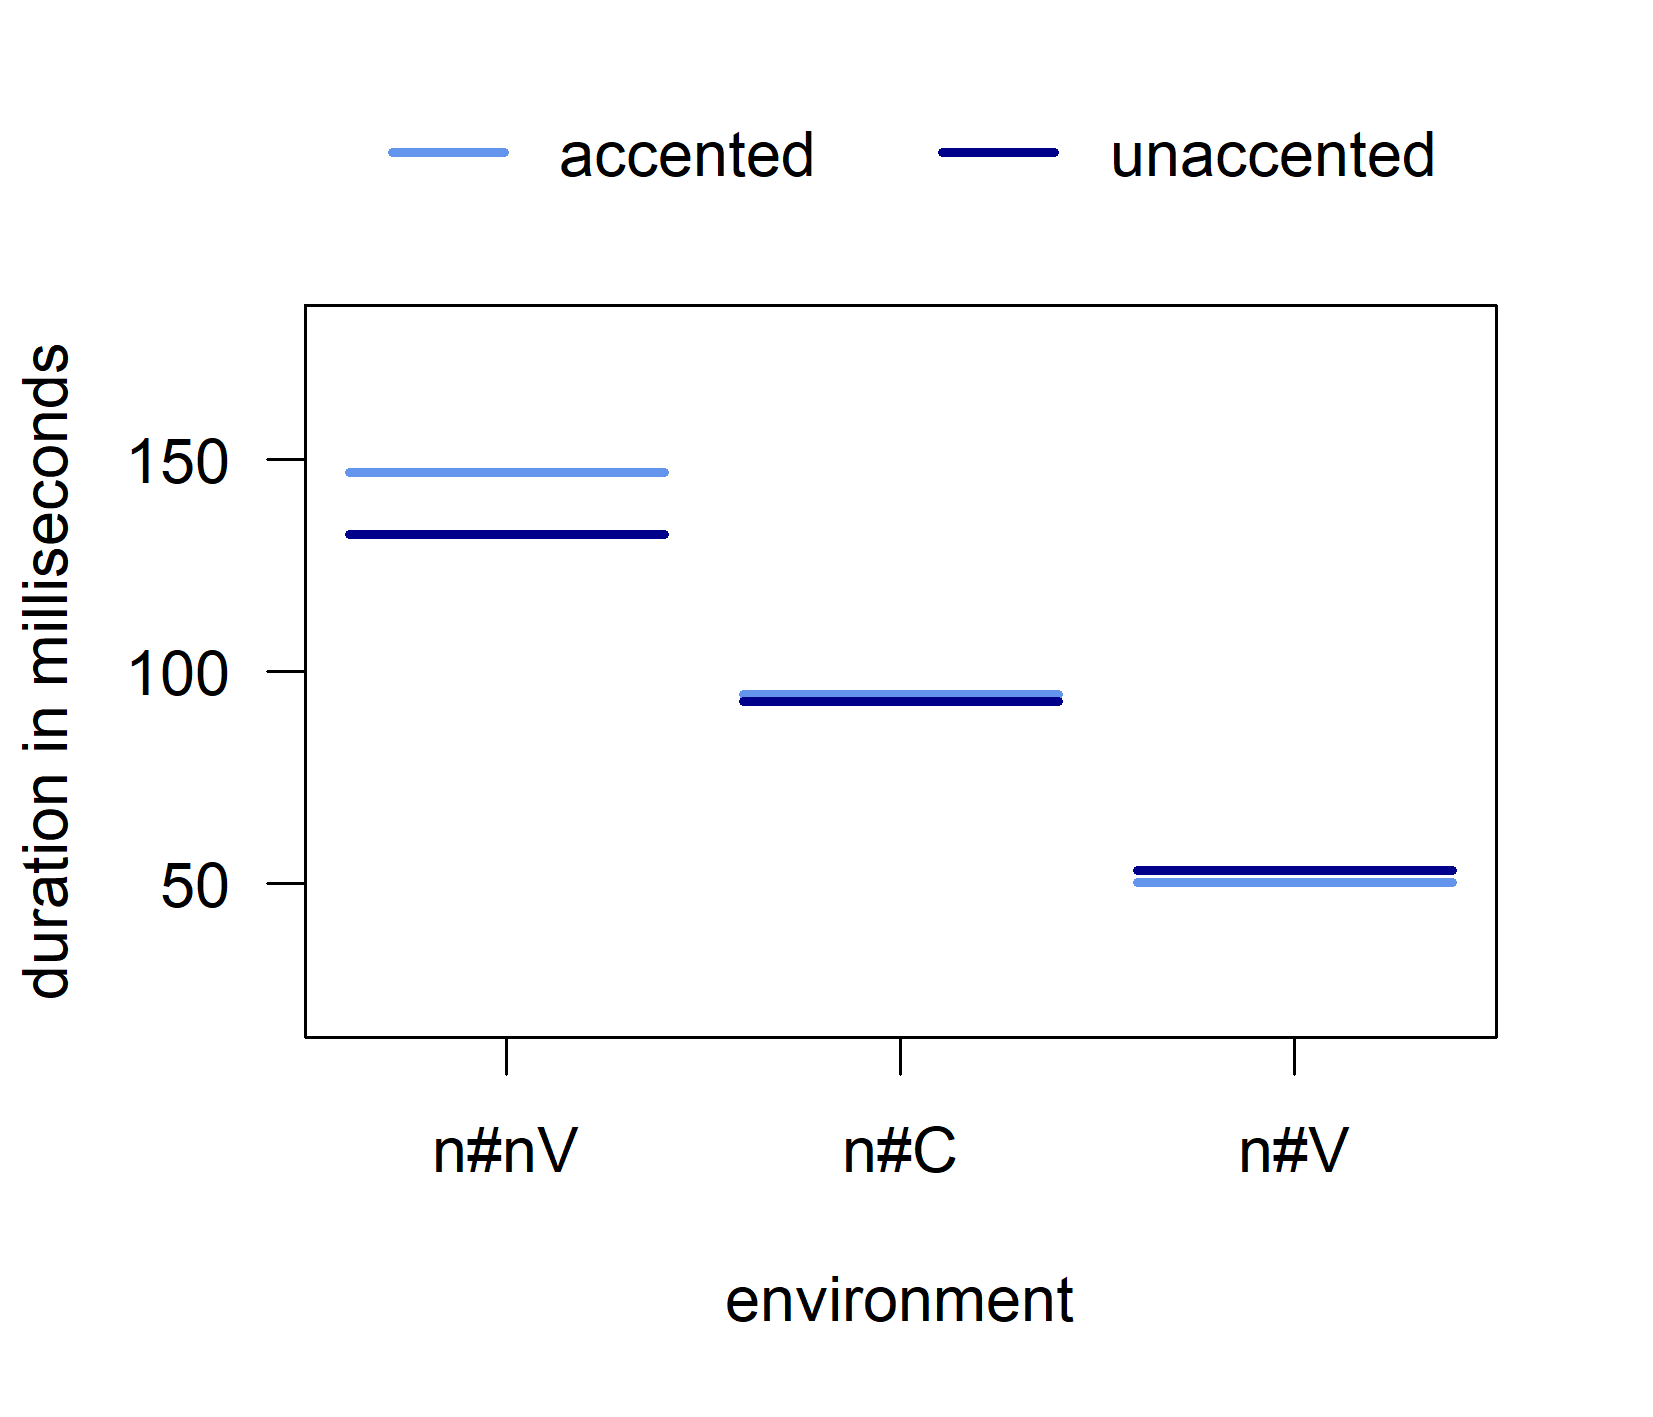
\includegraphics [scale=0.5] {images/Experiment/unModelInterCatAcc}
	\caption{Effect of accentuation by environment on consonant duration in complex \prefix{un}data set}
	\label{fig:NumNasal unComplex experiment}
\end{figure*}


The fourth significant noise variable \textsc{Accentuation} forms an interaction with the variable of interest \textsc{Environment}. The interaction is depicted in \figref{fig:NumNasal unComplex experiment}.
The light blue lines in the figure show the effect of \textsc{Environment} for items in \is{accentuation}accented position, and the dark blue lines show the effect for items in unaccented position. In both conditions, i.e. in the \is{accentuation}accented and in the unaccented condition, there is a significant durational difference between doubles (\texttt{n\#nV}) and singletons (\texttt{n\#C}, \texttt{n\#V}). 
 In \is{accentuation}accented position, doubles are predicted to be 53\,ms longer than singletons followed by a consonant, and 97\,ms longer than singletons followed by a vowel. 
 In unaccented position, doubles are also predicted to be longer than both types of singletons but the durational differences are smaller. The differences are 39\,ms  for singletons followed by a consonant (\texttt{n\#C}), and 80\,ms for singletons followed by a vowel (\texttt{n\#V}). The difference between the two singleton levels is roughly the same in both conditions (45\,ms in \is{accentuation}accented position, 40\,ms in unaccented position).




 The results clearly show that \is{un-}\prefix{un} geminates. Phonological doubles are predicted to be more than twice as long as phonological singletons followed by a vowel, and the predicted singleton-double ratios for consonant adjacent singletons are, depending on \isi{accentuation}, 1:1.4 and 1:1.6. In comparison to former studies, these durational differences are very large (see Sections~\ref{what is gemination} and~\ref{un corpus} for a discussion of durational differences between geminates and their corresponding singletons). 




\begin{figure}
	
	
	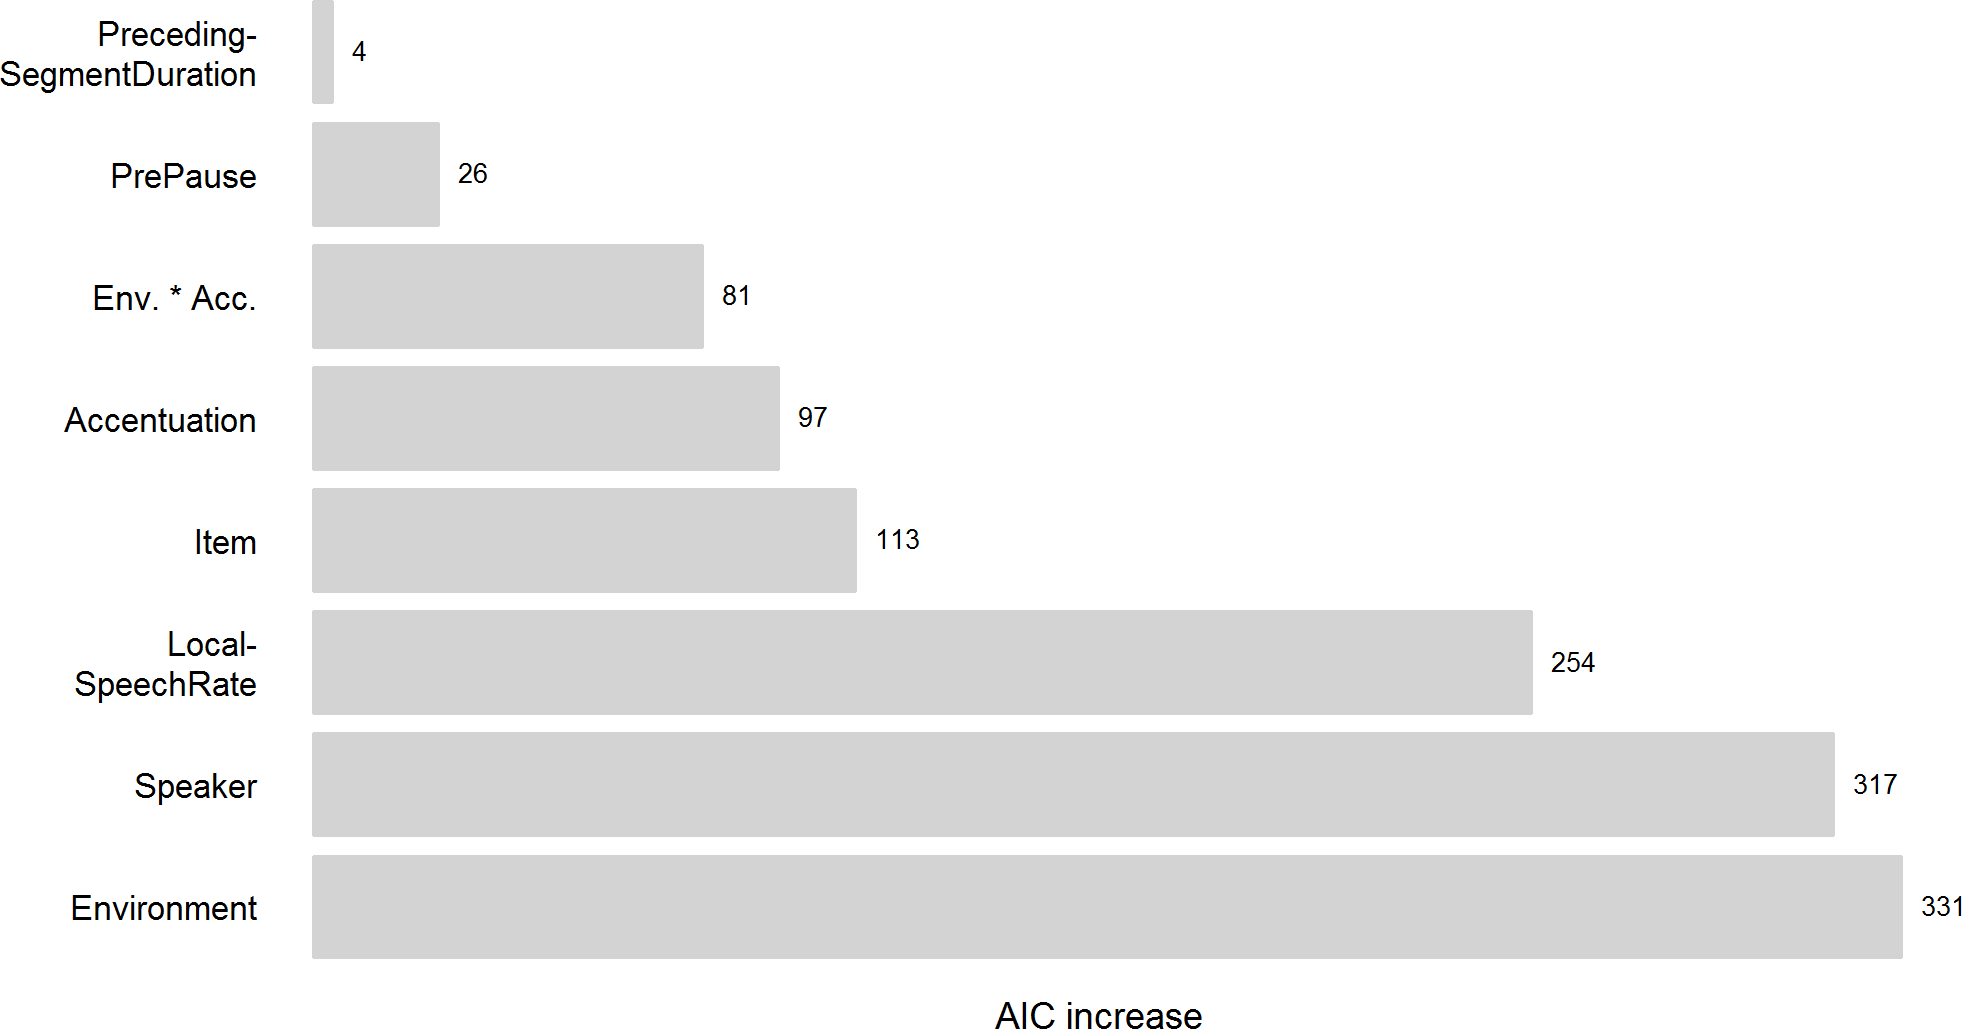
\includegraphics[scale=0.7] {images/Experiment/AICdecreaseUnComplex.png}


	\caption{AIC increase for each variable of the final \prefix{un}model, AIC final model = \textminus11398}
	\label{fig:Effect sozed un Exp unV vs Unn}

\end{figure}



To test the contribution of each variable for the model's goodness of fit, I checked how the absence of each term affects the AIC of the model. \figref{fig:Effect sozed un Exp unV vs Unn} displays the increase of the model's AIC  without each factor. The higher the increase, the more variance is explained by the pertinent factor in the model.\largerpage[-1]



The figure clearly shows that the variable \textsc{Environment} explains most of the variation found in the data. In other words, the absence or presence of a phonological double consonant explains a large portion of the durational differences found in the data.
Furthermore, there are speaker-dependent differences, i.e. different speakers produce the nasal in \is{un-}\prefix{un}prefixed words with different durations. However, it is important to note that while there are overall differences in the duration of the nasal between speakers, all speakers show the same pattern with regard to \isi{gemination}, i.e. all of them produced the double consonants with longer durations than the singletons. 
The third most important variable is \textsc{LocalSpeechRate}. The other noise variables, as well as the interaction, are much less important for the model, i.e. they explain much less of the variance found in the data.


To sum up, the analyses have shown that \is{un-}\prefix{un} clearly geminates, and that the duration of the nasal in \is{un-}\prefix{un}prefixed words is furthermore influenced by phonetic and prosodic factors.
The variables \textsc{Environment} and \textsc{LocalSpeechRate} are two of the most important determiners for consonant duration with \is{un-}\prefix{un}. In addition to \textsc{Speaker}, they explain most of the variance in the data. This result fits in well with the findings of the corpus study, where these two variables were the only two significant predictors for nasal duration with \is{un-}\prefix{un}. 
Furthermore, the two prosodic variables \textsc{Accentuation} and \textsc{PrePause} are rather important predictor variables. The variable \textsc{PrecedingSegmentDuration}, even though significant in the final model, is of less importance. 
%The analyses also indicate that there are item-specific effects which might be related to an item's \isi{stress} pattern and its \isi{frequency}.



\subsubsection{Complete model}\largerpage[-1]

The second \is{un-}\prefix{un}model investigates nasal duration in all tokens of the \is{un-}\prefix{un}data set ($N=2615)$, i.e. it investigates nasal duration in prefixed words and in base words. 
As in the model predicting nasal duration with only complex words, the dependent variable \textsc{AbsoluteConsonantDuration} was Box-Cox-transformed ($\lambda= 0.182$) and outliers ($N=66$, i.e. $ 2.52$\% of the data) were removed to achieve a normal distribution of residuals. The model was then simplified and interactions were tested (see \hyperref[Appendix G Summaries of tested interactions in experimental study]{Appendix G} for a list of all tested interactions). The final model is displayed in \tabref{model un complete experiment} in \hyperref[Appendix H: Model Summaries Experiment]{Appendix H}.


The final model features the variables \textsc{Environment}, \textsc{LocalSpeechRate}, \textsc{BaseInitialStress}, \textsc{Accentuation} and \textsc{PrePause}.
The two noise variables \textsc{Local-SpeechRate} and \textsc{BaseInitialStress} show the expected effects. The faster the \isi{speech rate}, the longer the nasal, and when the base-initial syllable is unstressed the nasal is shorter than when the base-initial syllable is \is{stress}stressed.
The two other noise variables \textsc{Accentuation} and \textsc{PrePause} interact with the variable of interest \textsc{Environment}. Note that there is no three-way interaction between  \textsc{Accentuation}, \textsc{PrePause} and \textsc{Environment}.

\figref{fig:NumNasal Acc un experiment} shows the effect of \textsc{Accentuation} by \textsc{Environment}. The light blue lines represent the estimated durations for words  in \is{accentuation}accented position, the dark blue lines show the estimated durations for words in unaccented position. In both conditions, i.e. in \is{accentuation}accented and unaccented condition, double consonants are predicted to be significantly longer than all types of singletons. This means \is{un-}\prefix{un} geminates, independent of \isi{accentuation}.

\begin{figure*}
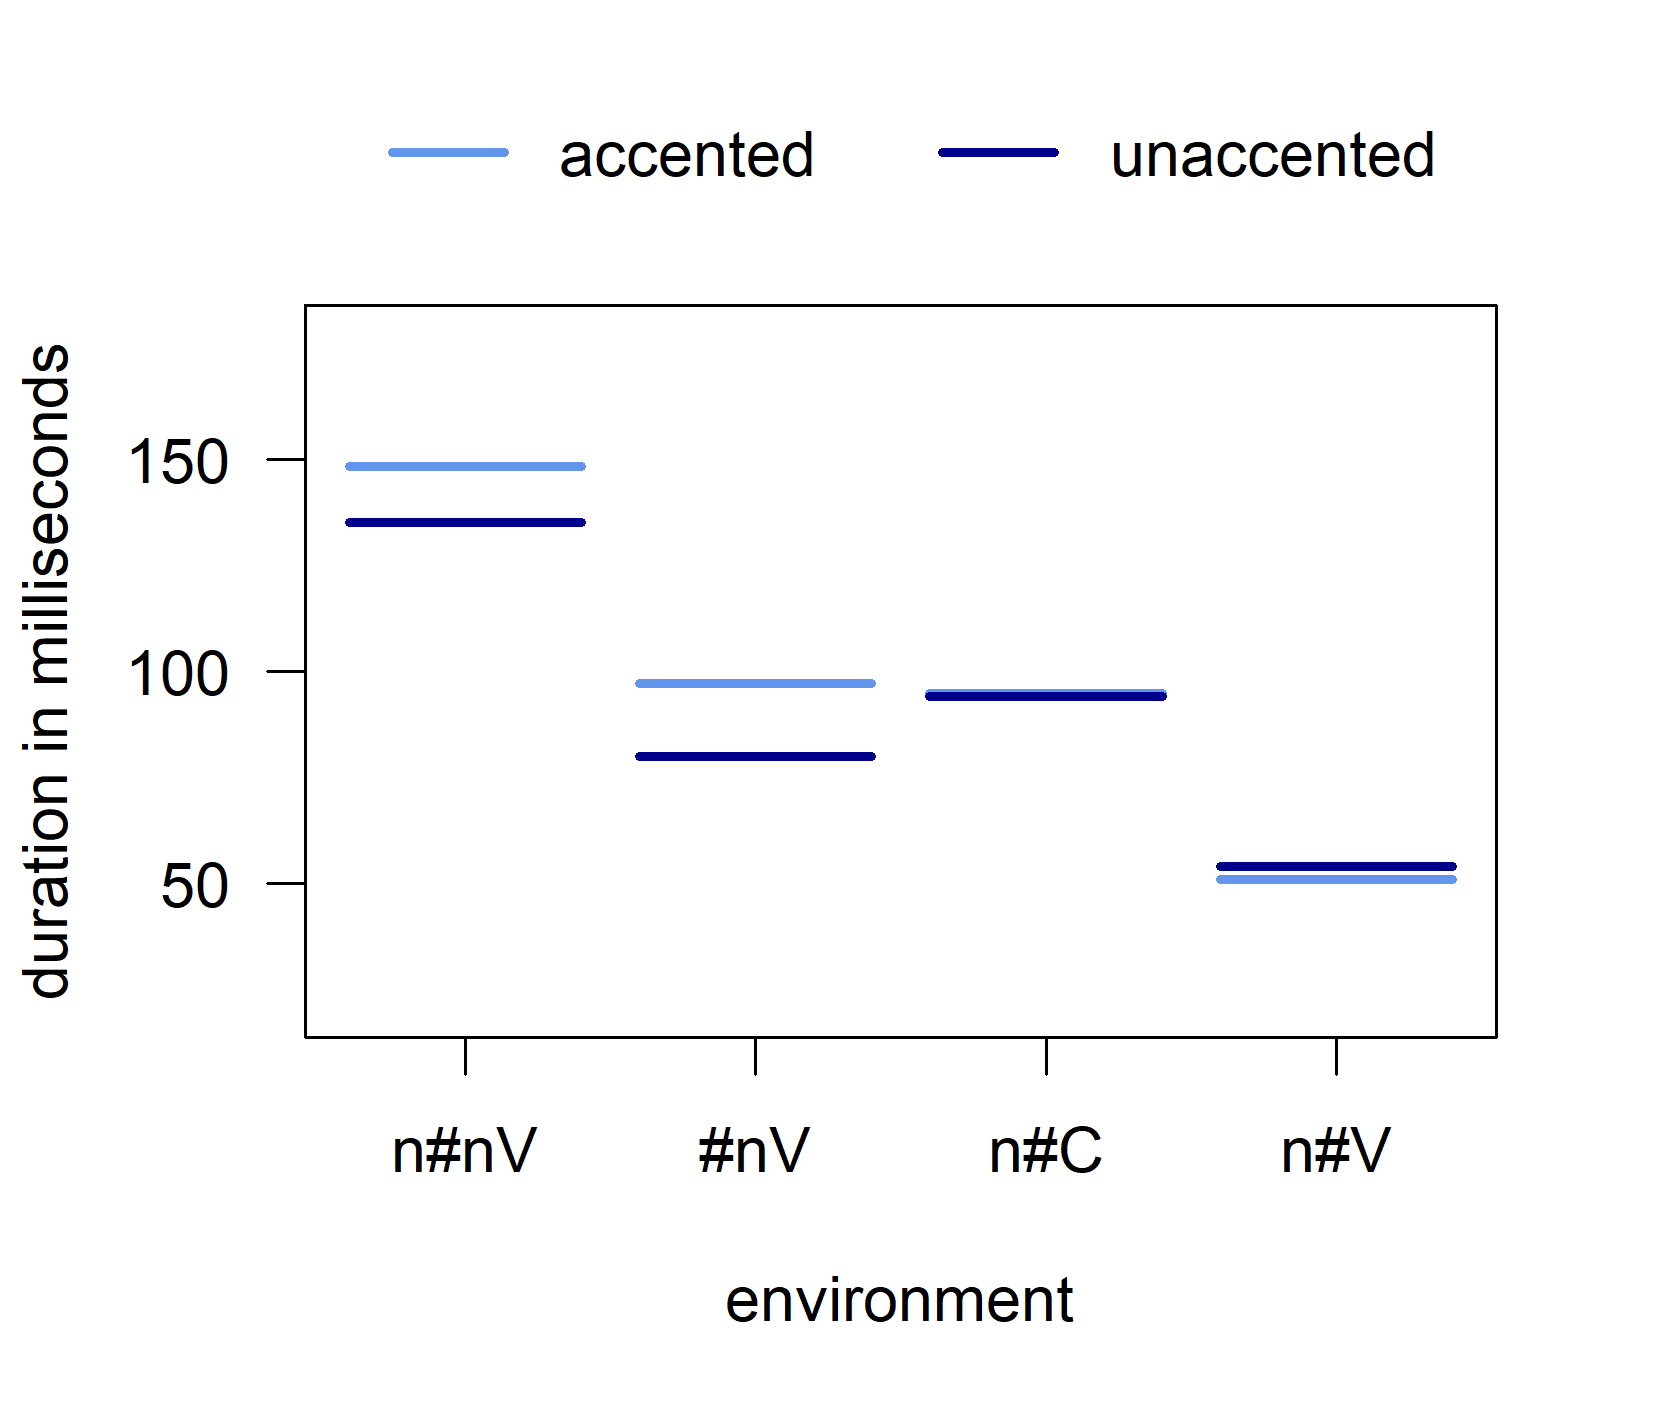
\includegraphics [scale=0.5] {images/Experiment/unModelCompleteInterEnvAcc}
\caption{Effect of accentuation by environment on consonant duration in complete \prefix{un}data set\label{fig:NumNasal Acc un experiment}}
\end{figure*}


 For  doubles (\texttt{n\#nV}) and singletons in base words (\texttt{\#nV}), nasals in \is{accentuation}accented words are longer than nasals in unaccented words.
For singletons in complex words (\texttt{n\#C} and \texttt{n\#V}), consonant duration is not affected by \isi{accentuation}. This has the effect that durational differences between doubles and singletons in complex words are bigger in \is{accentuation}accented than in unaccented position. The durational difference between doubles and singletons in base words is not affected by \isi{accentuation}.

\figref{fig:NumNasal Pauseun experiment} shows the effect of \textsc{PrePause} by \textsc{Environment}. The light blue lines represent the estimated durations for words with no preceding pause, the dark blue lines show the estimated durations for words with a preceding pause. 
The figure shows that all doubles are longer than all types of singletons, i.e. \is{un-}\prefix{un} geminates independent of whether a pause precedes a word or not.
As with \textsc{Accentuation}, only the two environments \texttt{n\#nV} and \texttt{\#nV} are affected by the variable \textsc{PrePause}. For items with a double consonants (\texttt{n\#nV}), the nasal is longer when a pause precedes the word. For base words, the opposite is the case, i.e. the nasal is shorter after a preceding pause.
Crucially, \isi{gemination} does not depend on \textsc{PrePause}. 

\begin{figure*}
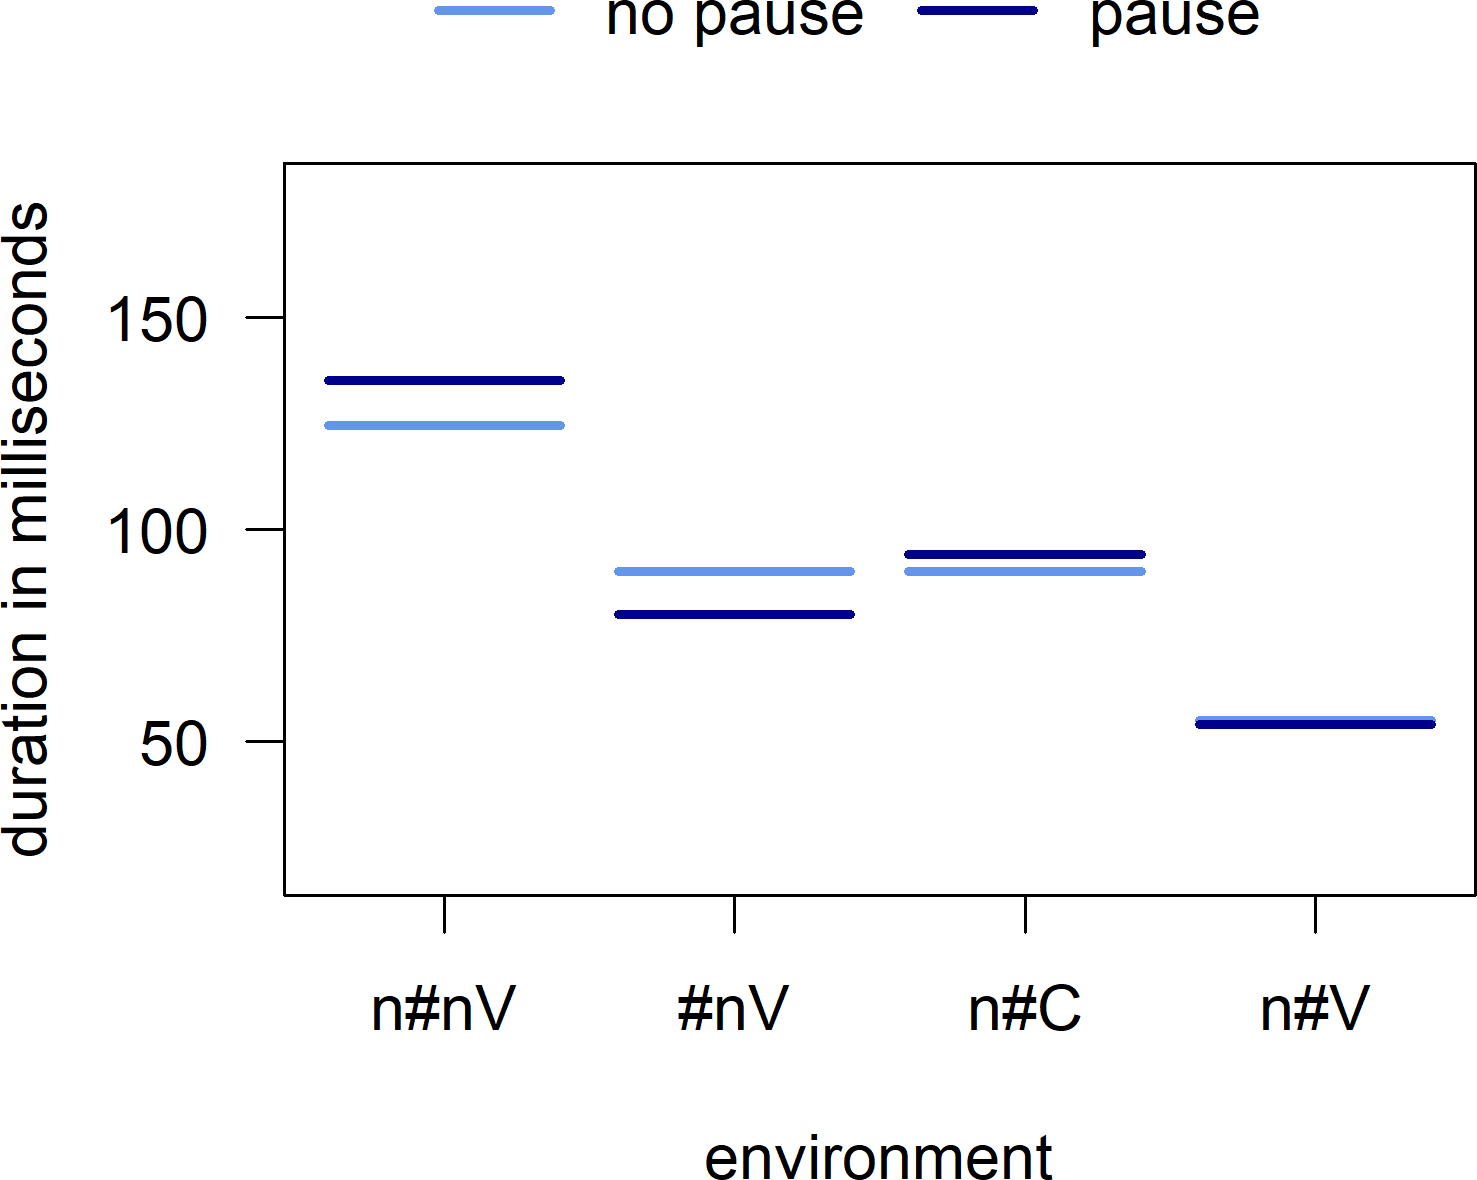
\includegraphics [scale=0.5] {images/Experiment/unModelCompleteInterEnvPause}
\caption{Effect of pause before item by environment on consonant duration in complete \prefix{un}data set}
\label{fig:NumNasal Pauseun experiment}
\end{figure*}


\subsubsection{Summary}


The prefix \is{un-}\prefix{un} clearly geminates. Phonological doubles (\texttt{n\#nV})  are longer than singletons in complex words (\texttt{n\#C}, \texttt{n\#V}) and singletons in base words (\texttt{\#nV}). There are also significant durational differences between the singleton levels with the singletons in base words being the longest, the singletons in prefixed words followed by a consonant being the second longest and the singletons in prefixed words followed by a vowel being the shortest. This pattern resembles the one found in the corpus study. The durational differences between doubles and singletons are, however, much bigger in the experimental study than in the corpus study, i.e. \isi{gemination} seems to be more extreme in the experimental data than in the corpus data. 
As in the corpus study, the \isi{decomposability} measure log\textsc{RelativeFrequency} does not affect nasal duration with \is{un-}\prefix{un}.


 In both \is{un-}\prefix{un}models, the noise variables show the expected effects. In the complex model, the noise variables \textsc{Accentuation}, \textsc{LocalSpeechRate}, \textsc{PrePause} and \textsc{PrecedingSegmentDuration} proved to be significant. In the complete mo-del, the noise variables \textsc{Accentuation}, \textsc{LocalSpeechRate}, \textsc{PrePause} and \textsc{BaseInitialStress} proved to be significant.
 The noise variable \textsc{Accentuation} interacts with the variable \textsc{Environment} in both models. While doubles and singletons in base words are longer when \is{accentuation}accented, singletons in base words are not. In the complete model, there is an interaction between \textsc{PrePause} and \textsc{Environment}. Again, only doubles and singletons in base words are affected by this variable. Crucially,  whether \is{un-}\prefix{un} geminates or not does not depend on \isi{accentuation} or a preceding pause. 


\subsection{The prefix \textit{in-}} \label{in experiment}\largerpage

\subsubsection{The allomorph /ɪn/: Complex model}

The model predicting consonant duration with all complex /ɪn/-words ($N=1232$) was fitted according to the modeling procedure described in \sectref{stats}. Due to an uneven distribution of the residuals in the initial model, the dependent variable \textsc{AbsoluteConsonantDuration} was Box-Cox-transformed ($\lambda = 0.061$) and 22 outliers were removed (1.9\% of the data).
After the model was refitted with the transformed dependent variable, it showed a satisfactory distribution of residuals.  The model was then simplified and interactions were tested (see \hyperref[Appendix G Summaries of tested interactions in experimental study]{Appendix G} for a list of all tested interactions).
The \is{decomposability measure}decomposability variables were tested individually.

The final model features five variables, \textsc{Environment}, \textsc{BaseInitialStress}, \textsc{Accentuation}, \textsc{LocalSpeechRate} and \textsc{PrecedingSegmentDuration}. 
There are two interactions in the model, one between \textsc{Environment} and \textsc{BaseInitialStress}, and one between \textsc{Environment} and \textsc{Accentuation}. The final model is summarized in \tabref{model in complex experiment} in \hyperref[Appendix H: Model Summaries Experiment]{Appendix H}.


The two noise variables \textsc{LocalSpeechRate} and \textsc{PrecedingSegmentDuration} behave as expected. The higher the \isi{speech rate}, the shorter the consonant, and the longer the preceding segment, the shorter the nasal. 


\figref{fig:Env Stress In experiment} shows the interaction between \textsc{BaseInitialStress} and \textsc{Environment}. For each environment, the estimated consonant durations for words with a \is{stress}stressed base-initial syllable are indicated by light blue lines, and the estimated durations for words with an unstressed base-initial syllable are indicated by dark blue lines. 
The plot shows that only when the base-initial syllable of a word is \is{stress}stressed, doubles are predicted to be clearly longer than singletons followed by a vowel (33\,ms). When the base-initial syllable of a word is unstressed, doubles (\texttt{n\#nV}) are predicted to be only 10\,ms longer than singletons followed by a vowel (\texttt{n\#V}).
Doubles are never predicted to be longer than singletons followed by a consonant  (\texttt{n\#C}).
When the base-initial syllable of a word is \is{stress}stressed, doubles are predicted to be as long as singletons followed by a consonant (\texttt{n\#C}). When the base-initial syllable of a word is unstressed, doubles are predicted to be 41\,ms shorter than singletons followed by a consonant (\texttt{n\#C}).




 	\begin{figure*}

 		
 		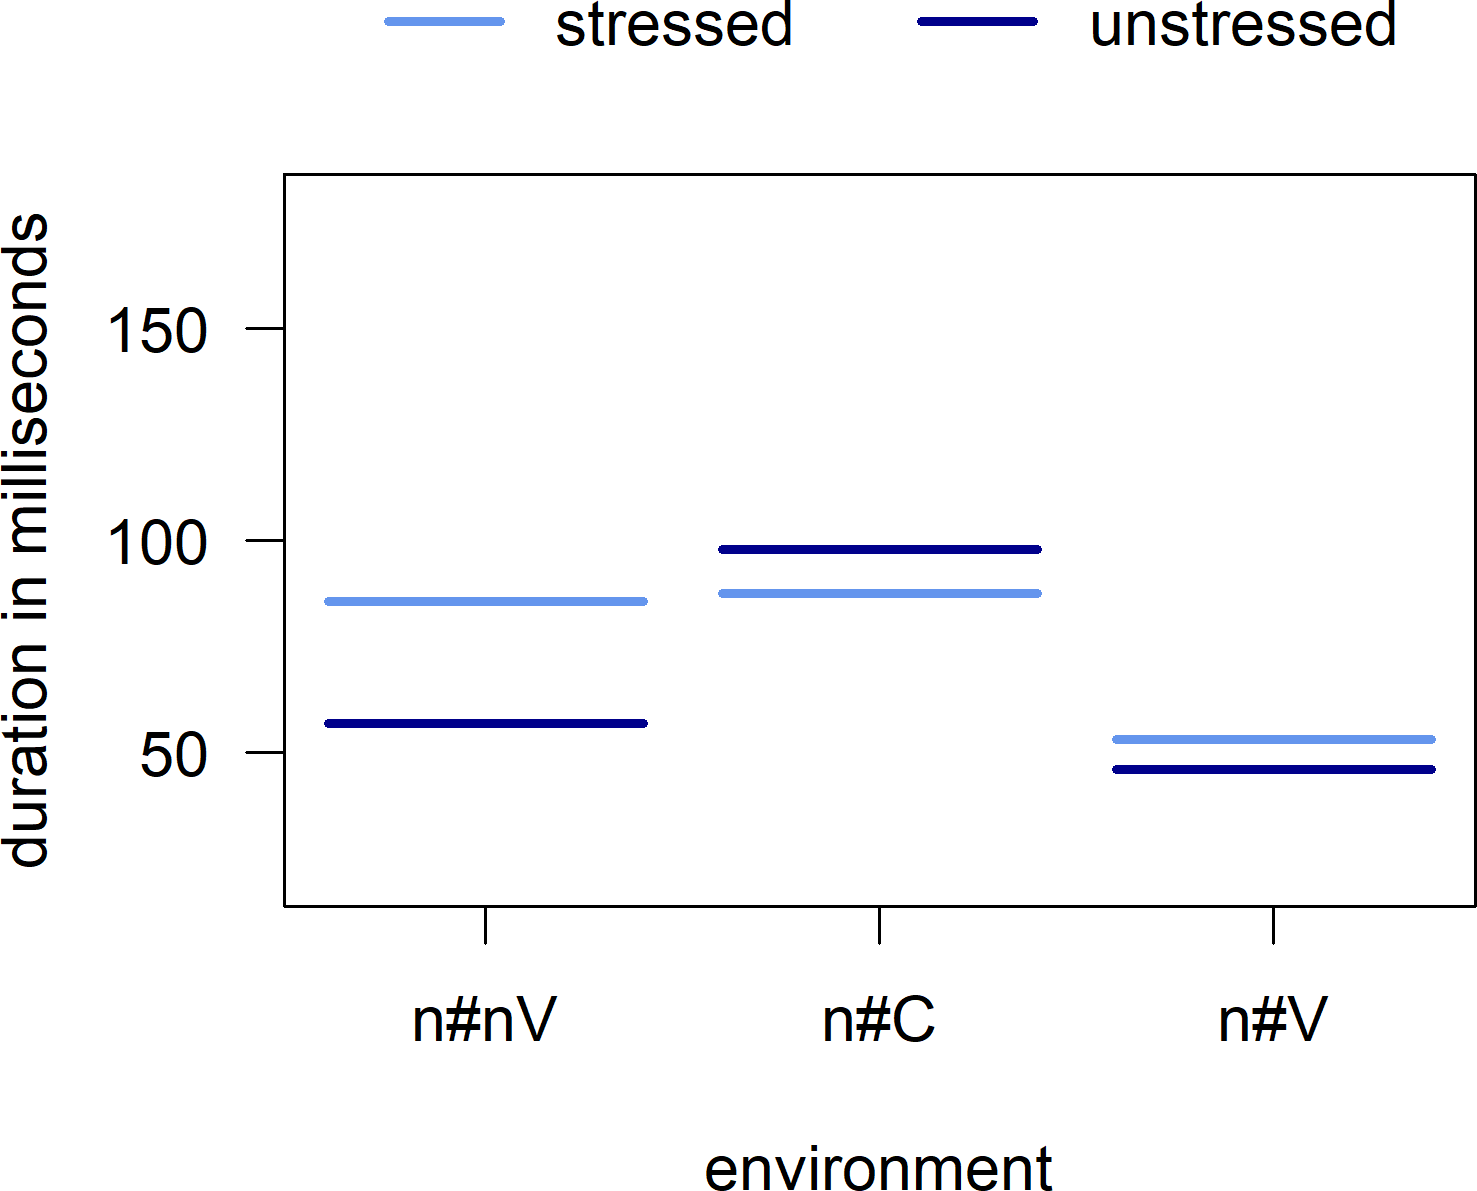
\includegraphics [scale=0.5] {images/Experiment/InModelInterEnvStress}
		
 		\caption{Effect of base-initial stress by environment on consonant duration in complex /ɪn/-data set}		
 		\label{fig:Env Stress In experiment}

 	\end{figure*}%
 	
 	
 

\figref{fig:Env Acc In experiment} shows the interaction between \textsc{Accentuation} and \textsc{Environment}. Light blue lines represent the estimates for \is{accentuation}accented items, and dark blue lines represent the estimated for unaccented items. Note that the figure shows the estimates for items with an unstressed base-initial syllable, and that there is no three-way-interaction between \textsc{BaseInitialStress}, \textsc{Accentuation} and \textsc{Environment}. 


	


	\begin{figure*} 
		
		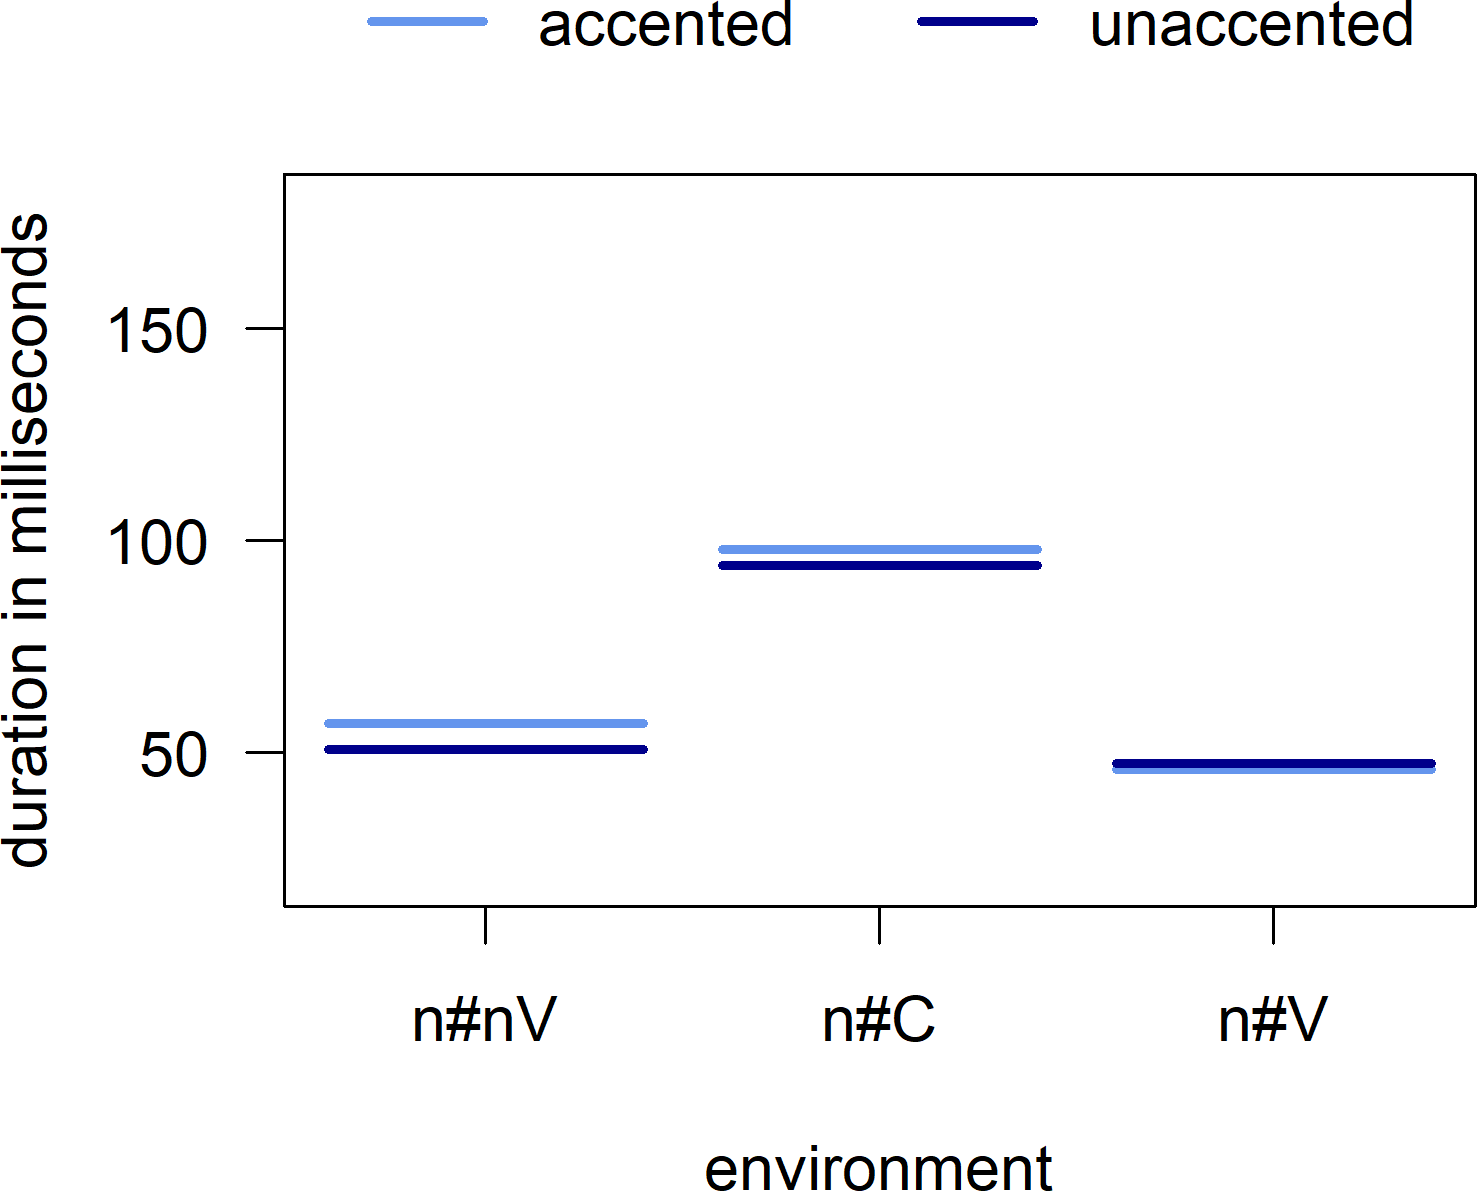
\includegraphics [scale=0.5] {images/Experiment/InModelInterEnvAcc}
		%\vspace*{-0.2cm}
		\caption{Effect of accentuation by environment on consonant duration in complex /ɪn/-data set}
		\label{fig:Env Acc In experiment} 
	\end{figure*}

\largerpage The figure shows that while double consonants (\texttt{n\#nV}) and singletons followed by a consonant (\texttt{n\#C}) are slightly longer when the word is \is{accentuation}accented, singletons followed by a vowel (\texttt{n\#V}) are not affected by \textsc{Accentuation}. Crucially, 
the durational pattern of the three environments does not change depending on whether a word is \is{accentuation}accented or unaccented. 
With unstressed base-initial syllables, singletons followed by a consonant (\texttt{n\#C}) are the longest, followed by doubles (\texttt{n\#nV}), and singletons followed by a vowel (\texttt{n\#V}) are the shortest.
With \is{stress}stressed base-initial syllables, doubles (\texttt{n\#nV}) and singletons followed by a consonant (\texttt{n\#C}) are of the same duration, and singletons followed by a vowel (\texttt{n\#V}) are shorter.\footnote{Note that the durational differences for words with \is{stress}stressed base-initial syllables cannot be seen in \figref{fig:Env Acc In experiment}.}


%AIC

The effect size of each significant term in the model is displayed in \figref{fig:Effect sizes InComplex Exp}. As in the \is{un-}\prefix{un}model, the variables \textsc{Speaker}, \textsc{Environment}, \textsc{LocalSpeechRate} and \textsc{Item} explain most of the variance found in the data. Crucially, the variable \textsc{Environment} is very important for the model, i.e. the number of consonants at the morphological boundary, as well as the segment following the nasal, highly influence the duration of the nasal. In contrast to \is{un-}\prefix{un}, \textsc{Environment} does, however, not explain most of the variance found in the data. It thus seems that it is less important for predicting consonant duration with /ɪn/-prefixed words than with \is{un-}\prefix{un}prefixed words. 





%PC Model

None of the \is{decomposability measure}decomposability measures proved to be significant in the final model. On the one hand, this might mean that \isi{decomposability} does not affect consonant duration with /ɪn/. On the other, there is the possibility that the individual \is{decomposability measure}decomposability measures are not strong enough to reach significance on their own. As a combined \isi{decomposability} measure, they might, however, become significant in the model (see also discussions in Sections~\ref{analsyses duration experiment} and~\ref{in corpus}).





\begin{figure*}
	
	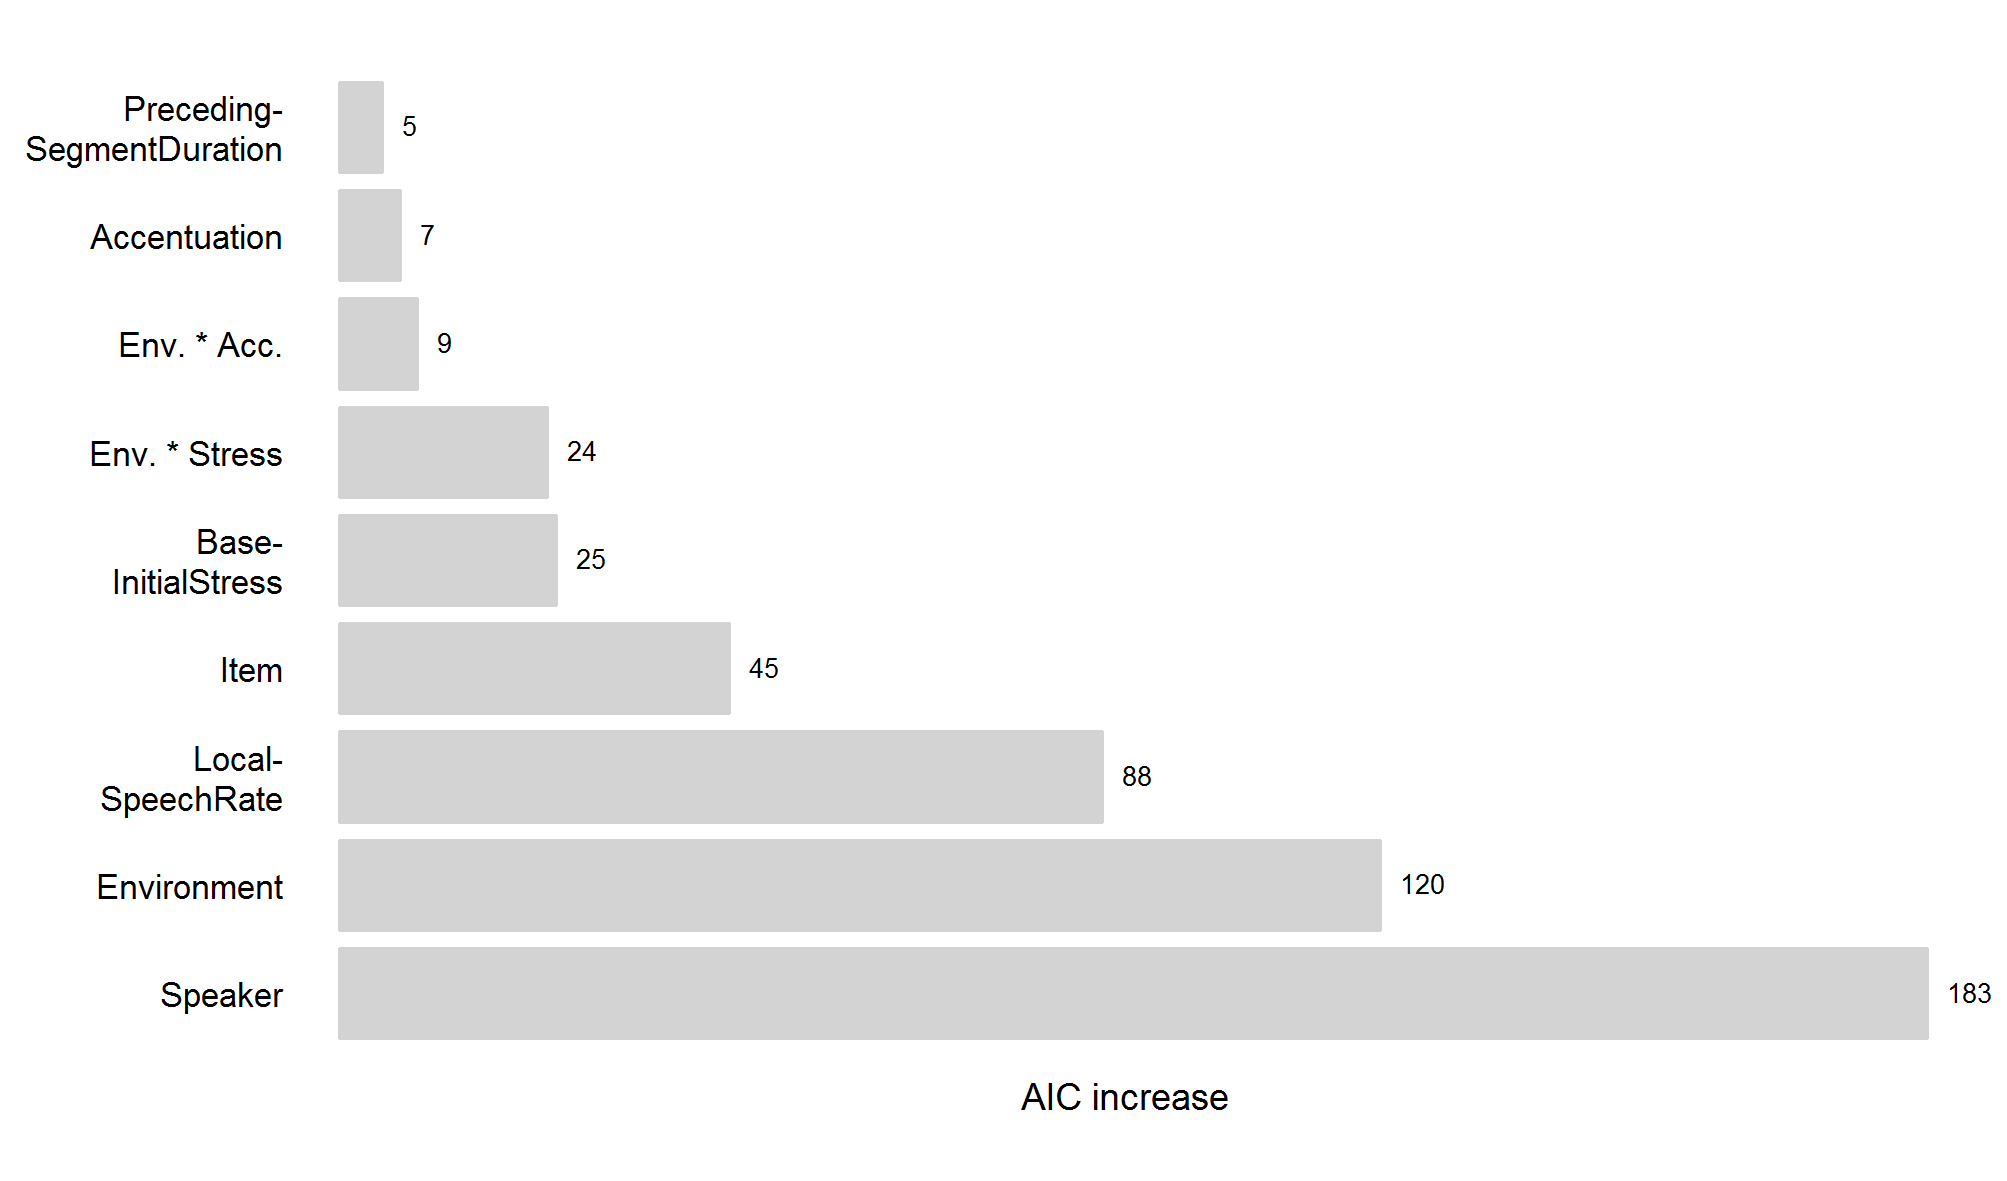
\includegraphics[scale=0.7]{images/Experiment/AICdecreaseInComplex.png}
	
	\caption{AIC increase for each variable of the final /ɪn/-model, AIC final model = -6974}
	\label{fig:Effect sizes InComplex Exp}
	
\end{figure*}


To test this idea, an additional model with combined \is{decomposability measure}decomposability measures (as opposed to individual \is{decomposability measure}decomposability measures) was fitted. The combined measures were created by means of a \is{principal component analysis}principal component analysis (see \sectref{stats} on \is{principal component analysis}principal component analyses). 
As in the corpus study, the \is{principal component analysis}principal component analysis was fitted with the variables log\textsc{RelativeFrequency}, \textsc{SemanticTransparency}, \textsc{SemanticTransparencyRating}, \textsc{TypeOfBase} and \textsc{Affix}. The variable \textsc{Affix} features the two levels \texttt{inLoc} (\is{locative in-}locative \prefix{in}) and \texttt{inNeg} (\is{negative in-}negative \prefix{in}). All variables were recoded into numerical variables and scaled before the analysis was conducted. 
\tabref{tbl: summary PC in exp} summarizes the analysis by showing the composition of each \is{principal component analysis}principal component, i.e. the loading of each variable for each \is{principal component analysis}principal component, and by displaying the proportion of variance covered by each component. 










The \is{principal component analysis}principal component analysis revealed that the first three components can account for most of the variance expressed by the five \is{decomposability measure}decomposability variables (90\%). An inspection of the rotation matrix shows that the first component is composed of all five measures, that the second is mainly dominated by the variables scaled\textsc{Affix} and scaled\textsc{RelativeFrequency}, and that the third is mainly dominated by the variable scaled\textsc{SemanticTransparencyRating}. 
The first three principal components were included as predictor variables in the mixed model.  




\begin{table*}
	\caption{Summary of principal components\label{tbl: summary PC in exp}}
	\resizebox{\textwidth}{!}{%		
		\begin{tabular}{l *{5}{S[table-format=+1.3]}}
			\lsptoprule
			 &  {PC1} &   {PC2} &  {PC3} & {PC4} & {PC5}  \\
			\midrule
			\multicolumn{6}{l}{Composition of principal components}\\
			\midrule
				scaled\textsc{Affix} & -0.457 & 0.591 & 0.022 & -0.324 & -0.580 \\
				scaled\textsc{RelativeFrequency}  &  -0.390 & -0.724 & -0.347 & -0.391 & -0.225 \\ 
				scaled\textsc{SemanticTransparencyRating}  &-0.391 & -0.252 & 0.882 & 0.036 & 0.065 \\ 
				scaled\textsc{TypeOfBase}& -0.469 & -0.037 & -0.242 & 0.836 & -0.145 \\ 
				scaled\textsc{SemanticTransparency} & -0.516 & 0.250 & -0.206 & -0.205 & 0.767 \\ 		
			\midrule
			\multicolumn{6}{l}{Variance explained by principal components}\\
			\midrule
				Proportion of Variance &0.626& 0.150& 0.121 & 0.076& 0.027\\
				\lspbottomrule
			\end{tabular}}
\end{table*}

The model was fitted similarly to the model with the individual \is{decomposability measure}decomposability measures. After model simplification, none of the principal components remained in the model. This means, the simplification of the model resulted in the same final model as the simplification of the model with the individual \is{decomposability measure}decomposability measures. Decomposability does not affect consonant duration with /ɪn/.




To sum up, the analyses have shown that prefixal nasal duration in /ɪn/- prefixed words is influenced by the variables \textsc{Environment}, \textsc{BaseInitialStress}, \textsc{Accentuation}, \textsc{LocalSpeechRate} and \textsc{PrecedingSegmentDuration}. None of the \is{decomposability measure}decomposability variables influences nasal duration with /ɪn/, neither as independent measures nor as combined measures. 
While the noise variables \textsc{Accentuation}, \textsc{LocalSpeechRate} and \textsc{PrecedingSegmentDuration} behave as expected and do not influence the \isi{gemination} pattern of /ɪn/, the variable \textsc{BaseInitialStress} affects \isi{gemination} with /ɪn/. 
Only when the base-initial syllable of a prefixed word is \is{stress}stressed, double consonants (\texttt{n\#nV}) are predicted to be clearly longer than singletons with a following vowel (\texttt{n\#V}). In this case, i.e. when the base-initial syllable is \is{stress}stressed, doubles are predicted to be as long as singletons followed by a consonant (\texttt{n\#C}). When the base-initial syllable of a word is unstressed, doubles (\texttt{n\#nV} ) are predicted to be only marginally longer than singletons with a following vowel (\texttt{n\#V}). In this case, they are predicted to be shorter than singletons followed by a consonant (\texttt{n\#C}).

\subsubsection{The allomorph /ɪn/: Complete model}\largerpage
The model predicting consonant duration with all /ɪn/-words ($N=1232$) was fitted according to the modeling procedure described in \sectref{stats}. Due to an uneven distribution of the residuals in the initial model, the dependent variable \textsc{AbsoluteConsonantDuration} was Box-Cox-transformed ($\lambda = 0.202$) and 22 outliers were removed (1.79\% of the data). 
After the transformation, the model showed a satisfactory distribution of residuals. The model was then simplified and interactions were tested (see \hyperref[Appendix G Summaries of tested interactions in experimental study]{Appendix G} for a list of all tested interactions).

The final model features the five variables \textsc{LocalSpeechRate}, \textsc{Environment}, \textsc{BaseInitialStress}, \textsc{Accentuation} and \textsc{PrePause} (see \tabref{model in complete experiment} in \hyperref[Appendix H: Model Summaries Experiment]{Appendix H} for a summary of the final complete model). 
The noise variable \textsc{LocalSpeech\-Rate} shows the expected effect. The other three noise variables interact with the variable \textsc{Environment}, i.e. there are three two-way interactions in the model, one between \textsc{BaseInitialStress} and \textsc{Environment}, one between \textsc{Accentuation} and \textsc{Environment}, and one between \textsc{PrePause} and \textsc{Environment}.  Note that all pertinent three-way interactions were tested but none proved to be significant.


	\begin{figure*}
		 
		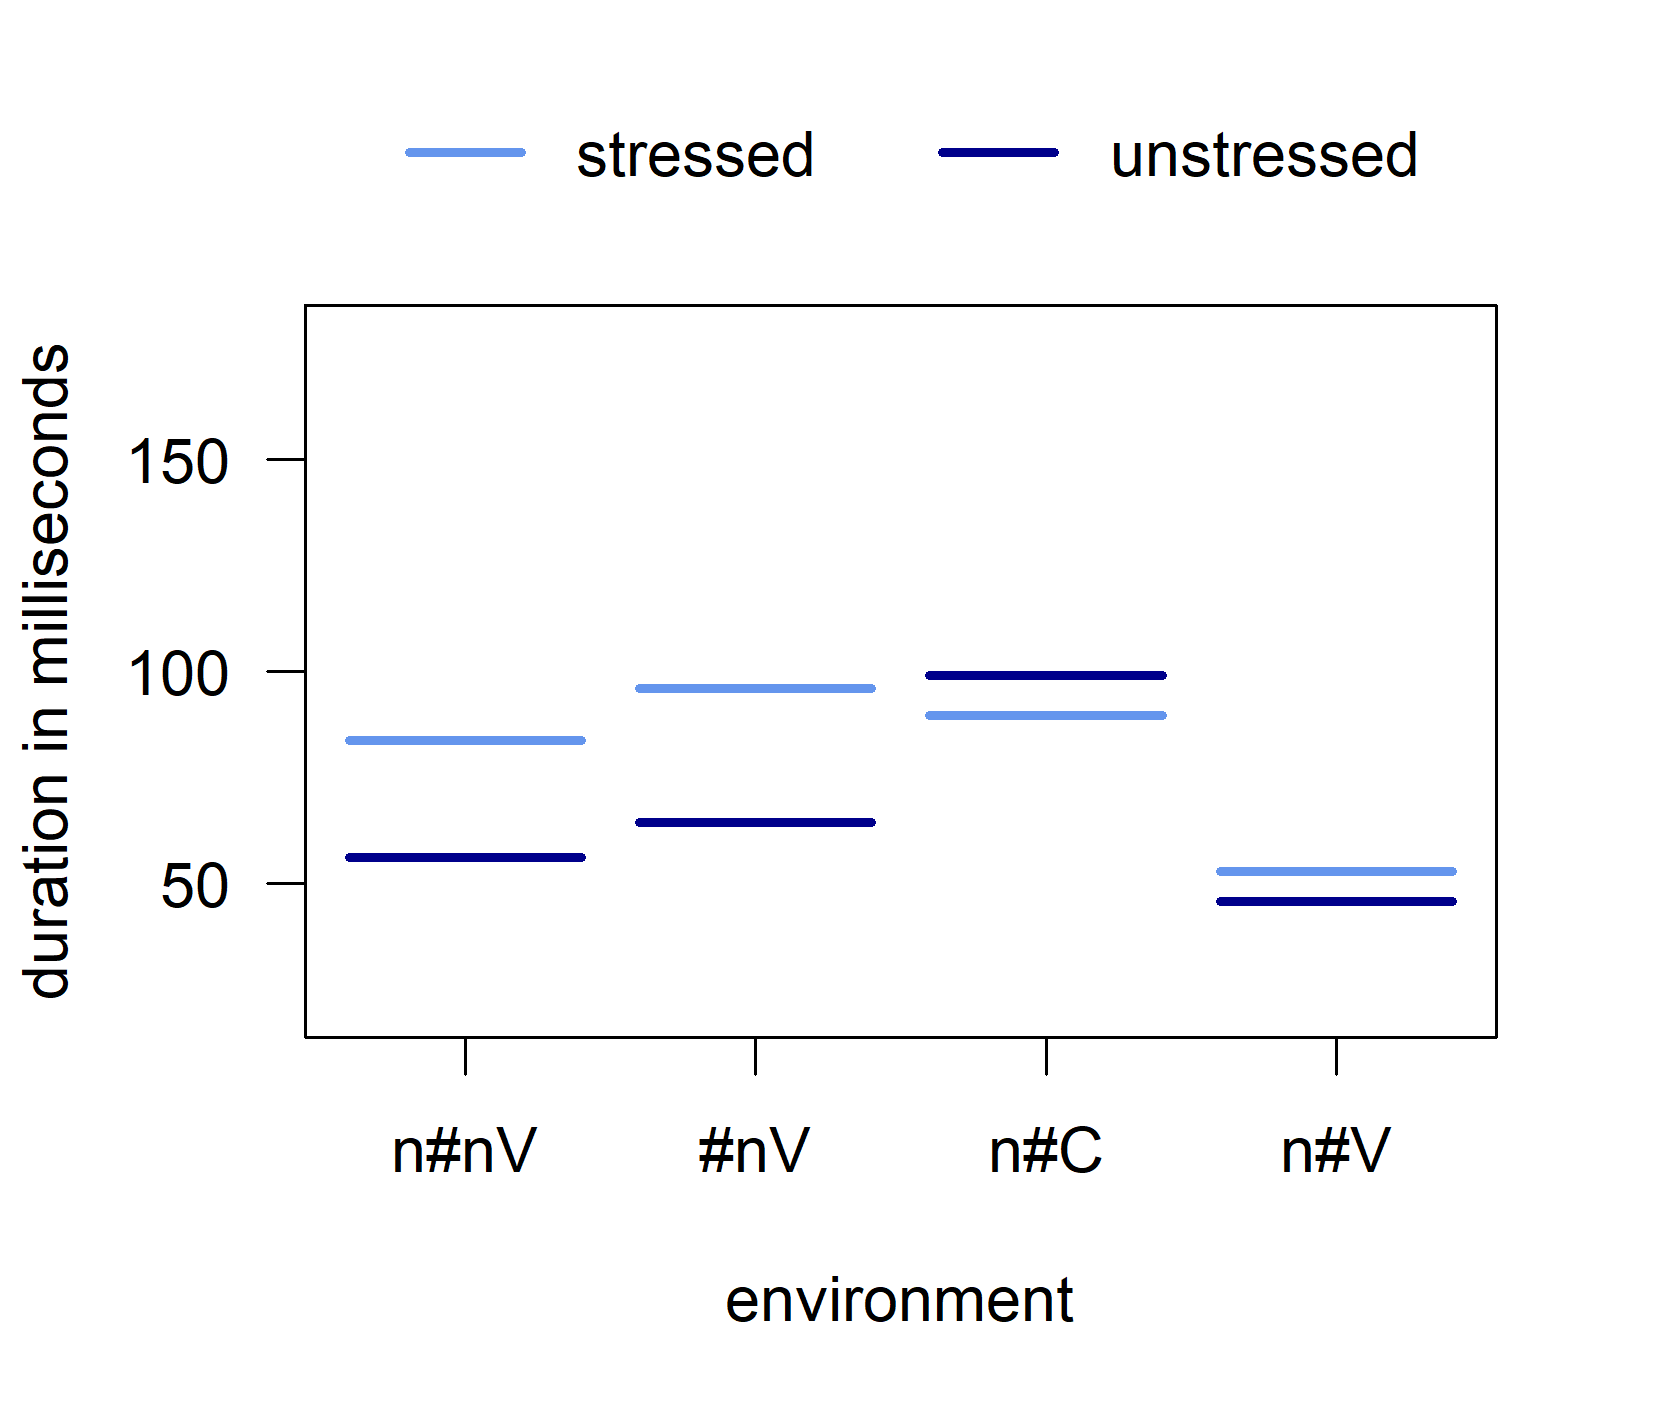
\includegraphics [scale=0.5] {images/Experiment/InModelCompleteInterEnvStress}
		
		\caption{Effect of base-initial stress by environment on consonant duration in /ɪn/-data set}	
		\label{fig:Env Stress In complete experiment} 
	\end{figure*}%








%\isi{stress}
\figref{fig:Env Stress In complete experiment} shows the effect of \textsc{BaseInitialStress} on \textsc{Environment}. Light blue lines indicate estimates for words with \is{stress}stressed base-initial syllables, and dark blue lines indicate estimates for words with unstressed base-initial syllables. The plot shows the predicted durations for \is{accentuation}accented items.



As the complex /ɪn/-model, the complete model reveals that \isi{stress} affects \isi{gemination} with /ɪn/. 
The plot shows that only when doubles (\texttt{n\#nV}) are part of a word with a \is{stress}stressed base-initial syllable, they are as long as singletons with a following consonant  (\texttt{n\#C}) and longer than singletons with a following vowel  (\texttt{n\#V}). When part of a word with an unstressed base-initial syllable, doubles are shorter than singletons followed by a consonant and only slightly longer than singletons followed by a vowel. Independent of \textsc{BaseInitialStress}, doubles are slightly shorter than singletons in base words.




%Acentuation
\figref{fig:Env Acc In complete experiment} shows the interaction between \textsc{Accentuation} and \textsc{Environment}. Estimates for \is{accentuation}accented items are indicated by light blue lines, estimates for unaccented items by dark blue lines. The figure shows the estimates for words with an unstressed base-initial syllable. 


	\begin{figure*}
		
		
		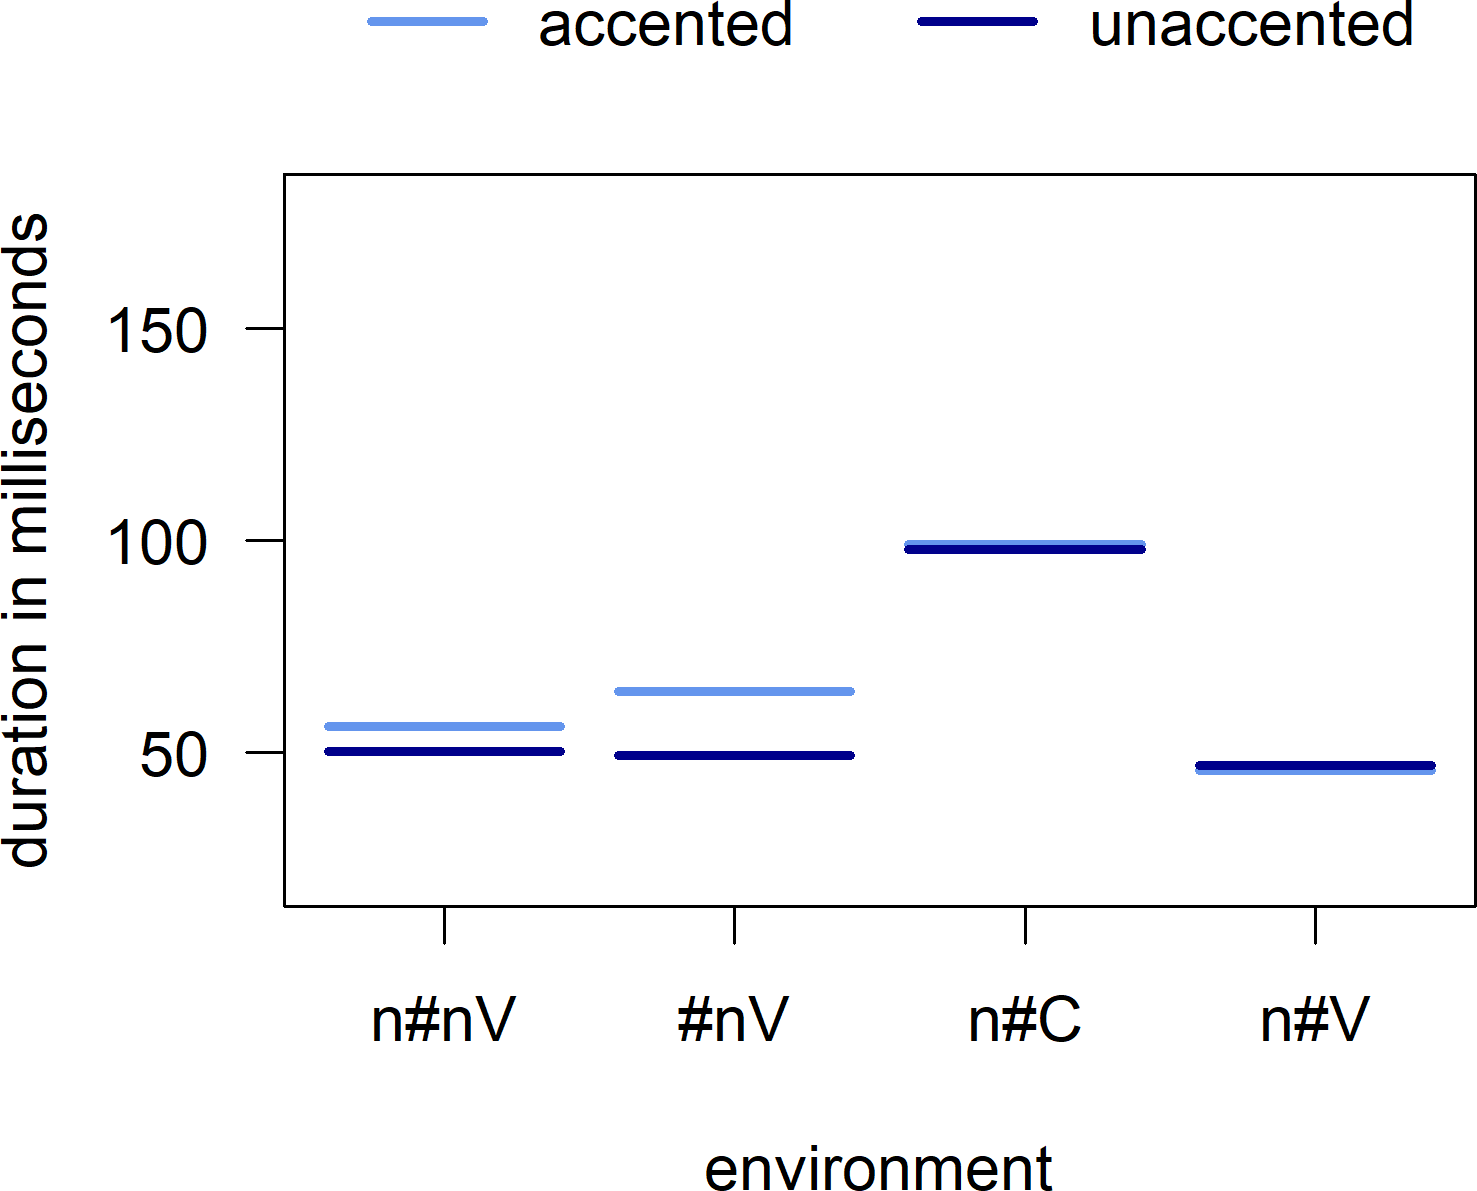
\includegraphics [scale=0.5] {images/Experiment/InModelCompleteInterEnvAcc} 
		\caption{Effect of accentuation by environment on consonant duration in /ɪn/-data set}
		\label{fig:Env Acc In complete experiment}
	\end{figure*}

\largerpage The plot shows that only the durational pattern of doubles and singletons in base words is affected by \isi{accentuation}. 
In unaccented condition, singletons in base words and doubles are of the same duration. In \is{accentuation}accented condition, singletons in base words are longer. Crucially, doubles are never longer than singletons in base words.
The durational pattern of doubles and singletons in complex words is not affected by \isi{accentuation}. For words with an unstressed base-initial syllable, doubles are shorter than singletons followed by a consonant, and slightly longer than singletons followed by a vowel. For words with a \is{stress}stressed base-initial syllable, doubles are as long as singletons followed by a consonant and longer than singletons followed by a vowel.\footnote{Note that the durational differences for words with \is{stress}stressed base-initial syllables cannot be seen in \figref{fig:Env Acc In complete experiment}.} 


%PrePause

\figref{fig:Env Pause In complete experiment} shows the interaction between \textsc{PrePause} and \textsc{Environment}. Light blue lines indicate the estimated nasal durations for words with no preceding pause, and dark blue lines show the estimated nasal durations for words with a preceding pause.
The figure shows that only the duration of singletons in base words (\texttt{\#nV}) is affected by a preceding pause. When a pause precedes a base word, nasals are shorter than when there is no preceding pause. This effect was also observed with \is{un-}\prefix{un}, and is therefore not surprising. 
The effect of \textsc{PrePause} does not affect \isi{gemination} with /ɪn/.



\begin{figure*}
	
	
	
	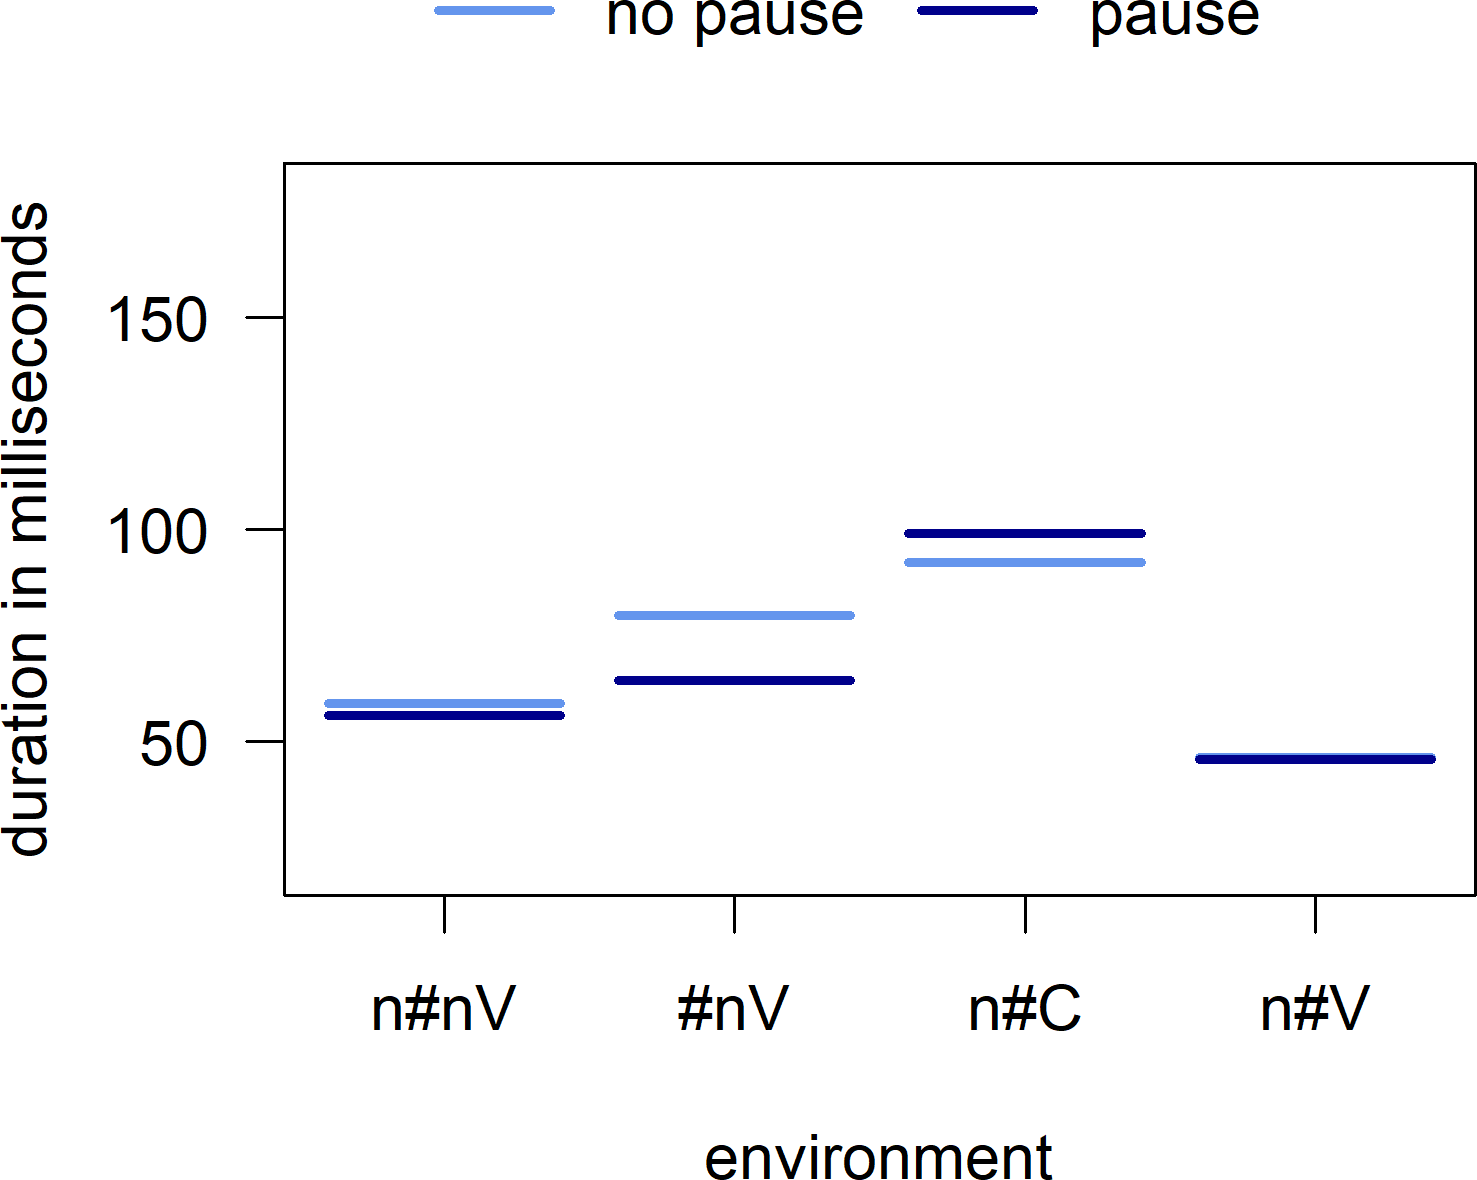
\includegraphics [scale=0.5] {images/Experiment/InModelCompleteInterEnvPause}
	\caption{Effect of pause before item by environment on consonant duration in /ɪn/-data set}
	\label{fig:Env Pause In complete experiment}
\end{figure*}	




As with the complex model, the results of the complete /ɪn/-model show that only when the base-initial syllable of a complex word is \is{stress}stressed, phonological doubles with /ɪn/ are longer than singletons in complex words followed by a vowel. 
Phonological doubles are never longer than singletons in complex words followed by a consonant or singletons in base words. 
This suggests that \isi{gemination} with \is{in-}\prefix{in} depends on the stress-pattern of the prefixed word.  Only when the base-initial syllable of a double-consonant word is \is{stress}stressed, the prefix geminates. It, furthermore, suggests that \isi{gemination} with \is{in-}\prefix{in} is weaker than \isi{gemination} with \is{un-}\prefix{un}.


In contrast to morphological geminates with \is{un-}\prefix{un}, 
morphological geminates with /ɪn/ are not longer than all types of singletons, i.e. they are not longer than singletons in base words and they are not longer than singletons in prefixed words followed by a consonant. 
That doubles with /ɪn/ are not longer than singletons followed by a consonant could be attributed to a lengthening effect caused by the following consonant.
It is expected that nasals followed by a consonant are longer than nasals followed by a vowel (see, for example, \citealt{Umeda.1977}, see also discussion in \sectref{variables of interest}).  Thus, singletons followed by a consonant might only be as long as doubles because they are lengthened by the following consonant. However, for \is{un-}\prefix{un} this lengthening effect did not result in a lack of durational difference between doubles and singletons followed by a consonant, but only in smaller durational differences between doubles and singletons.  

That \is{un-}\prefix{un} geminates to a higher degree than \is{in-}\prefix{in} is also suggested by the fact that the durational differences between doubles and singletons for /ɪn/ are much smaller than the ones for \is{un-}\prefix{un} (\isi{singleton-geminate ratio} for \is{un-}\prefix{un}: 1:3.0, \isi{singleton-geminate ratio} for /ɪn/: 1:1.6). 
The AIC increase analysis also supports the idea that \isi{gemination} is less strong with /ɪn/. It revealed that the variable \textsc{Environment} is of less importance in the /ɪn/-model than in the \is{un-}\prefix{un}model.




However, before coming to a conclusion with regard to the \isi{gemination} pattern of \is{in-}\prefix{in}, one must take a few additional facts into consideration. 
First, there are only four types of /ɪn/-prefixed words with a double consonant in the data set (\textit{innervate}, \textit{innocuous}, \textit{innominate}, \textit{innumerable}). Three of them feature a \is{stress}stressed base-initial syllable. This means that there is only one /ɪn/-prefixed type that does not geminate. It seems rather bold to make generalizations based on this one type. 
Second, as /ɪn/ is only one of several allomorphs of the prefix \is{in-}\prefix{in}, and as the \isi{gemination} of the prefix \is{in-}\prefix{in} is expected to follow similar patterns across allomorphs, 
a final conclusion with regard to the \isi{gemination} pattern of \is{in-}\prefix{in} can only be drawn after more empirical facts are revealed, i.e. after the results of the \is{im-}/ɪm/-models are discussed.


\subsubsection{The allomorph /ɪm/: Complex model}


%Intro
The model predicting consonant duration with all complex \is{im-}/ɪm/-words ($N=1177$) was fitted according to the modeling procedure described in \sectref{stats}.
Because the initial model showed a non-normal distribution,  24 outliers (2.04\% of the data) were removed and the dependent variable was Box-Cox-transformed ($\lambda = 0.101$).  
After the model was refitted with the transformed dependent variable, it showed a satisfactory distribution of residuals. The model was then simplified and interactions were tested (see \hyperref[Appendix G Summaries of tested interactions in experimental study]{Appendix G} for a list of all tested interactions). 
The \is{decomposability measure}decomposability variables were tested individually.\pagebreak



%Covariates
The final model features five variables, \textsc{Environment}, \textsc{BaseInitialStress}, \textsc{Accentuation}, \textsc{LocalSpeechRate} and \textsc{GlobalSpeechRate}. There are two interactions in the model, one between \textsc{BaseInitialStress} and \textsc{Accentuation}, and one between \textsc{BaseInitialStress} and \textsc{Environment}. The model is shown in \tabref{model im complex experiment} in \hyperref[Appendix H: Model Summaries Experiment]{Appendix H}.

The two noise variables \textsc{LocalSpeechRate} and \textsc{GlobalSpeechRate} show the expected effects. With increasing \isi{speech rate}, the nasal becomes shorter.
 The other two noise variables \textsc{BaseInitialStress} and \textsc{Accentuation} interact. In \is{accentuation}accented position, nasals are longer when the base-initial syllable of a word is \is{stress}stressed. In unaccented position, the opposite is the case, i.e. words with an unstressed base-initial syllable feature longer nasals than words with a \is{stress}stressed base-initial syllable. 
 


%Effect Environment
As in the /ɪn/-models, the variable of interest \textsc{Environment} interacts with \textsc{BaseInitialStress}. The effect is shown in \figref{fig:NumNasal imComplex experiment}. 
The light blue lines represent the estimated nasal durations for items with a \is{stress}stressed base-initial syllable, the dark blue lines represent  the estimated durations for items with an unstressed base-initial syllable.
The figure clearly shows that 
 only when the base-initial syllable is \is{stress}stressed, doubles are  longer than singletons. When the base-initial syllable is unstressed, doubles are shorter than singletons. 
Thus, as with /ɪn/, \isi{gemination} seems to depend on the \isi{stress} status of the base-initial syllable of a word. Only when it is \is{stress}stressed, the prefix \is{in-}\prefix{in} geminates.

 \begin{figure*}
 	
 	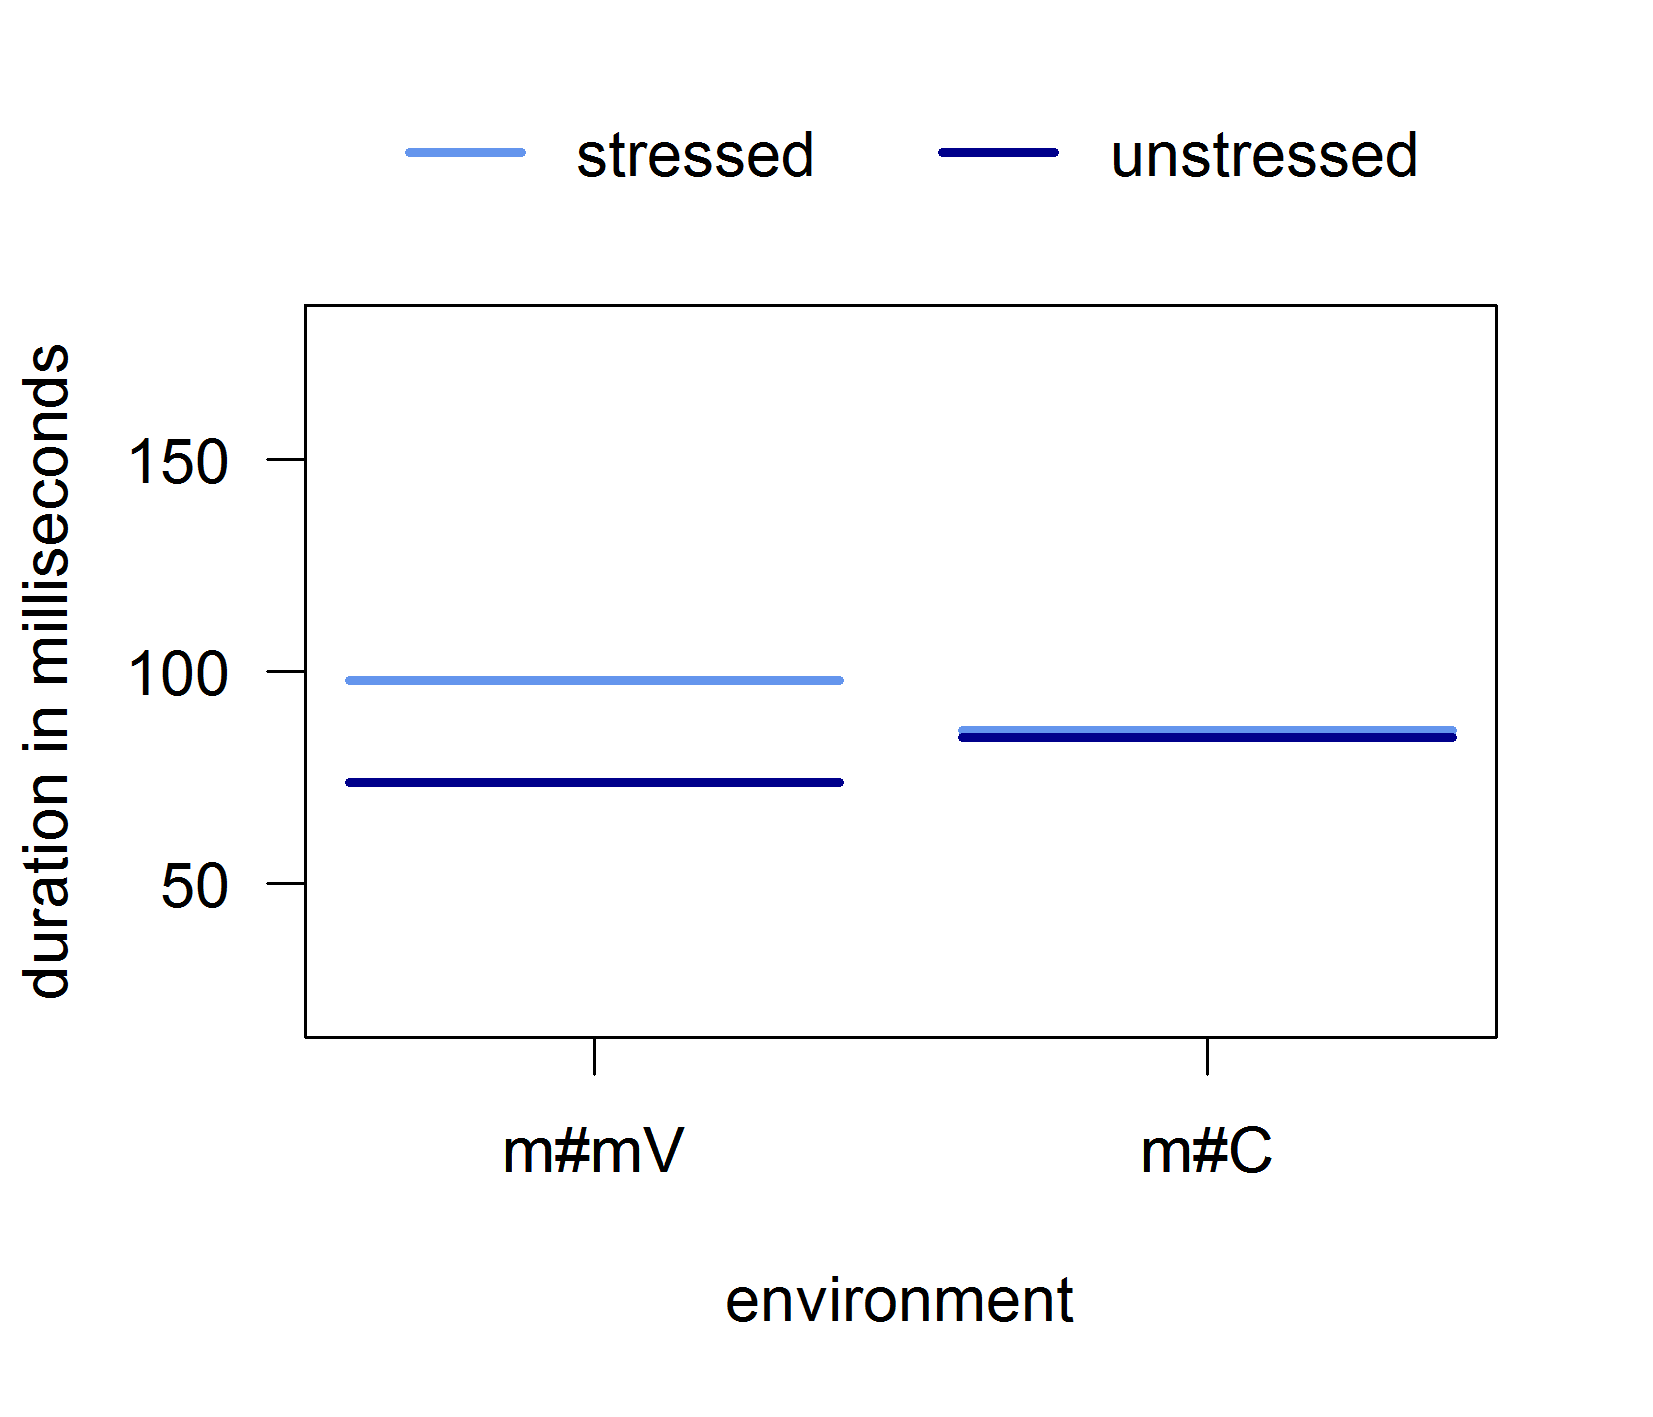
\includegraphics [scale=0.5] {images/Experiment/imModelInterEnvStress}
 	\caption{Effect of base-initial stress by environment on consonant duration in complex /ɪm/-data set}
 	\label{fig:NumNasal imComplex experiment}
 	
 \end{figure*}



The durational differences between doubles and singletons are rather small.  When the base-initial syllable is \is{stress}stressed, doubles are 12\,ms longer than singletons. When the base-initial syllable is unstressed, doubles are 10\,ms shorter than singletons. 
  One could explain these small differences by referring to the difference in the following segment between doubles and singletons in the \is{im-}/ɪm/ -data set. Doubles are always followed by a vowel, and singletons are always followed by a consonant. As shown in the corpus and the experimental study with \is{un-}\prefix{un} and /ɪn/, following vowels shorten the preceding nasal, i.e. the double, and following consonants lengthen the preceding nasal, i.e. the singleton. One might thus suspect that if one kept the environment constant for doubles and singletons, the durational difference between doubles and singletons in words with a \is{stress}stressed base-initial syllable would be larger, and doubles in words with an unstressed base-initial syllable would not be shorter than singletons. 

However, if one compares the results with the ones of the \is{im-}/ɪm/ -corpus study, one can see that the durational difference between doubles and singletons followed by a consonant was much larger in the corpus study (27\,ms). Furthermore, in the corpus study \isi{gemination} was not dependent on the \isi{stress} status of the base-initial syllable.
It thus seems that \isi{gemination} with \is{im-}/ɪm/  differs between corpus and experimental data. In the corpus, \isi{gemination} with \is{im-}/ɪm/  is stronger and independent of prosodic factors, whereas in the experimental data \isi{gemination} is weaker and depends on base-initial \isi{stress}.


\begin{figure*}
	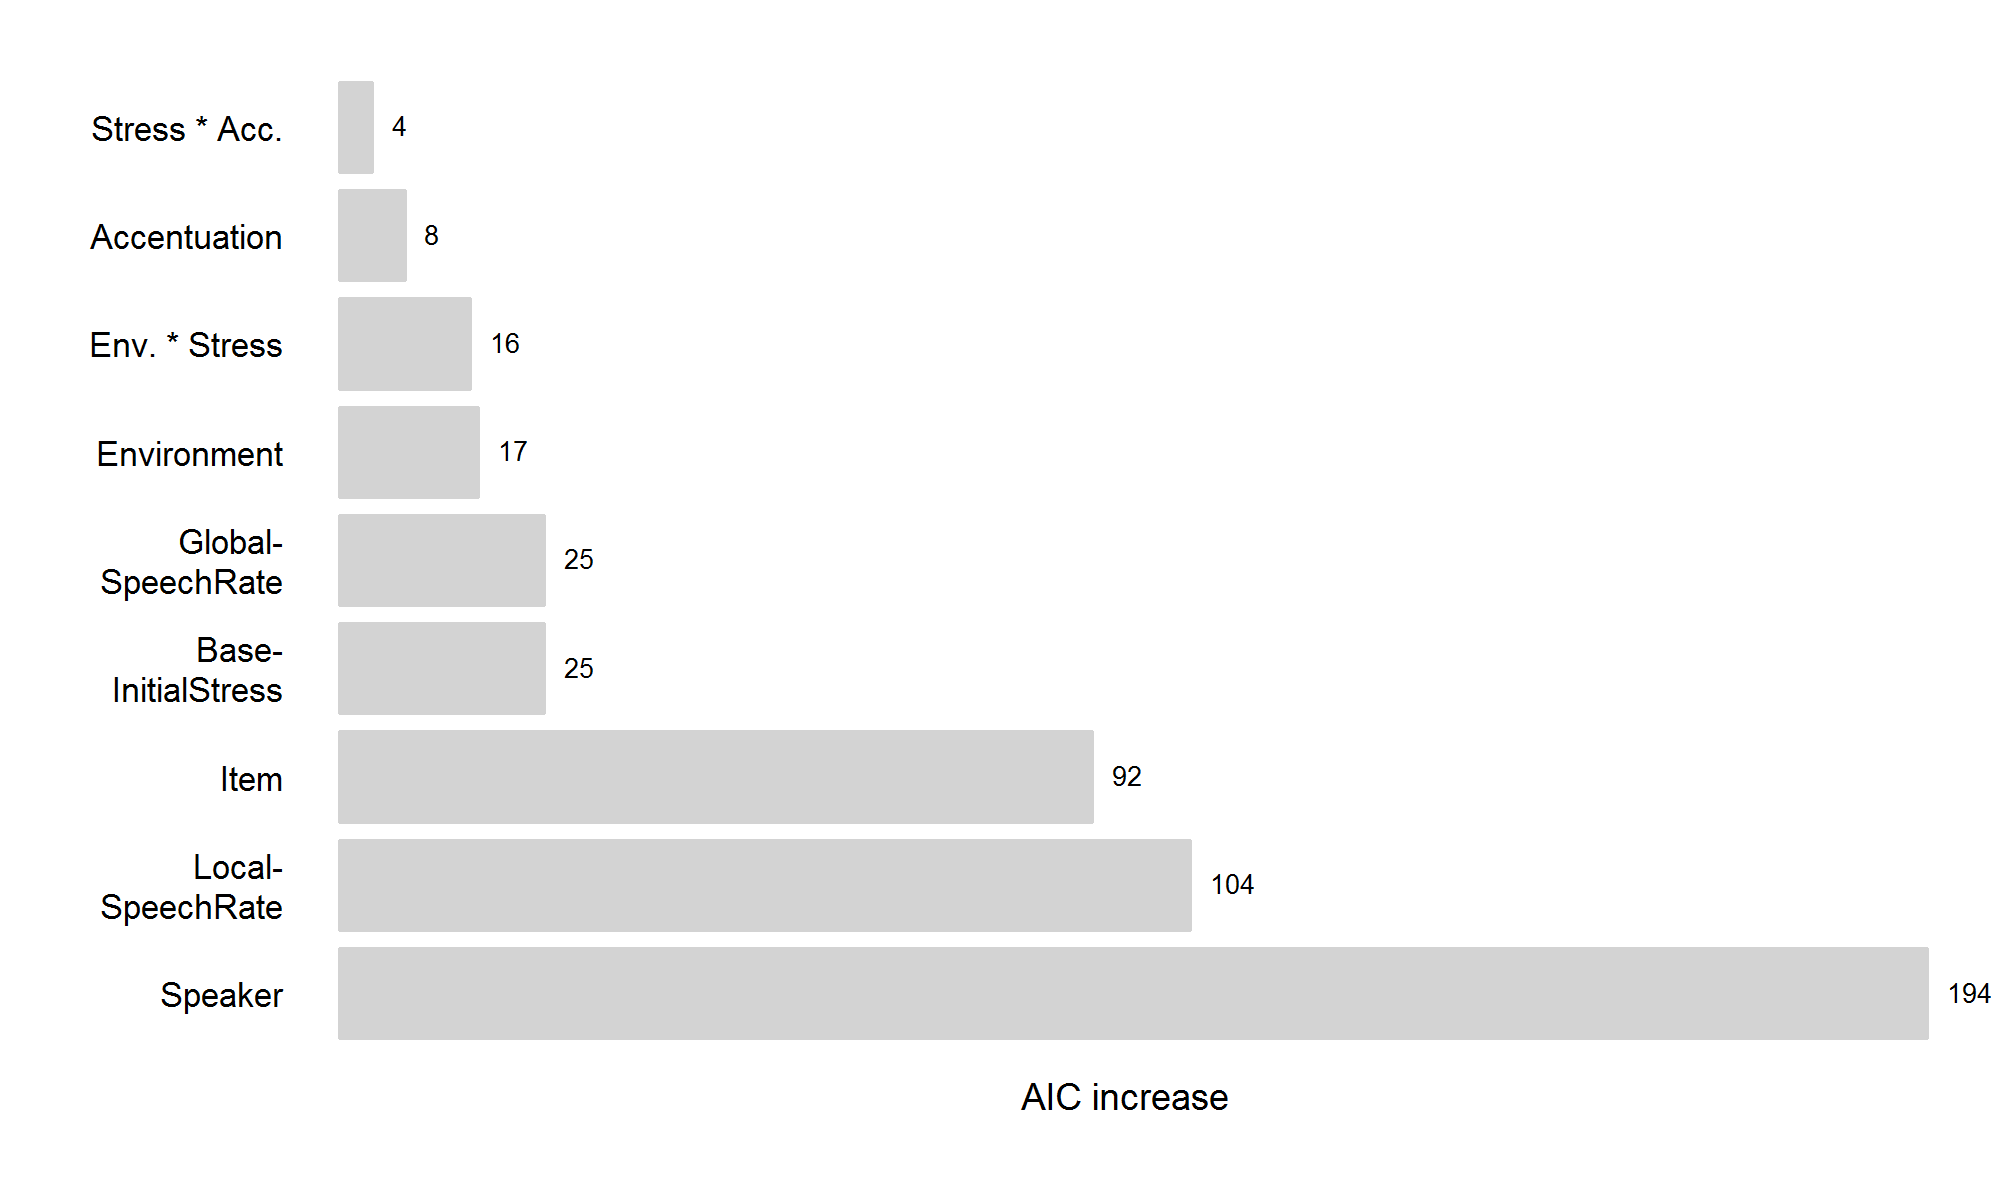
\includegraphics[scale=0.7]{images/Experiment/AICdecreaseImComplex.png}
	\caption{AIC increase for each variable of the final /ɪm/-model, AIC final model = \textminus6389}
	\label{fig:Effectsize im experiment}
\end{figure*}

% Ind. Contribution
To test the relative importance of each term in the final model, I looked at each term's contribution to the AIC of the final model. \figref{fig:Effectsize im experiment} displays the increase of the model's AIC  without each term. 
The figure shows that the noise variables \textsc{Speaker}, \textsc{LocalSpeechRate} and \textsc{Item} explain  most of the variation found in the data. They are followed by the two noise variables \textsc{GlobalSpeechRate} and \textsc{BaseInitialStress}. The variable of interest \textsc{Environment} explains much less of the variance found in the data. The analysis of the AIC increase thus shows that most of the variation in the data is explained by noise variables, i.e. not by the variable \textsc{Environment}. This supports the idea that \isi{gemination} with \is{im-}/ɪm/  is weaker in the experimental study than in the corpus study, and that, as proposed in the previous section, \isi{gemination} with the prefix \is{in-}\prefix{in} is weaker than \isi{gemination} with the prefix  \is{un-}\prefix{un}. 




% PC
None of the \is{decomposability measure}decomposability measures showed a significant effect in the final model when tested individually. To test possible effects of a combined \isi{decomposability} measure, an additional mixed model with combined \is{decomposability measure}decomposability measures was fitted to the data set.  
To attain these combined \is{decomposability measure}decomposability measures, I fitted a principal components analysis to the scaled variables scaled\textsc{Affix}, scaled\textsc{RelativeFrequency}, scaled\textsc{SemanticTransparencyRating}, scaled\textsc{Type-OfBase} and scaled\textsc{SemanticTransparency}.





\tabref{tbl: summary PC im exp} summarizes the principal components analysis. In the upper part of the table the loadings of each \is{principal component analysis}principal component are shown. The lower part of the table displays the proportion of variance accounted for by each component. 
Most of the variance is explained by the first \is{principal component analysis}principal component. The second, third and fourth component explain much less of the variance and the fifth hardly any.  The first four components were tested in the model. 


\begin{table}[b]
	\caption{Summary of principal components}
	\label{tbl: summary PC im exp}
	\resizebox{\textwidth}{!}{%		
		\begin{tabular}{l *{5}{S[table-format=+1.3]}}
			\lsptoprule
			 &  {PC1} &   {PC2} &  {PC3} & {PC4} & {PC5}  \\
			\midrule
			\multicolumn{6}{l}{Composition of principal components}\\\midrule
			scaled\textsc{Affix } & 0.437 & -0.407 & 0.154 & -0.785 & 0.056 \\ 
			scaled\textsc{RelativeFrequency }  & 0.314 & 0.808 & 0.407 & -0.147 & 0.247 \\ 
			scaled\textsc{SemanticTransparencyRating}  & 0.431 & 0.275 & -0.851 & -0.076 & -0.090 \\ 
			scaled\textsc{TypeOfBase }& 0.526 & -0.070 & 0.291 & 0.335 & -0.722 \\ 
			scaled\textsc{SemanticTransparency } & 0.497 & -0.317 & 0.038 & 0.494 & 0.637 \\ 			
			\midrule
			\multicolumn{6}{l}{Variance explained by principal components}\\
			\midrule
			Proportion of Variance &0.542 & 0.185 & 0.117 & 0.102 & 0.054\\
			\lspbottomrule
		\end{tabular}} 
\end{table}



This first component is composed of all five measures. This can be as seen by its loadings which are roughly the same for all variables. The second component is dominated by the variables scaled\textsc{RelativeFrequency} and scaled\textsc{Affix}, the third by scaled\textsc{SemanticTransparencyRating} and the fourth by scaled\textsc{Affix}, scaled\textsc{TypeOfBase} and scaled\textsc{SemanticTransparency}. 


The model with the principal components was fitted similarly to the model with the individual \is{decomposability measure}decomposability measures. After I simplified the model, it turned out that all terms which are significant in the final model with the individual \is{decomposability measure}decomposability measures are also significant in the final model with the principal components. On top of the effects significant in the model with the individual measures, the \is{principal component analysis}{principal component model} shows an effect of the fourth \is{principal component analysis}principal component (see \tabref{model im PC Experiment} in \hyperref[Appendix H: Model Summaries Experiment]{Appendix H} for a summary of the final model). \figref{fig:PC 4 imComplex experiment} shows the effect of \textsc{PC4}.

\begin{figure*} 
	

	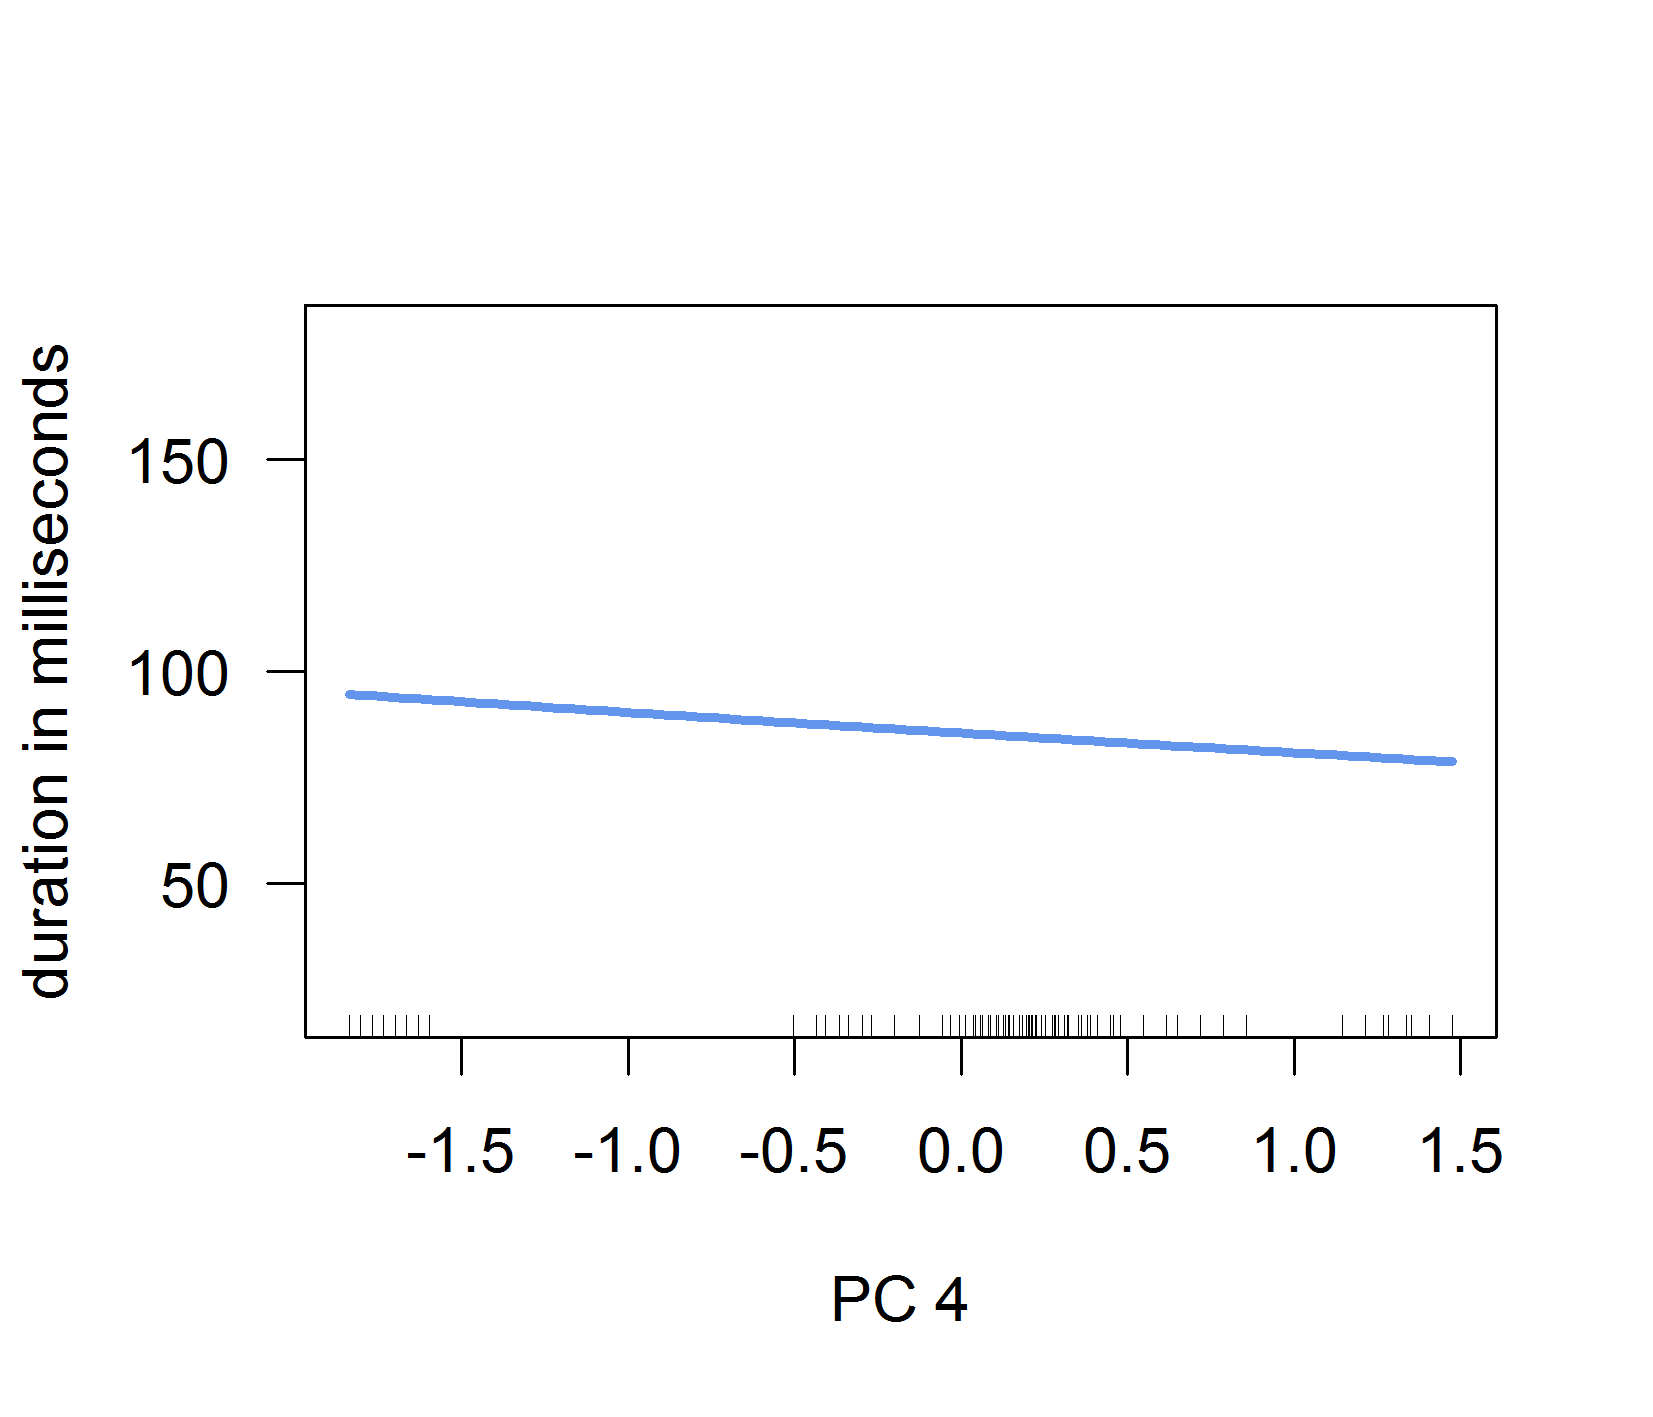
\includegraphics [scale=0.5] {images/Experiment/imModelPC}
	\caption{Effect of PC4 on consonant duration in complex /ɪm/-data set}
	\label{fig:PC 4 imComplex experiment}

\end{figure*}


The figure shows that with an increasing \textsc{PC4}-value, the nasal in /ɪn/-prefixed words becomes shorter. The size of the effect is, however, rather small. 
As described above, \textsc{PC4} is mostly composed of the variables \textsc{Affix}, \textsc{SemanticTransparency} and \textsc{TypeOfBase}. As indicated by the loadings shown in \tabref{tbl: summary PC im exp}, the component negatively correlates with \textsc{Affix}, meaning that a higher \textsc{PC4}-value represents \is{negative in-}negative \prefix{in}, and a lower value represents \is{locative in-}locative \prefix{in}. For \textsc{Semantic- Transparency} and \textsc{TypeOfBase}, the component shows positive loadings. This means that a higher \textsc{PC4}-value represents opaque derivatives with a bound base, and that a lower \textsc{PC4}-value represents transparent derivatives with words as bases.
The effect of \textsc{PC4} on nasal duration can thus be interpreted as follows: nasals in opaque \is{negative in-}negative \prefix{in}prefixed words with a bound base tend to be shorter than nasals in transparent \is{locative in-}locative \prefix{in}prefixed words with words as bases. This interpretation is supported by the fact that all tokens with a \textsc{PC4}-value lower than $-1.5$ are \is{locative in-}locative \prefix{in}prefixed words with a word as a base and transparent meaning (e.g. \textit{implant, imprison}). It is yet unclear why these words feature a particularly long nasal. 
It seems though that \textsc{PC4} reflects an effect on prefixal consonant duration that is restricted to a small number of types with a particular feature combination. This feature combination does not appear to directly translate to \isi{decomposability}.  
Instead, it might be related to the existence of two different \is{locative in-}locative \prefix{in}prefixes. 

As discussed in \sectref{locative in}, there might be two distinct \is{locative in-}locative \prefix{in}prefixes: native and non-native \is{locative in-}locative \prefix{in}. The two types of \is{locative in-}locative \prefix{in} are argued to differ in their origin, the type of base they take and their \isi{productivity}. The items with a low \textsc{PC4}-value seem to represent items with native \is{locative in-}locative \prefix{in}, i.e. \is{locative in-}locative \prefix{in}items with a transparent meaning and a native and free base. (e.g. \textit{implant}, \textit{imprison}). It remains unclear why they feature particularly long nasals.



To summarize,  doubles with the allomorph \is{im-}/ɪm/  are only longer than singletons in complex words when the base-initial syllable of the derivative is \is{stress}stressed. This is similar to what was found with the allomorph /ɪn/. The singleton-gemi-nate ratio for \is{im-}/ɪm/  in the experimental study is smaller than the one found in the corpus study, and also smaller than the one found for \is{un-}\prefix{un}. 
The model which tested combined \is{decomposability measure}decomposability measures furthermore shows a significant effect of one \is{principal component analysis}principal component on nasal duration with \is{im-}/ɪm/. However, the effect is relatively small and not clearly interpretable in terms of \isi{decomposability}. Crucially, the effect does not affect \isi{gemination}.




\subsubsection{The allomorph /ɪm/: Complete model}

The model predicting consonant duration with all \is{im-}/ɪm/-words ($N=1635$) was fitted according to the modeling procedure described in \sectref{stats}.  Because the initial model showed a non-normal distribution,  37 outliers (2.63\% of the data) were removed and the dependent variable was Box-Cox transformed ($\lambda = 0.343$). 
After the transformation, the model showed a satisfactory distribution of residuals. The model was then simplified and interactions were tested (see \hyperref[Appendix G Summaries of tested interactions in experimental study]{Appendix G} for a list of all tested interactions). 

 
The final model features the five variables \textsc{Environment}, \textsc{BaseInitialStress}, \textsc{PrePause}, \textsc{LocalSpeechRate} and \textsc{GlobalSpeechRate} (see \tabref{model im complete experiment} in \hyperref[Appendix H: Model Summaries Experiment]{Appen\-dix H} for a summary of the final model). Both \is{speech rate}speech rates show the expected effects. With increasing \is{speech rate}speech rates, the nasal becomes shorter. The three variables \textsc{Environment}, \textsc{BaseInitialStress}, and \textsc{Pause} form a three-way interaction. The interaction is shown in \figref{fig:NumNasal imCompleteexperiment}.

\begin{figure*}
	
	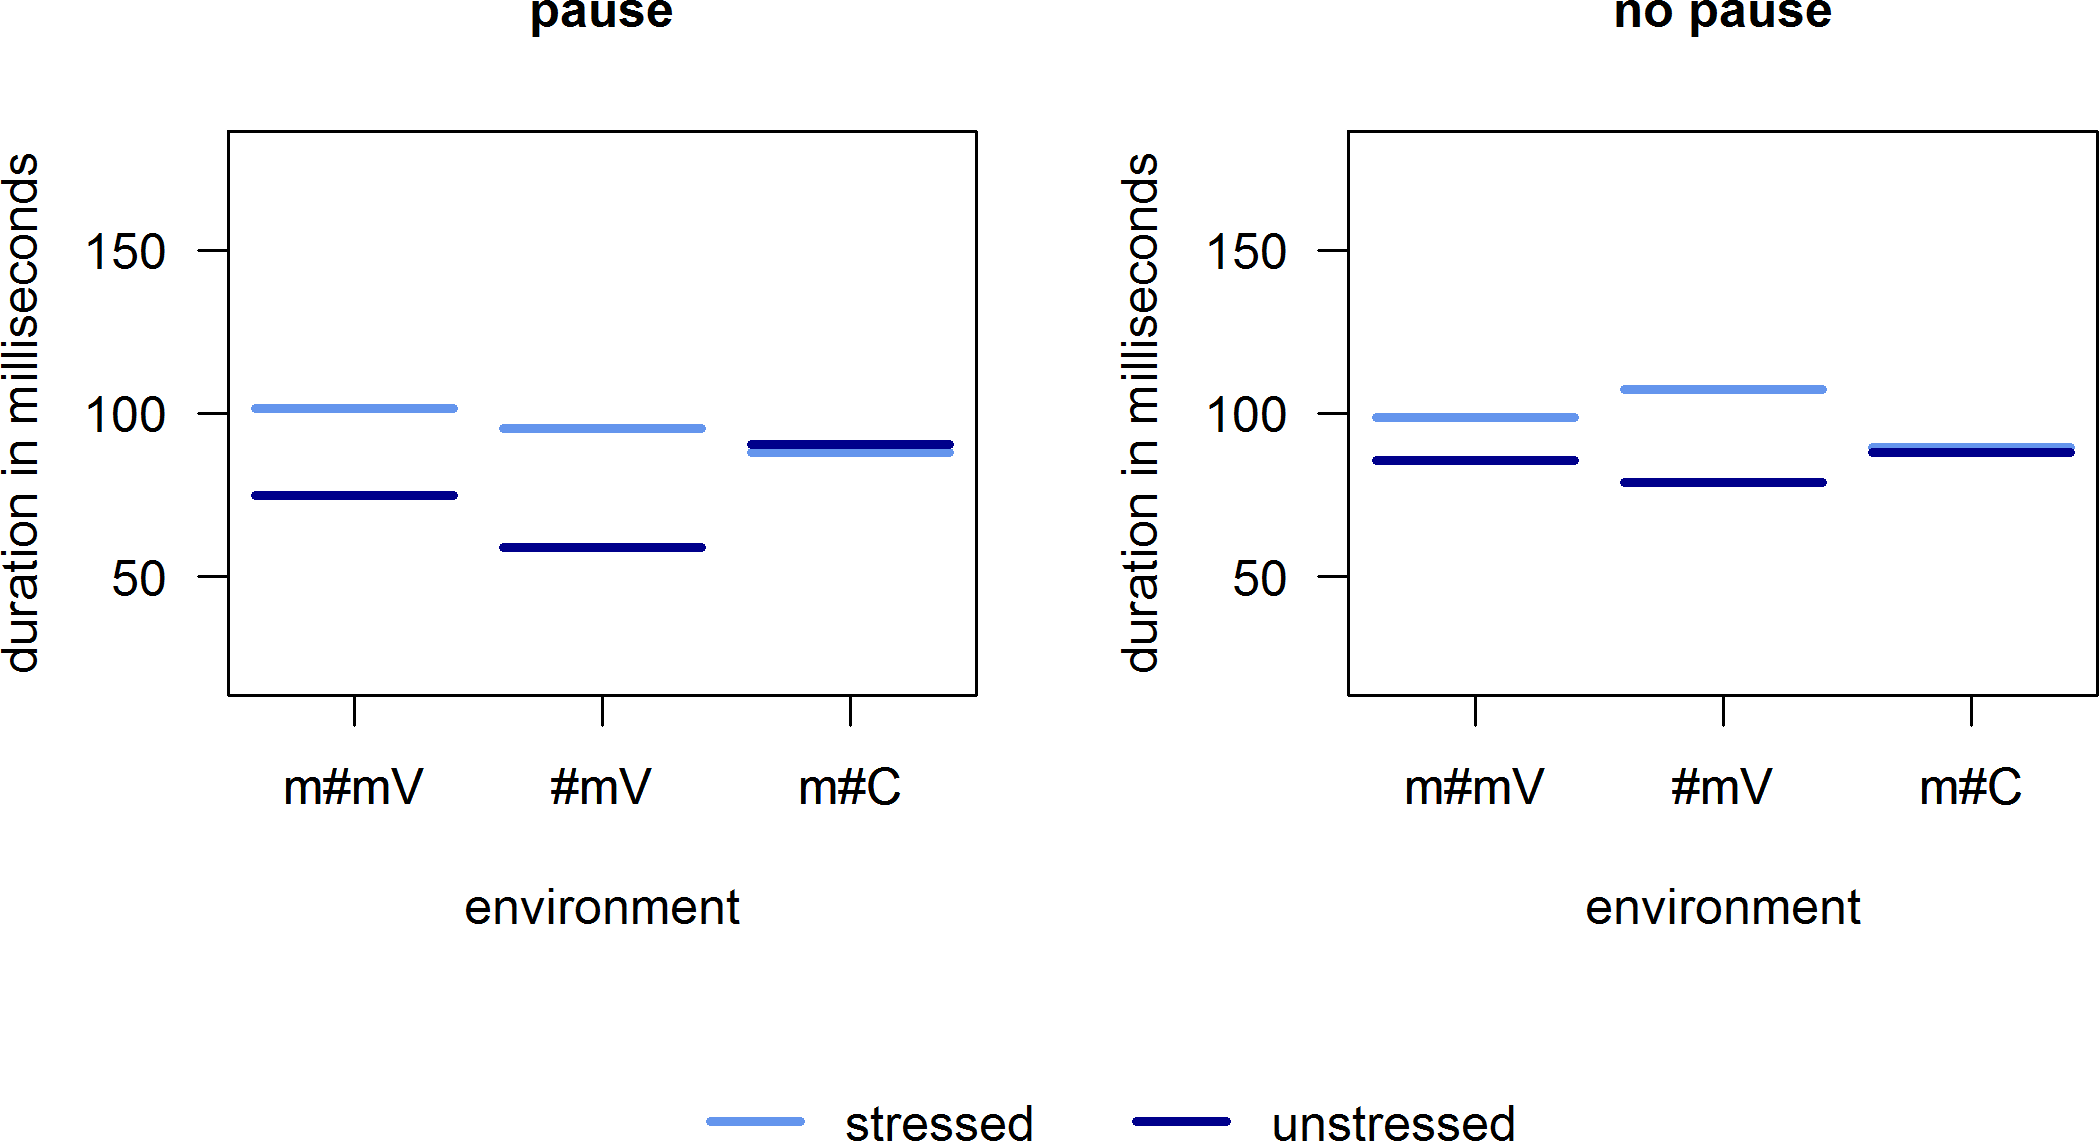
\includegraphics [scale=0.6] {images/Experiment/imModelCompleteInterEnvStressPause}
	
	\caption{Effect of base-initial stress by environment on consonant duration in /ɪm/-data set}
	\label{fig:NumNasal imCompleteexperiment}
\end{figure*}


The left panel of the figure shows the effect of \textsc{BaseInitialStress} by \textsc{Environment} for items produced with a pause before the item. The right panel shows the effect for items produced without a preceding pause. For each environment, light blue lines indicate the durations for items with a \is{stress}stressed base-initial syllable, and dark blue lines indicate the durations for items with an unstressed base-initial syllable.


In the left panel, i.e. in items with a preceding pause, doubles (\texttt{m\#mV}) are longer than singletons in base words (\texttt{\#mV}). This is independent of the \isi{stress} status of the base-initial syllable. Doubles are, however, only longer than singletons in complex words (\texttt{m\#C}) when the base-initial syllable is \is{stress}stressed.
In the right panel, i.e. in items without a preceding pause, doubles (\texttt{m\#mV}) are only longer than singletons in base words (\texttt{\#mV}) when the base-initial syllable is unstressed. In this case, they are as long as singletons in complex words (\texttt{m\#C}). For items with a \is{stress}stressed base-initial syllable, doubles (\texttt{m\#mV}) are shorter than singletons in base words (\texttt{\#mV}) but longer than singletons in complex words (\texttt{m\#C}).

To summarize, independent from a preceding pause, doubles in words with a \is{stress}stressed base-initial syllable are predicted to be longer than singletons in complex words. Depending on the absence or presence of a preceding pause, doubles in words with an unstressed base-initial syllable are either as long as or shorter than singletons in complex words. They are never predicted to be longer than singletons in complex words. 
Except for when the double consonant is part of a word which is not preceded by a pause and which features a \is{stress}stressed base-initial syllable, doubles are longer than singletons in base words with the same condition.


\subsubsection{Summary}\largerpage


In all \is{in-}\prefix{in}models, the noise variables behaved as expected. Decomposability does not seem to influence nasal duration with \is{in-}\prefix{in}. Only in one model, one \isi{decomposability} measure affected nasal duration (\textsc{PC4}). Its effect was very weak and not clearly interpretable in terms of \isi{decomposability}. It did not affect \isi{gemination}.


For both allomorphs of \is{in-}\prefix{in}, the analyses have shown that doubles are only longer than singletons when the base-initial syllable of the derivative is \is{stress}stressed. These doubles are, however, only longer than some types of singletons, and durational differences between doubles and singletons are often rather small. 
In case of /ɪn/, doubles in words with a \is{stress}stressed base-initial syllable are only longer than singletons in complex words with a following vowel. Doubles are not predicted to be longer than singletons in complex words with a following consonant or singletons in base words. 
For \is{im-}/ɪm/, doubles in words with a \is{stress}stressed base-initial syllable are longer than singletons with a following consonant but the durational difference between doubles and singletons is rather small.
Furthermore, doubles are slightly longer than singletons in base words.


The results suggest that \isi{gemination} with \is{in-}\prefix{in} depends on \isi{stress} and that the \isi{degree of gemination} with \is{in-}\prefix{in} is rather weak. Only when the base-initial syllable of a word is \is{stress}stressed, doubles are longer than some types of singletons, i.e. for /ɪn/, they are longer than singletons in complex words followed by a vowel, and for \is{im-}/ɪm/, they are longer than singletons in complex words followed by a consonant. Durational differences between doubles and singletons are rather small. This result is quite different from what was found for \is{un-}\prefix{un}. For \is{un-}\prefix{un}, doubles are longer than all types of singletons and the durational differences between doubles and singletons are much larger. One can thus state that the prefix \is{in-}\prefix{in} geminates, but that it geminates to a lesser degree than the prefix \is{un-}\prefix{un}.

Interestingly, the \isi{gemination} pattern found for \is{in-}\prefix{in} in the experimental study deviates from the one found in the corpus study. In the corpus study, \is{in-}\prefix{in} geminates independent of \isi{stress}, durational differences between doubles and singletons are bigger, and the \isi{degree of gemination} is the same as for \is{un-}\prefix{un}. In other words, \isi{gemination} with \is{in-}\prefix{in} is weaker in the experimental study than in the corpus study.

One possible explanation for the difference between corpus and experimental data is that the degree of \isi{semantic processing} differs between the two types of investigated speech. It can be hypothesized that in natural, \isi{conversational speech},  the \isi{semantic processing} of words is deeper than in \isi{read speech}, and that processing depth, in turn, affects \isi{gemination}. With deeper processing, the meaning of the affix is more present in the production of the derivative, leading to less \isi{reduction}, i.e. to \isi{gemination}. 
 In the corpus study, the meaning of the prefix is deeply processed, and it therefore clearly geminates. In the experimental study, in contrast, the affix's meaning is not processed deeply. In turn, \isi{gemination} is weaker and governed by a non-semantic factor,  i.e. the prosodic factor \isi{stress}.
  This explanation is supported by the fact that the variable \textsc{Affix} (\is{locative in-}locative \prefix{in} vs. \is{negative in-}negative \prefix{in}) only affects consonant duration with \is{in-}\prefix{in} in the corpus study, not in the experimental study. The meaning of the affix only affects consonant duration in the corpus data, where it is semantically processed. It does not affect consonant duration in the experimental data, where no deep \isi{semantic processing} takes place.





\subsection{The prefixes \prefix{un} and \prefix{in}}
The model predicting consonant duration with all complex \is{un-}\prefix{un} and /ɪn/-words ($N=3237$) was fitted to directly compare \isi{gemination} with \is{un-}\prefix{un} and \is{in-}\prefix{in}, and to further investigate the observed differences between the affixes.
As already discussed in \sectref{corpus un in}, in a model which investigates both prefixes, the \is{decomposability measure}decomposability variables cannot be tested in an interesting way. This is because \is{un-}\prefix{un}, as described in Sections~\ref{The decomposability of the four affixes: a comparison} and~\ref{decomposability experiment}, does not vary in most of the \is{decomposability measure}decomposability measures, and because \isi{relative frequency} measures are not well comparable across \is{un-}\prefix{un} and \is{in-}\prefix{in}. The prefix \is{in-}\prefix{in} has very many bound roots, which is problematic with regard to computing \isi{relative frequency} measures that are comparable to the \isi{relative frequency} measures of affixes with hardly any or no bound roots, i.e. in this case \is{un-}\prefix{un}. Therefore, none of the \is{decomposability measure}decomposability measures was tested in the model. 

 The model was fitted according to the modeling procedure described in \sectref{stats}. Due to an uneven distribution of the residuals in the initial model, the dependent variable \textsc{AbsoluteConsonantDuration} was Box-Cox-transformed ($\lambda = 0.061$) and 67 outliers were removed (2.07\% of the data).
The model was then simplified and interactions were tested (see \hyperref[Appendix G Summaries of tested interactions in experimental study]{Appendix G} for a list of all tested interactions).


The final model features the five variables \textsc{Environment}, \textsc{Affix}, \textsc{PrePause}, \textsc{Accentuation} and \textsc{LocalSpeechRate}. The variable \textsc{LocalSpeechRate} has the expected effect. The three variables \textsc{Environment}, \textsc{Affix} and \textsc{PrePause} interact. Furthermore, there is an interaction between \textsc{Environment} and \textsc{Accentuation}. The final model is summarized in \tabref{model in un experiment} in \hyperref[Appendix H: Model Summaries Experiment]{Appendix H}.


\figref{fig: Un In experiment Env and accent} shows the interaction between \textsc{Environment} and \textsc{Accentuation}. Estimates for \is{accentuation}accented items are shown in light blue, and estimates  for unaccented items are shown in dark blue. The figure shows that, independent of \isi{accentuation}, doubles (\texttt{n\#nV}) are clearly longer than singletons (\texttt{n\#C}, \texttt{n\#V}). In \is{accentuation}accented position, doubles are even longer. This has the effect that the durational difference between doubles and singletons increases in \is{accentuation}accented condition.



\begin{figure*}
	
	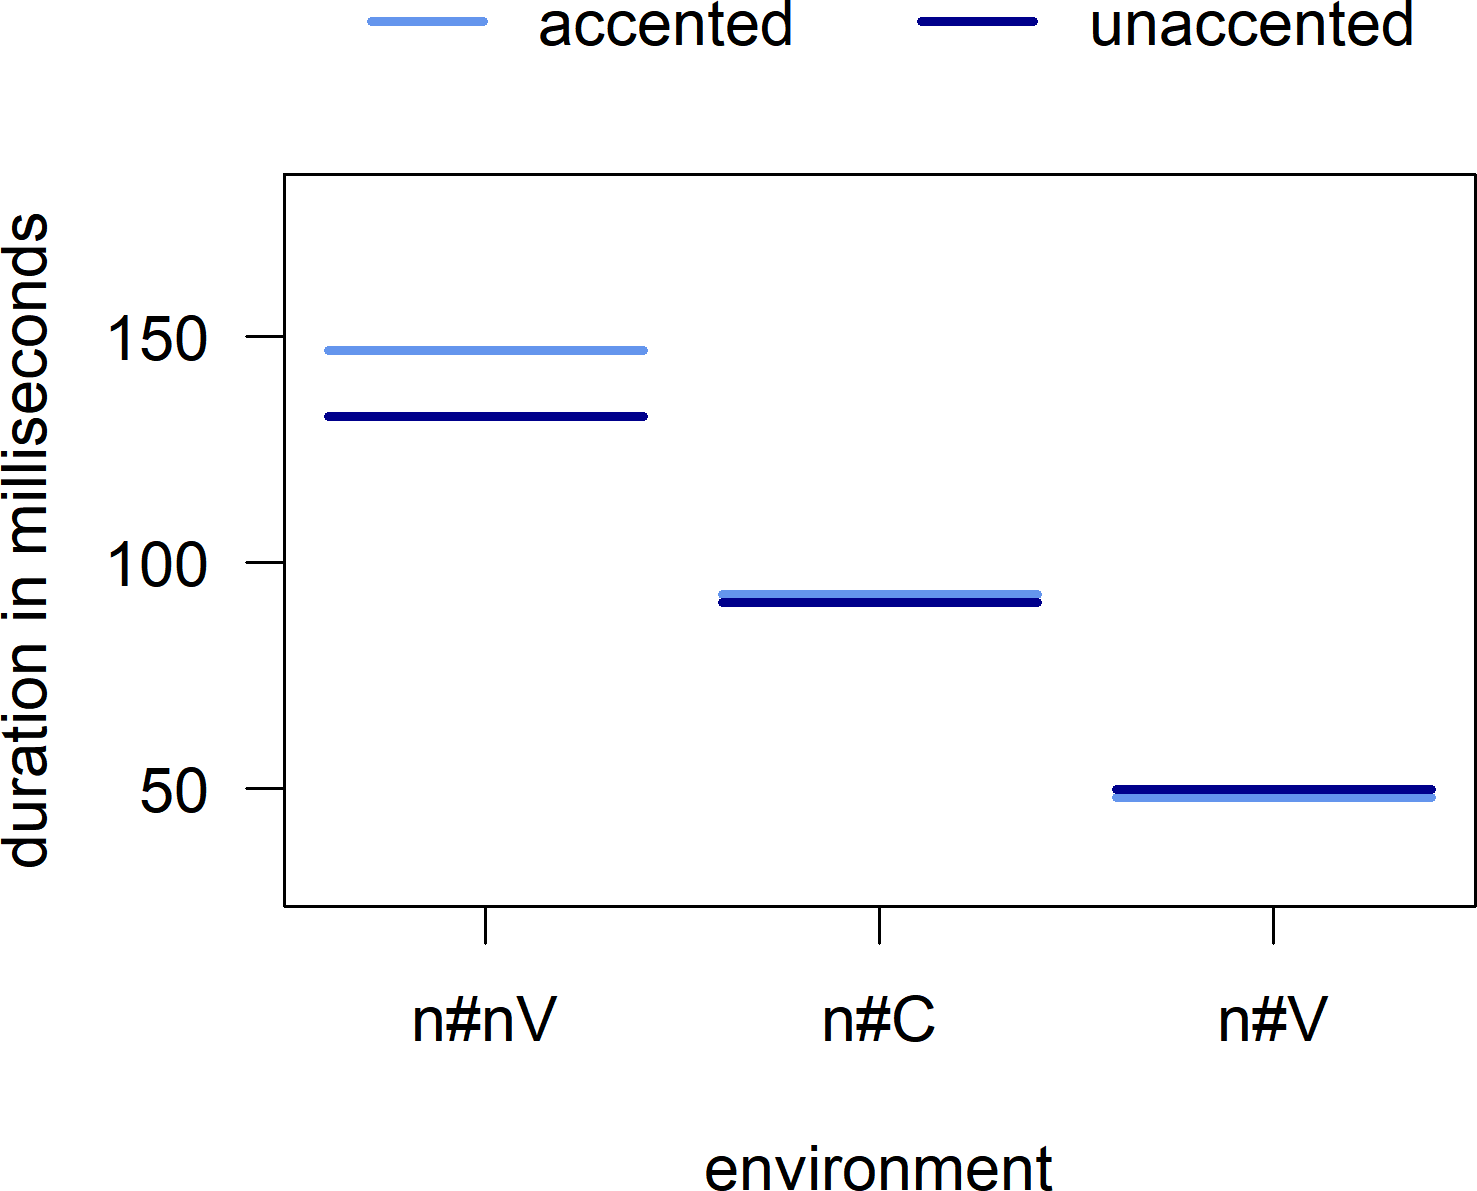
\includegraphics [scale=0.5] {images/Experiment/UnInInterEnvAcc}
	\caption{Effect of accentuation by environment on consonant duration in complex \prefix{un} and /ɪn/-words}
	\label{fig: Un In experiment Env and accent}
\end{figure*}

 However, to really interpret the \isi{gemination} pattern of the affixes, one must consider the three-way interaction between \textsc{Environment}, \textsc{Affix} and \textsc{PrePause}. The interaction is displayed in \figref{fig:Un In experiment}. In the left panel of the figure, the estimates for items with a preceding pause are shown. In the right panel of the figure, the estimates for items without a preceding pause are shown. For each affix, estimates for double consonants are shown in light blue, estimates for singletons followed by a consonant are shown in green, and estimates for singletons followed by a vowel are shown in dark blue.


\begin{figure*}[b]
	
	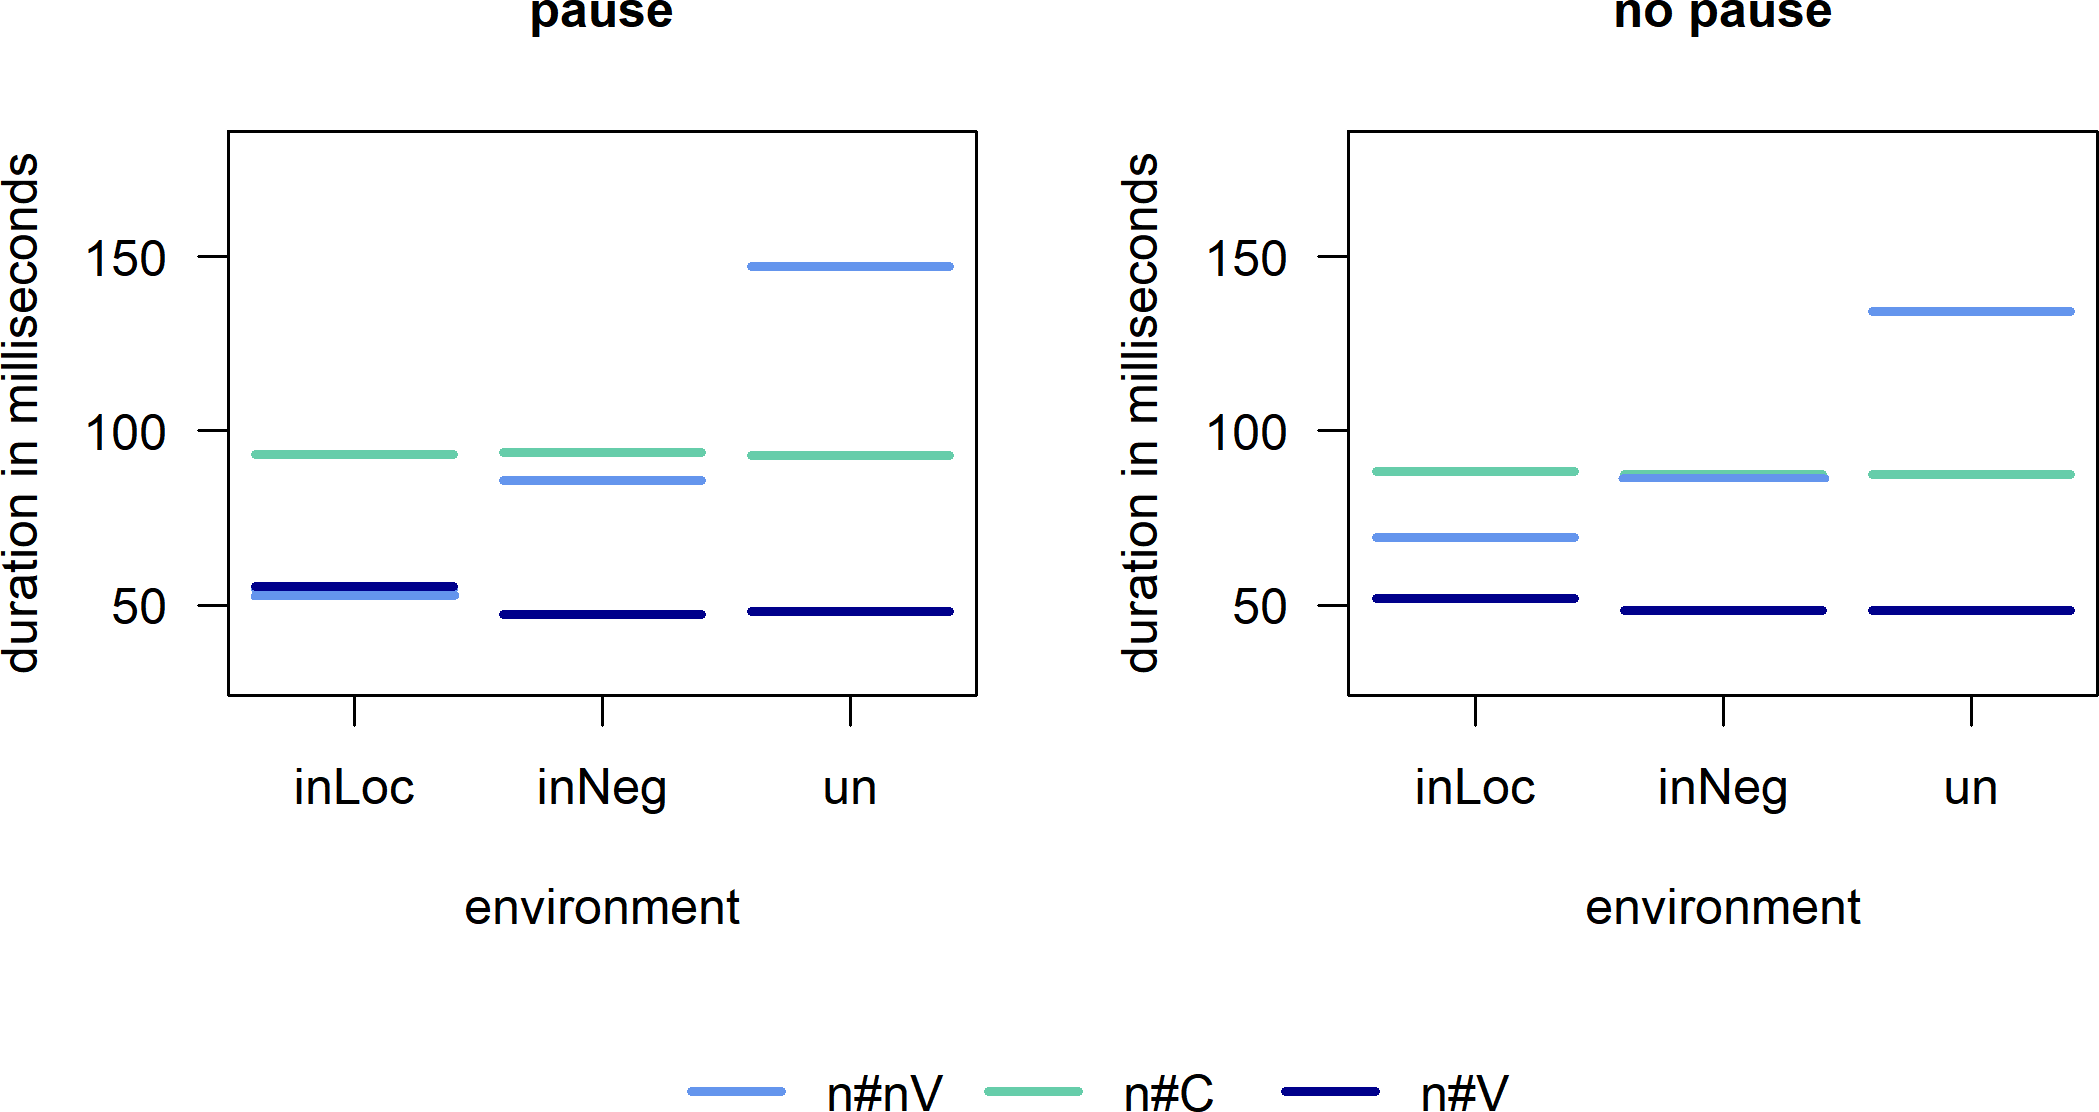
\includegraphics [scale=0.6] {images/Experiment/UnInInterEnvAffixPause1}
	
	\caption{Effect of environment by affix on consonant duration in complex \prefix{un} and /ɪn/-words with and without a preceding pause}
	\label{fig:Un In experiment}
\end{figure*}\pagebreak


In both panels of the figure, it is clearly visible that while the durations of the singletons do not differ much across affixes, the durations of the double consonants differ a lot across affixes. The double consonant in \is{un-}\prefix{un}prefixed words is much longer than the double consonant in both \is{in-}\prefix{in}prefixed words.
The double consonant in \is{negative in-}negative \prefix{in}prefixed words is longer than the one in \is{locative in-}locative \prefix{in}prefixed words. 
As a consequence, there are differences in \isi{gemination} between the affixes. 
 The prefix \is{un-}\prefix{un} clearly geminates, i.e. doubles are clearly longer than both singleton levels. 
For \is{negative in-}negative \prefix{in}, \isi{gemination} is weaker. Doubles are longer than singletons with a following vowel (\texttt{n\#V}), and about as long as singletons with a following consonant (\texttt{n\#C}). 
The double consonant in \is{locative in-}locative \prefix{in}words is the shortest. It is only longer than singletons which are followed by a vowel (\texttt{n\#V}) and preceded by a pause. It is debatable whether this difference between doubles and singletons with \is{locative in-}locative \prefix{in} can be interpreted as \isi{gemination} at all.

At first glance, the results suggest that the \isi{degree of gemination} decreases from \is{un-}\prefix{un} to \is{negative in-}negative \prefix{in}, to \is{locative in-}locative \prefix{in}.  However, one must be cautions with this interpretation. As already mentioned before, there are only four /ɪn/-prefixed types with a double consonant in the data set. Only one of these types features \is{locative in-}locative \prefix{in}, i.e. the conclusion that \is{locative in-}locative \prefix{in} geminates to a lesser degree than \is{negative in-}negative \prefix{in} is based on only one type. Furthermore, the type featuring \is{locative in-}locative \prefix{in} is the only type with an unstressed base-initial syllable in the data set. 
It might thus be the case that the difference between locative and \is{negative in-}negative \prefix{in} is actually caused by a difference in the prosodic structure of the words, i.e. by a difference in the \isi{stress} status of the base-initial syllable. There are two arguments for this explanation. First, the analysis of all \is{in-}\prefix{in}data has already shown that \isi{gemination} with \is{in-}\prefix{in} depends on the \isi{stress} status of the base-initial syllable. The effect of \isi{stress} was observed for both allomorphs of  \is{in-}\prefix{in}. Only when the base-initial syllable is \is{stress}stressed, \is{in-}\prefix{in} geminates. 
 Second, in none of the \is{in-}\prefix{in}analyses an effect of \textsc{Affix} was found. 


One can conclude that there is a difference in the \isi{degree of gemination} between \is{un-}\prefix{un} and the \is{in-}\prefix{in}prefixes: \isi{gemination} with \is{un-}\prefix{un} is stronger than \isi{gemination} with \is{in-}\prefix{in}. This might be explained with the fact that \is{un-}\prefix{un} is more segmentable and more informative than both \is{in-}\prefix{in}prefixes. However, there is no clear evidence for different degrees of \isi{gemination} between  \is{locative in-}locative \prefix{in} and \is{negative in-}negative \prefix{in}, even though the two \is{in-}\prefix{in}prefixes differ in \isi{segmentability} and \isi{informativeness}. Gemination with \is{in-}\prefix{in} depends on prosodic structure.

 This result is different from what was found in the corpus study. In the corpus study, \isi{gemination} was the same across \is{un-}\prefix{un} and \is{in-}\prefix{in} but there was a general durational difference between the affixes. The prefix \is{un-}\prefix{un} featured the longest nasal, followed by \is{negative in-}negative \prefix{in}. Locative \prefix{in} featured the shortest nasal. 
Even though the results differ, they can be interpreted similarly: the more segmentable the affix, or the more informative, the less \isi{reduction}. In the corpus study,  \isi{reduction} affected singletons and doubles. In the experimental study, only doubles were affected and there was no distinction between negative and \is{locative in-}locative \prefix{in}.






\subsection{The prefix \textit{dis-} }


\subsubsection{Complex model}

The model predicting consonant duration with all complex \is{dis-}\prefix{dis}words ($N=829$) was fitted according to the modeling procedure described in \sectref{stats}. Due to an uneven distribution of the residuals in the initial model, the dependent variable \textsc{AbsoluteConsonantDuration} was Box-Cox-transformed ($\lambda = 0.263$) and 16 outliers were removed (1.9\% of the data). After the model was refitted with the transformed dependent variable, it showed a satisfactory distribution of residuals. The model was then simplified and interactions were tested (see \hyperref[Appendix G Summaries of tested interactions in experimental study]{Appendix G} for a list of all tested interactions). The \is{decomposability measure}decomposability variables were tested individually.

The final model features three variables, \textsc{Environment}, \textsc{LocalSpeechRate} and \textsc{Accentuation}. The variable \textsc{LocalSpeechRate} behaves as expected: the higher the \isi{speech rate}, the shorter the consonant. The variables \textsc{Environment} and \textsc{Accentuation} form an interaction. The final model is summarized in \tabref{model dis complex experiment} in \hyperref[Appendix H: Model Summaries Experiment]{Appendix H}.

\begin{figure*}[b]
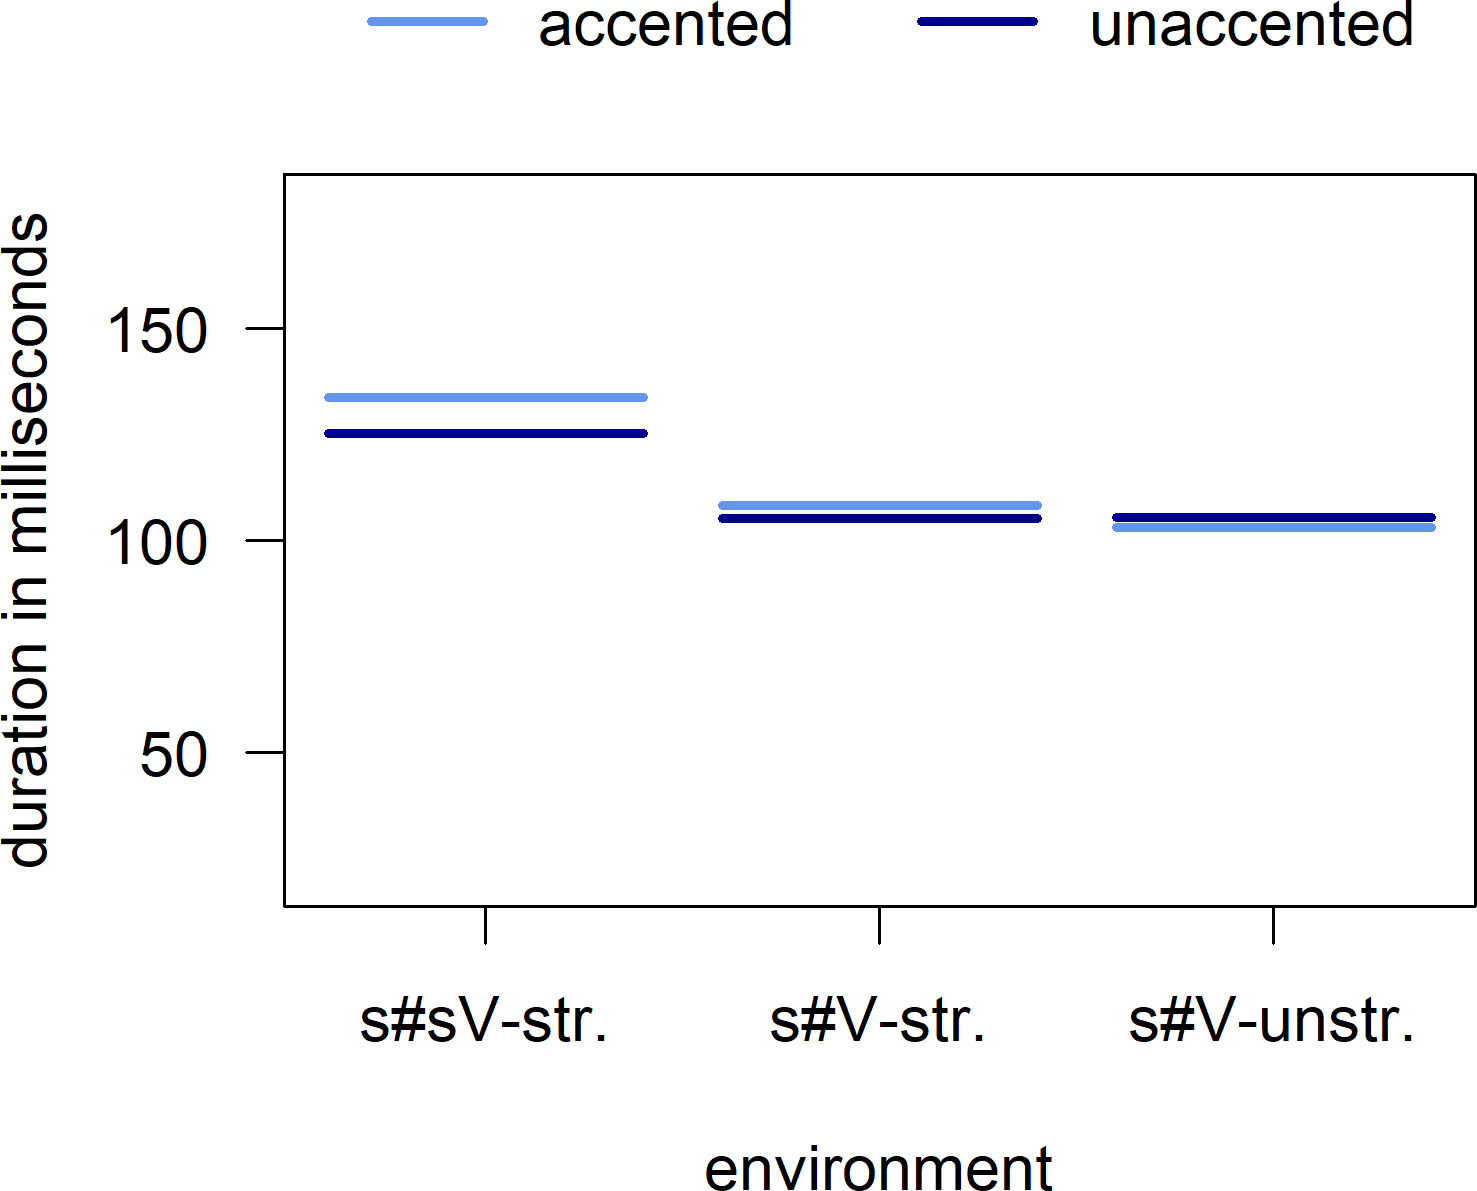
\includegraphics [scale=0.5] {images/Experiment/DisModelInterEnvAcc}
\caption{Effect of accentuation by environment on consonant duration in complex \prefix{dis}data set}
\label{fig:NumNasal disComplex experiment}
\end{figure*}\pagebreak

The interaction between \textsc{Environment} and \textsc{Accentuation} is depicted in \figref{fig:NumNasal disComplex experiment}. For each environment, the estimates for \is{accentuation}accented items are shown by light blue lines, and the estimates for unaccented items by dark blue lines.
The figure shows that,  
independent from \isi{accentuation}, doubles (\texttt{s\#sV-str.}) are longer than both types of singletons in complex words (\texttt{s\#V-str.}, \texttt{s\#V-unstr.}). The durational differences between doubles and singletons are larger in the \is{accentuation}accented than in the unaccented condition. 
In \is{accentuation}accented condition, doubles are 25\,ms longer than singletons with a \is{stress}stressed base-initial syllable and 30\,ms longer than singletons with an unstressed base-initial syllable. 
In unaccented condition, doubles are 20\,ms longer than both types of singletons. 
The durational difference between the two singleton levels is not significant.

As doubles are longer than both types of singletons, one can state that \is{dis-}\prefix{dis} geminates. The durational differences between doubles and singletons are smaller than the ones found for \is{un-}\prefix{un}. They are in approximately the same range as the ones for /ɪn/. This suggests that \is{dis-}\prefix{dis} geminates to a similar degree as \is{in-}\prefix{in}.



\figref{fig:Effectsize dis experiment} shows the contribution of each variable to the final model's goodness of fit.
The figure clearly shows that the variable \textsc{Speaker} explains most of the variance found in the data. The variable 
\textsc{Environment}, i.e. the crucial variable with regard to \isi{gemination}, explains much less of the variance. This fits in well with the interpretation that the prefix \is{dis-}\prefix{dis} geminates, but that it does not geminate to a high degree.


\begin{figure*}
	
	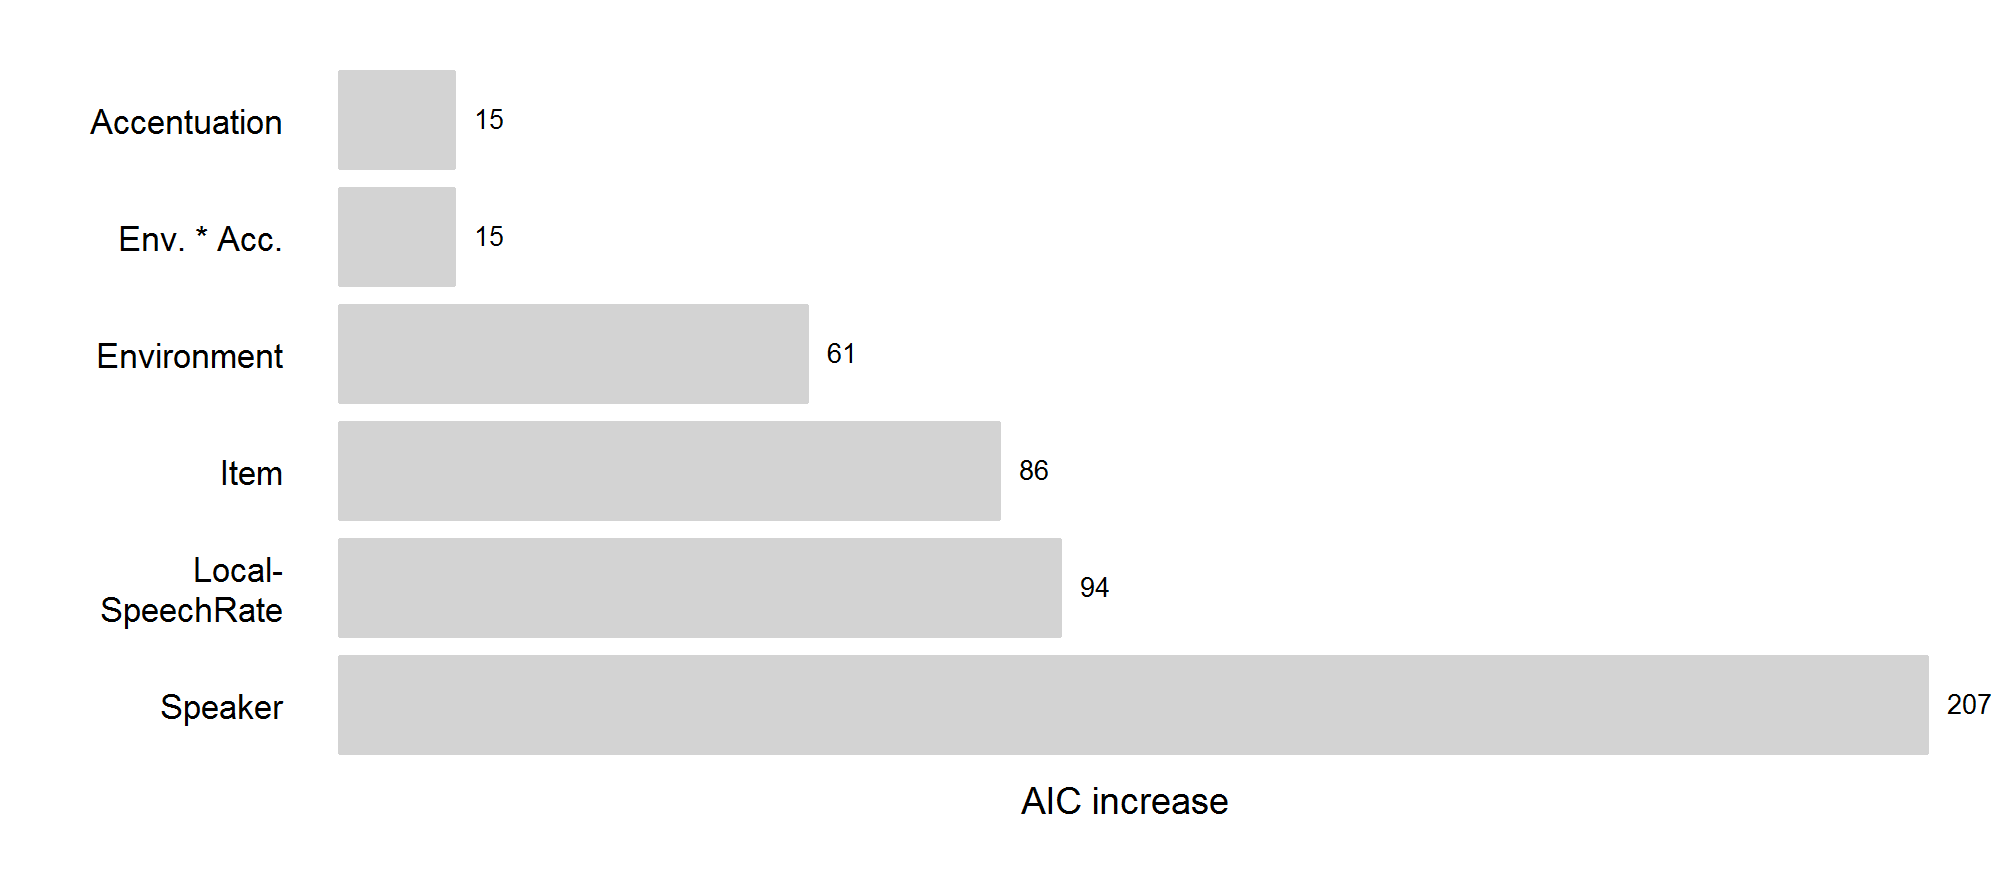
\includegraphics[scale=0.7]{images/Experiment/AICdecreaseDisComplex.png}
	\caption{AIC increase for each variable of the final \prefix{dis}model, AIC final model = \textminus4031}
	\label{fig:Effectsize dis experiment}

\end{figure*}



None of the individual \is{decomposability measure}decomposability variables proved to be significant in the final complex \is{dis-}\prefix{dis}model. To check whether a combined \isi{decomposability} measure affects consonant duration with \is{dis-}\prefix{dis}, I conducted a \is{principal component analysis}principal component analysis and tested the effect of the principal components in an additional model. The \is{principal component analysis}principal component analysis included the four variables log\textsc{RelativeFre-quency}, \textsc{SemanticTransparencyRating}, \textsc{TypeOfBase} and \textsc{SemanticTranspa-rency}. Categorical variables were recoded as numerical, and all variables were scaled. \tabref{tbl: summary PC dis exp} summarizes the principal components.



\begin{table*}
	\caption{Summary of principal components\label{tbl: summary PC dis exp}}
		\begin{tabular}{l *{4}{S[table-format=+1.3]}}
			\lsptoprule
			 &  {PC1} &   {PC2} &  {PC3} & {PC4}   \\
			\midrule
			\multicolumn{5}{l}{Composition of principal components}\\
			\midrule
			scaled\textsc{RelativeFrequency }  & -0.465& 0.817&0.344&0.005\\ 
			scaled\textsc{SemanticTransparencyRating}  &-0.489 &-0.559&  0.670 & 0.002 \\ 
			scaled\textsc{TypeOfBase }&-0.523& -0.098& -0.462& -0.710 \\ 
			scaled\textsc{SemanticTransparency } &-0.522& -0.104&-0.469&0.705 \\ 		
			\midrule
			\multicolumn{5}{l}{Variance explained by principal components}\\
			\midrule
			Proportion of Variance &0.644 &0.148 &0.112& 0.097\\
			\lspbottomrule			
		\end{tabular}
\end{table*}


Most of the variance is accounted for by the first component, the second and the third component explain much less variance, and the last \is{principal component analysis}principal component explains barely any variance. 
The first \is{principal component analysis}principal component is composed of all \is{decomposability measure}decomposability measures. The second component is mainly dominated by log\textsc{RelativeFrequency}, the third component mostly represents \textsc{TypeOfBase}, \textsc{SemanticTransparencyRating} and \textsc{SemanticTransparency}, and the fourth is mostly composed of \textsc{TypeOfBase} and \textsc{SemanticTransparency}. The first three principal components were included in the model.


The model was fitted similarly to the model with the individual \is{decomposability measure}decomposability measures. After model simplification, none of the principal components remained in the model. This means, the simplification of the model resulted in the same final model as the simplification of the model with the individual \is{decomposability measure}decomposability measures. Decomposability does not affect consonant duration with \is{dis-}\prefix{dis}.


\subsubsection{Complete model}\largerpage

The model predicting consonant duration with all \is{dis-}\prefix{dis}words ($N=1114$) was fitted according to the modeling procedure described in \sectref{stats}. Due to an uneven distribution of the residuals in the initial model, the dependent variable \textsc{AbsoluteConsonantDuration} was Box-Cox-transformed ($\lambda = 0.343$) and 24 outliers were removed (2.15\% of the data). After the model was refitted with the transformed dependent variable, it showed a satisfactory distribution of residuals.  The model was then simplified and interactions were tested (see \hyperref[Appendix G Summaries of tested interactions in experimental study]{Appendix G} for a list of all tested interactions). 

The final model features four variables: \textsc{LocalSpeechRate}, \textsc{Environment},\linebreak\textsc{Accentuation} and \textsc{PrePause}. The two noise variables \textsc{PrePause} and \textsc{LocalSpeechRate} behave as expected. With increased \isi{speech rate}, the fricative becomes long-er, and the fricative is longer when a pause precedes the item.
 The two variables \textsc{Environment} and \textsc{Accentuation} interact. The final model is summarized in \tabref{model dis complete experiment} in \hyperref[Appendix H: Model Summaries Experiment]{Appendix H}.




\figref{fig:  dis experiment Env and accent} shows the interaction between \textsc{Environment} and \textsc{Accentuation}. For each environment, the estimates for \is{accentuation}accented items are indicated by light blue lines, and the estimates for unaccented items are indicated by dark blue lines.
The plot reveals that doubles are longer than singletons in complex words (\texttt{s\#V-unstr.}, \texttt{s\#V-str.}) and singletons in simplex words (\texttt{sV-unstr.}). In \is{accentuation}accented condition, the durational differences between doubles and these two types of singletons is larger than in unaccented condition. 
Independent from \isi{accentuation}, doubles are shorter than singletons in base words (\texttt{\#sV-str.}).


\begin{figure*}
	
	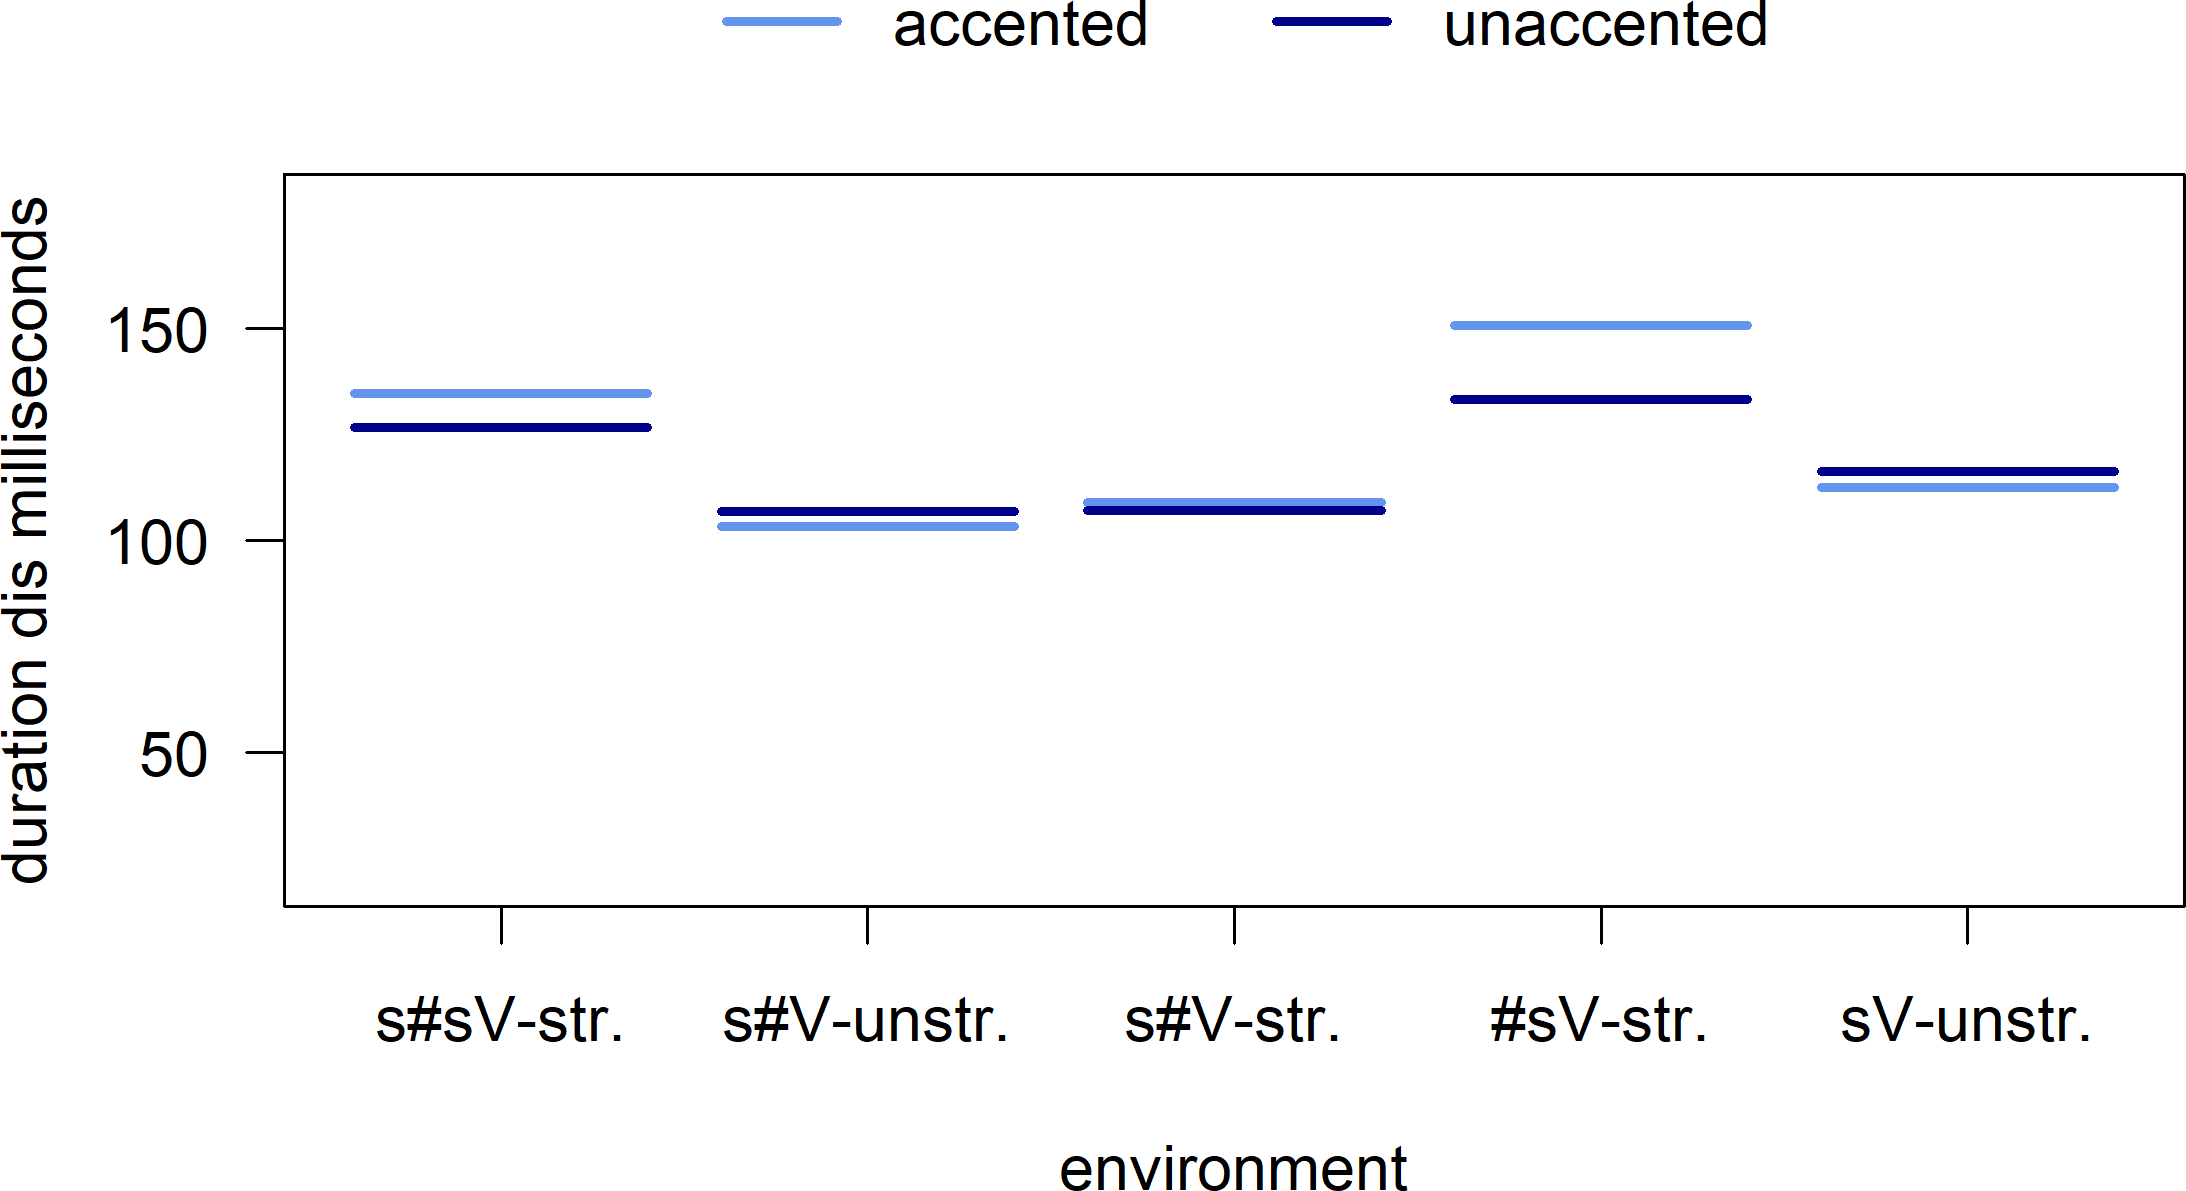
\includegraphics [scale=0.5] {images/Experiment/disModelCompleteinterEnvAcc}
	\caption{Effect of accentuation by environment on consonant duration in \prefix{dis}data set}
	\label{fig:  dis experiment Env and accent}
\end{figure*}


\hspace*{-0.27794pt}The figure, furthermore, indicates that singletons in simplex words (\texttt{sV-unstr.}) are not significantly longer than singletons in complex words (\texttt{s\#V-unstr.}, \texttt{s\#V- str.}). This, and the fact that they are shorter than phonological doubles, shows that \isi{gemination} with \is{dis-}\prefix{dis} is not an orthographic phenomenon but a morpho-phonological one. In other words, phonological doubles are longer than phonological singletons because of the presence of two underlying identical consonants, not because of the presence of two identical graphemes.



\subsubsection{Summary}

Both \is{dis-}\prefix{dis}models have shown the expected effects of the noise variables. With regard to the variables of interest, the complex model has revealed that \isi{decomposability} does not affect consonant duration with \is{dis-}\prefix{dis}. The variable \textsc{Environment} is significant in all models. Its effect shows that \is{dis-}\prefix{dis} geminates. The double in \is{dis-}\prefix{dis}prefixed words is longer than the singleton in complex words and the singleton in simplex words. 
In both models, there is an interaction between \textsc{Environment} and \textsc{Accentuation}, indicating that \isi{gemination} is stronger when the double consonant word is \is{accentuation}accented. This is similar to what was found for \is{un-}\prefix{un}.

That singletons in simplex words are shorter than phonological doubles shows that \isi{gemination} does not depend on \isi{orthography} but is a {morpho-phonological phenomenon}. If the lengthening of the phonological double was caused by its \isi{orthography}, i.e. by the fact that it is spelled with two graphemes, the singleton in simplex words, which is also represented by an orthographic double, should also be lengthened. This is not the case. 


The data suggests that the \isi{degree of gemination} with \is{dis-}\prefix{dis} is weaker than the \isi{degree of gemination} with \is{un-}\prefix{un}. Gemination with \is{dis-}\prefix{dis} seems to be similar in its degree to \isi{gemination} with \is{in-}\prefix{in}. 
This is indicated by the durational differences between doubles and singletons for \is{dis-}\prefix{dis}. They are smaller than the ones found for \is{un-}\prefix{un} and similar to the ones found for /ɪn/. 
Furthermore, in contrast to what was found for \is{un-}\prefix{un}, and similar to what was found for \is{in-}\prefix{in}, doubles with \is{dis-}\prefix{dis} are only longer than some types of corresponding singletons, i.e. doubles are not longer than singletons in base words.



A comparison of the durations of the experimental study with the ones of the corpus study reveals that \isi{gemination} with \is{dis-}\prefix{dis} is weaker in the experimental study than in the corpus study. Differences between doubles and singletons are larger in the corpus study than in the experimental study. The same pattern was observed for the prefix \is{in-}\prefix{in}.


\subsection{The suffix \textit{-ly} }

\subsubsection{Complex model}

The model predicting consonant duration with all complex \is{-ly}\suffix{ly}-words ($N=1205$) was fitted according to the modeling procedure described in \sectref{stats}. Due to an uneven distribution of the residuals in the initial model, the dependent variable \textsc{AbsoluteConsonantDuration} was Box-Cox-transformed ($\lambda = 0.263$) and 27 outliers were removed (2.24\% of the data). 
After the model was refitted with the transformed dependent variable, it showed a satisfactory distribution of residuals. The model was then simplified and interactions were tested (see \hyperref[Appendix G Summaries of tested interactions in experimental study]{Appendix G} for a list of all tested interactions). 

The final model features three variables of interest: \textsc{Environment}, log\textsc{Relat-iveFrequency} and \textsc{SemanticTransparencyRating}. It features five noise variables: \textsc{LocalSpeechRate}, \textsc{TypeOfL}, \textsc{PostPause}, \textsc{Accentuation} and \textsc{Preceding-SegmentDuration}. 
There are two interactions in the model, one between \textsc{Environment} and log\textsc{RelativeFrequency}, and one between \textsc{Environment} and \textsc{Accentuation}. 

Note that there is no suppression effect with the two \is{decomposability measure}decomposability variables in the model, i.e. the effects of  \textsc{SemanticTransparencyRating} and log\textsc{Rela\-tive\-Frequency} do not negatively affect each other in the model. Fitting the final model with only one of the two \is{decomposability measure}decomposability variables at a time, furthermore, revealed that their effect sizes do not change much in the presence of the other. Their effects are thus interpretable.
The final model is summarized in \tabref{model ly complex experiment} in \hyperref[Appendix H: Model Summaries Experiment]{Appendix H}.

The noise variables \textsc{LocalSpeechRate}, \textsc{TypeOfL}, \textsc{PostPause} and \textsc{Preceding- SegmentDuration} behave as expected. The higher the \isi{speech rate}, the shorter the lateral.; a tap /l/ is shorter than an approximant /l/; items which are followed by a pause feature a longer /l/ than items with no following pause; and with increased preceding segment duration, the duration of the lateral becomes shorter.


%Accentuation

The interaction between \textsc{Environment} and \textsc{Accentuation} is shown in \figref{fig:Env Acc lyComplex experiment}. 
For each environment, the estimates for \is{accentuation}accented items are shown by light blue lines, and the estimates for unaccented items are shown by dark blue lines. The estimated duration for singletons in complex words (\texttt{\#l-<l>}) is shown on the left, the estimated durations for the three double consonant environments \texttt{l\#l-<lel>}, \texttt{l\#l-<ll>} and \texttt{syll.l\#l-<ll>} are shown on the right. If \is{-ly}\suffix{ly} geminates, the estimated duration for the singleton should be shorter than the estimated durations for the three double environments. 


\begin{figure*}
	
	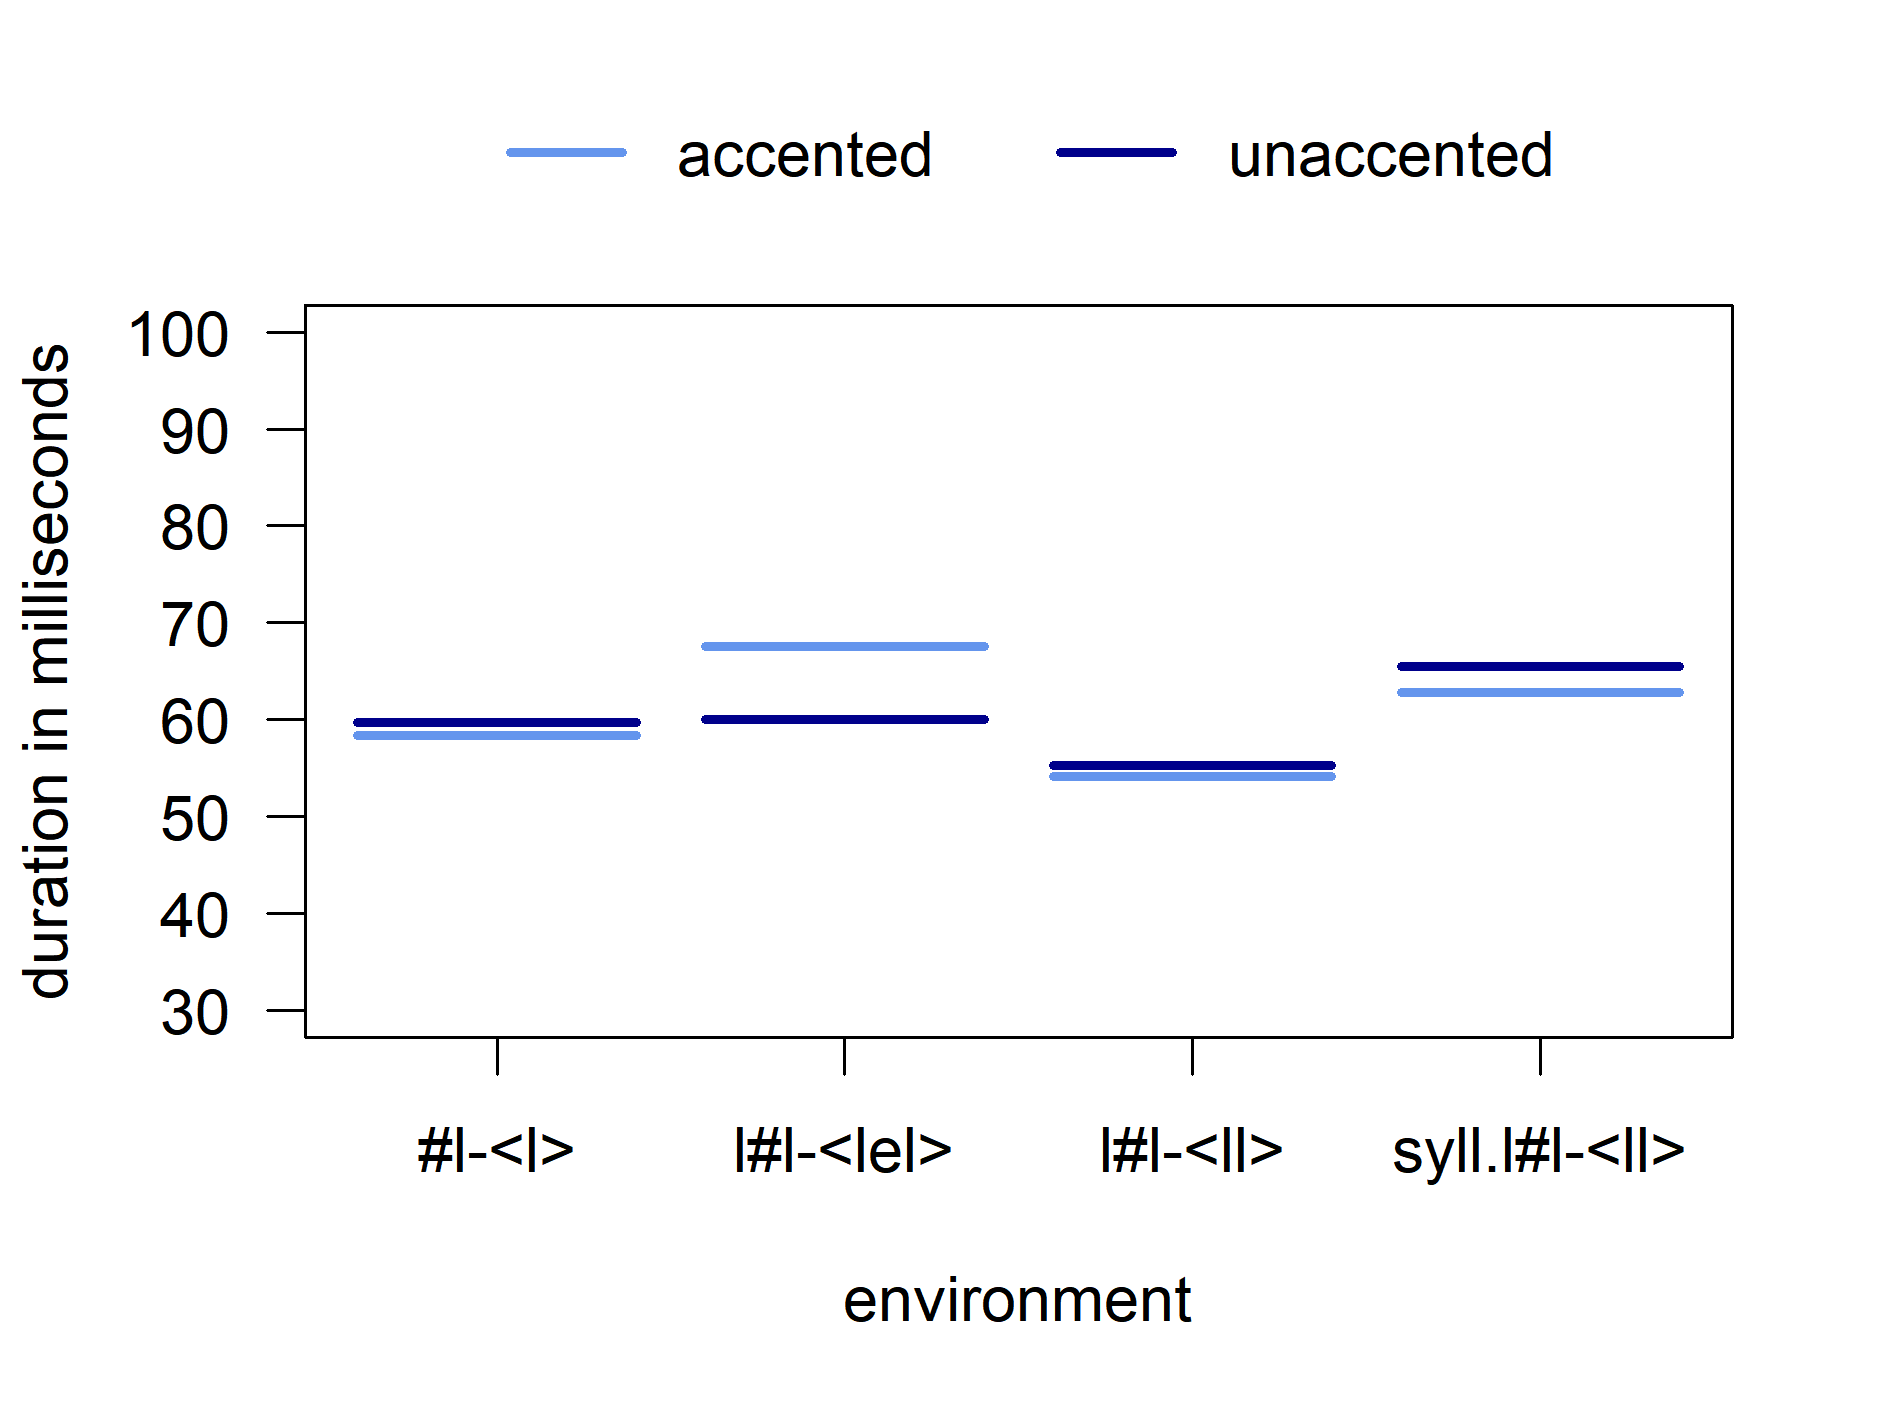
\includegraphics [scale=0.5] {images/Experiment/LyModelInterEnvAcc}
	\caption{Effect of accentuation by environment on consonant duration in complex \suffix{ly}-data set}
	\label{fig:Env Acc lyComplex experiment}
\end{figure*}

For items in \is{accentuation}accented position, doubles of the \texttt{l\#l-<ll>}-environment feature the shortest durations of all environments. This means that singletons (\texttt{\#l-<l>}) are estimated to have longer durations than this type of double consonant. This clearly speaks against \isi{gemination} with \is{-ly}\suffix{ly}. Doubles of the \texttt{l\#l-<lel>}-environ-ment feature the longest durations of all environments, and \is{syllabicity}syllabic doubles (\texttt{syll.l\#l-<ll>}) pattern in between singletons  (\texttt{\#l-<l>}) and doubles of the \texttt{l\#l- <lel>}- environment.


For items in unaccented position, doubles of the \texttt{l\#l-<ll>}-environment again feature the shortest durations, i.e. they are estimated to be shorter than the singletons in the data set. Syllabic doubles (\texttt{syll.l\#l-<ll>}) feature the longest lateral in this condition.  Singletons in complex words (\texttt{\#-<l>}) and doubles of the \texttt{l\#l-<lel>}- environment  pattern in between.

Crucially, in both conditions, i.e. \is{accentuation}accented and unaccented, singletons are not estimated to be shorter than all three types of double consonants. In fact, they are consistently estimated to be longer than doubles of the  \texttt{l\#l-<ll>}-environment. This speaks against \isi{gemination} with \is{-ly}\suffix{ly}.

One could, however, argue that the fact that doubles of the \texttt{l\#l-<lel>}- environment and doubles of the \texttt{syll.l\#l-<ll>}-environment are  longer than singletons speaks for \isi{gemination} with \is{-ly}\suffix{ly}. However, there is no evidence that these durational differences between doubles and singletons are caused by the presence of two underlying laterals. If that was the case, doubles of the \texttt{l\#l-<ll>}-environment would also be longer than singletons. 
Instead, the durational difference between singletons and doubles of the \texttt{l\#l-<lel>}-environment and doubles of the \texttt{syll. l\#l-<ll>} -environment can be attributed to the factors \isi{syllabicity} and \isi{orthography}. It can be assumed that doubles of the  \texttt{syll.l\#l-<ll>}-environment are longer than singletons because they are \is{syllabicity}syllabic, and that doubles of the  \texttt{l\#l-<lel>}-environment are longer because they are spelled with the orthographic sequence <lel>. 
 Overall, there is no evidence for \isi{gemination} with the suffix \is{-ly}\suffix{ly}.

% RelFreq

\begin{figure*}
	
	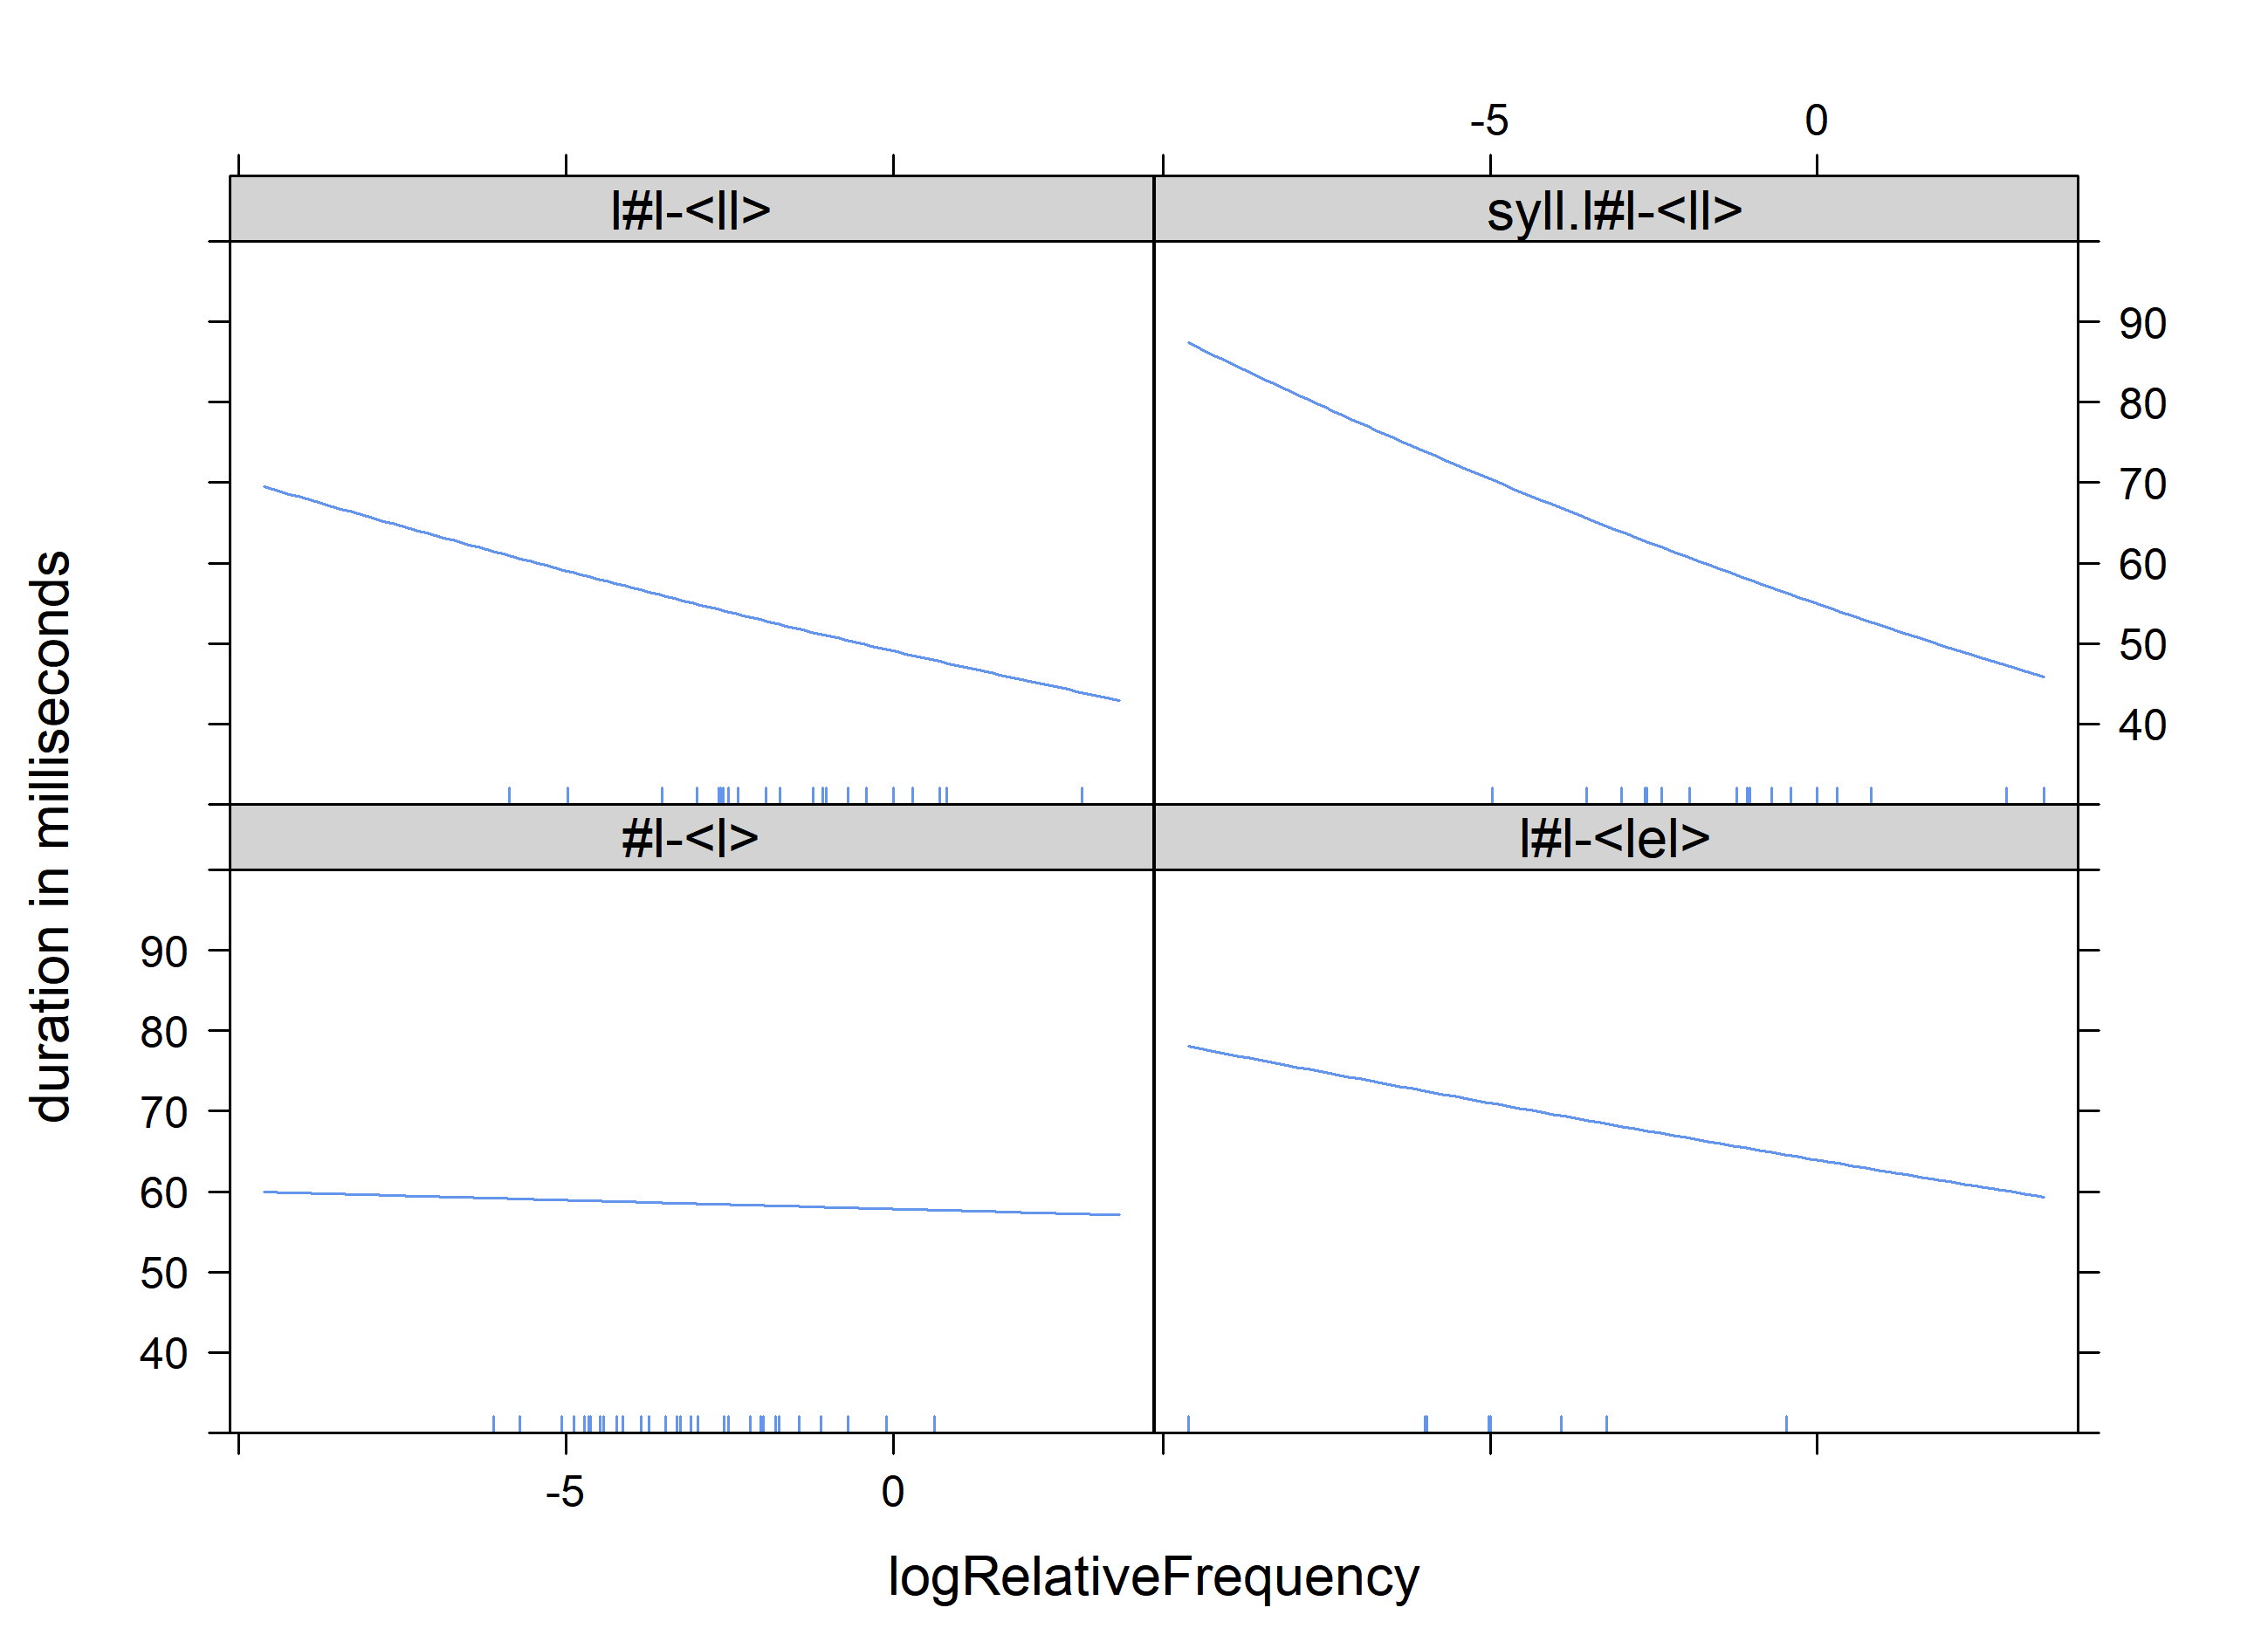
\includegraphics [scale=0.5] {images/Experiment/LyModelInterRelFreqEnv}
	\caption{Effect of relative frequency by environment on consonant duration in complex \prefix{ly}data set}
	\label{fig:Rel Env lyComplex experiment}
	
\end{figure*}



The variable \textsc{Environment} also forms an interaction with the variable log- \textsc{RelativeFrequency}. \figref{fig:Rel Env lyComplex experiment} shows the interaction. For each environment, the effect of \isi{relative frequency} is shown. 
The figure suggests that for the three double environments (\texttt{syll.l\#l- <ll>}, \texttt{l\#l-<ll>}, \texttt{l\#l-<lel>}), consonant duration decreases with increasing \isi{relative frequency}. The higher the \isi{relative frequency}, i.e. the less decomposable a word, the shorter the /l/. For the singleton environment, the predicted value does not change depending on \isi{relative frequency} (\texttt{\#l-<l>}).




However, it is very important to note that the effect of \isi{relative frequency} is only significant for \is{syllabicity}syllabic doubles (\texttt{syll.l\#l-<ll>}).  The effect is not significant for the other two double environments (\texttt{l\#l-<ll>}, \texttt{l\#l-<lel>}). 
Furthermore, it is unclear how trustworthy the effect for the \is{syllabicity}syllabic doubles really is. Looking at the rugs in the panel for the \is{syllabicity}syllabic doubles, it becomes obvious that for a large portion of the predicted \isi{frequency} range no observations exist. There is no item with a log\textsc{RelativeFrequency} below $-5$. 
Most types in the data set feature a log\textsc{RelativeFrequency} between $-5$ and $-0.9$, and there are only two types with a very high \isi{relative frequency}, i.e. a \isi{relative frequency}  above $2.5$. It can be assumed that the observed \isi{relative frequency} effect is caused by these two types (\textit{aerobically} and \textit{therapeutically}). 


To conclude, even though there seem to be tendencies for a \isi{relative frequency} effect on the duration of the two double environments  \texttt{l\#l-<ll>} and \texttt{l\#l-<lel>}, and even though there is a significant effect of \isi{relative frequency} for \is{syllabicity}syllabic doubles  (\texttt{syll.l\#l-<ll>}), the model does not provide convincing evidence for an effect of \isi{relative frequency} on the duration of phonological doubles.







%SemTrans
\figref{fig: Rating  lyComplex experiment} shows the effect of the \isi{decomposability} measure \textsc{SemanticTrans-parencyRating}. The figure shows that with a higher rating, i.e. with decreasing \isi{decomposability}, the lateral in \is{-ly}\suffix{ly}-suffixed words becomes shorter. This effect is expected. However, the size of the effect is quite small, i.e. durational differences are minimal.





To sum up, the complex model does not provide evidence for \isi{gemination} with \is{-ly}\suffix{ly}. Doubles are not systematically longer than singletons. 
The model shows two significant effects of \isi{decomposability}. Syllabic doubles with a low \isi{relative frequency} are predicted to be longer than \is{syllabicity}syllabic doubles with a high \isi{relative frequency}, and items which are rated as highly decomposable are predicted to feature a longer lateral than items which are rated as less decomposable. However, both effects are rather weak and the effect of \isi{relative frequency} might be caused by only a few types in the data set.



 

 
\begin{figure*}
	 
	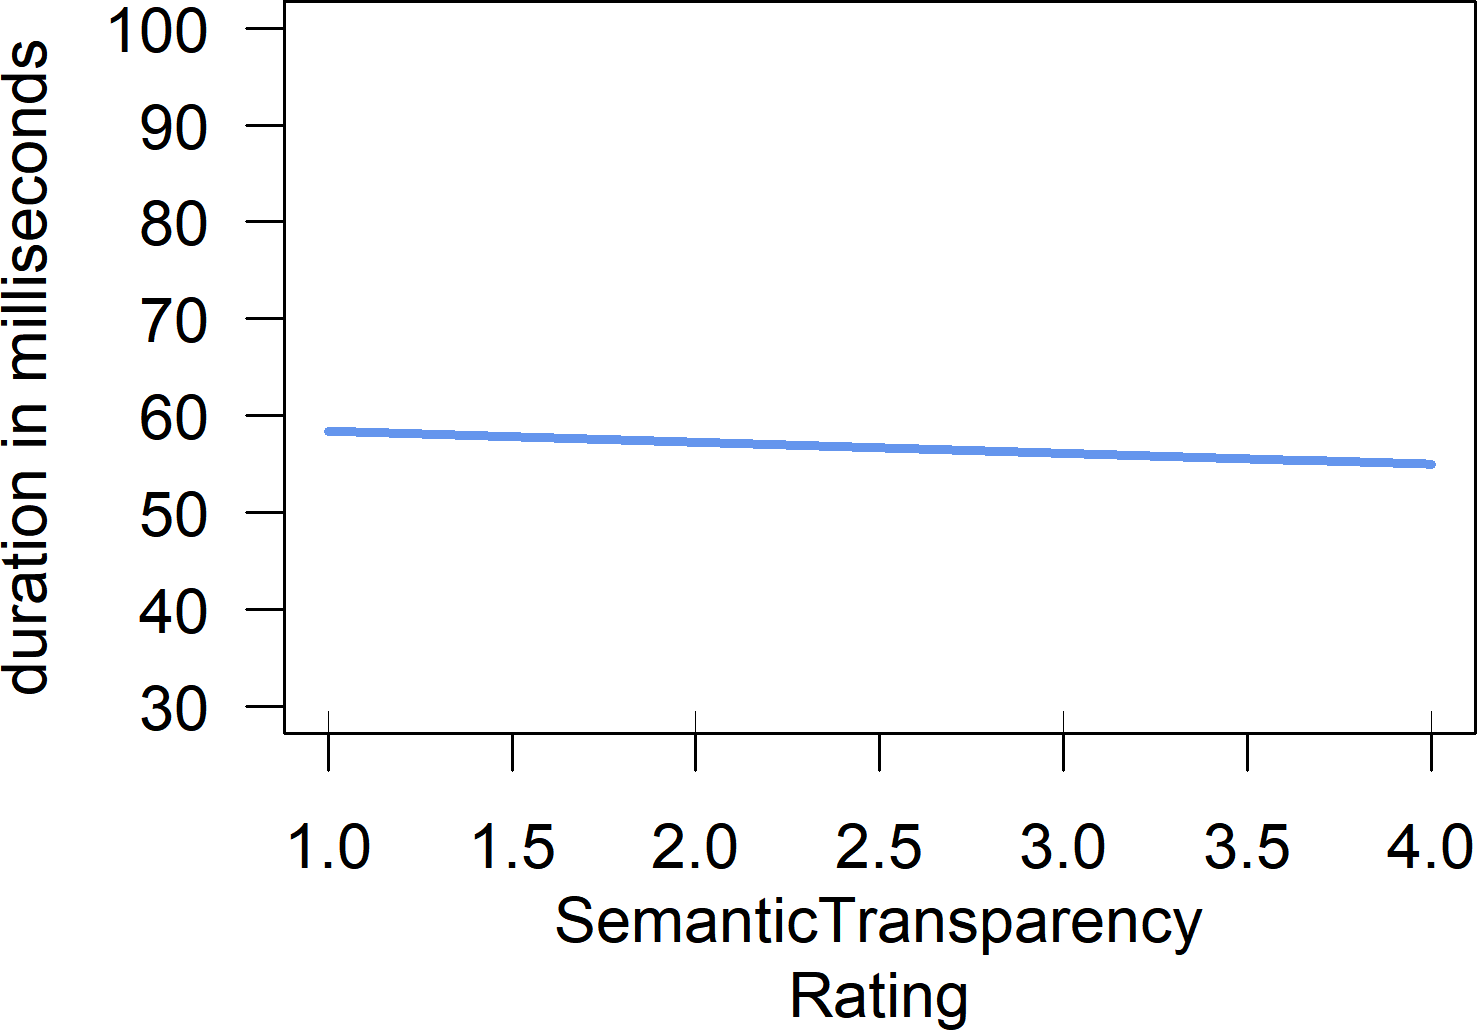
\includegraphics [scale=0.5] {images/Experiment/LyModelRating}
	\caption{Effect of semantic transparency rating on consonant duration in complex \suffix{ly}-data set}
	\label{fig: Rating  lyComplex experiment}

\end{figure*}





\begin{figure}
	
		
	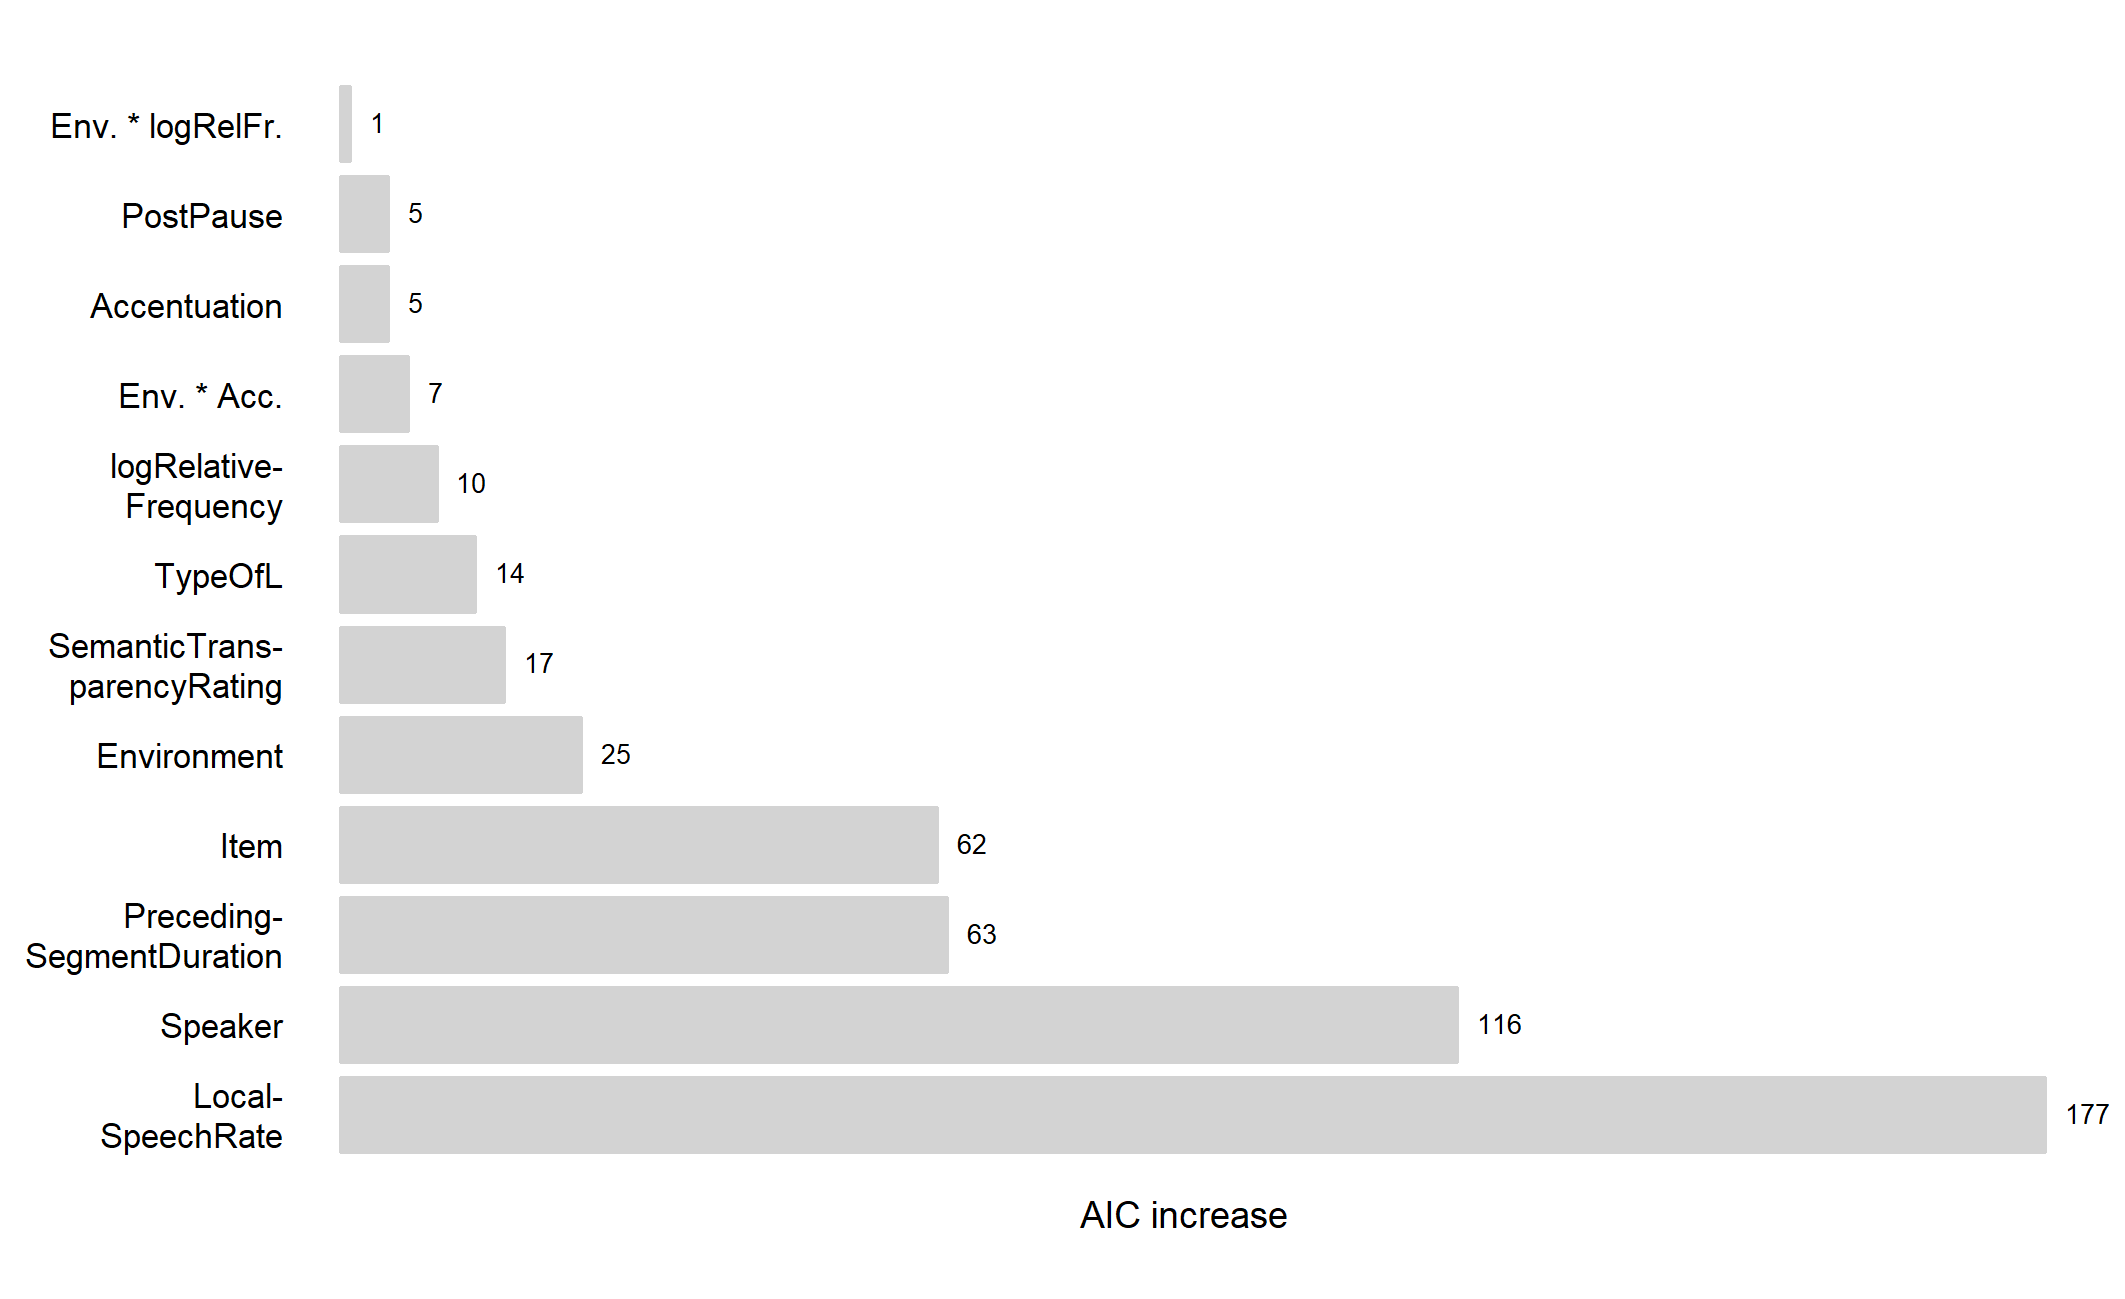
\includegraphics[scale=0.7]{images/Experiment/AICdecreaseLYComplex.png}
	\caption{AIC increase for each variable of the final \suffix{ly}-model, AIC final model = \textminus4915}
	\label{fig:Effect sozed ly compl Exp}

\end{figure}


The analysis of the AIC increase for each term in the model supports the analysis that \is{-ly}\suffix{ly} does not geminate. As can be seen in \figref{fig:Effect sozed ly compl Exp}, the AIC of the model increases by only 25 if the variable \textsc{Environment} is taken out of the model, i.e. the variable does not explain much of the variation in the model.
The figure furthermore shows that the \is{decomposability measure}decomposability measures do not explain much variance either. One should therefore be cautious to not over-interpret their effect. 
Most of the variance in the complex \is{-ly}\suffix{ly}-data is explained by noise variables, i.e. by \textsc{LocalSpeechRate}, \textsc{Speaker}, \textsc{PrecedingSegmentDuration} and \textsc{Item}. This fits in well with the corpus results. In the corpus study, all durational differences between \is{-ly}\suffix{ly}-suffixed words were explained by noise variables, i.e. no effect of \textsc{Environment} was found.




\subsubsection{Complete model}

The complex model suggests that \is{-ly}\suffix{ly} does not geminate. The complete model was fitted to provide some further evidence for this conclusion. Phonological doubles in words like \textit{really}, \textit{educationally} and \textit{solely} were compared to phonological singletons in simplex words which are represented by orthographic doubles, such as the /l/ in \textit{belly}, and to phonological singletons in base words, such as the /l/ in \textit{real}, \textit{educational} and \textit{sole}. 
If \is{-ly}\suffix{ly} does not geminate, as indicated by the complex model, phonological singletons in simplex words should be as long as phonological doubles. Furthermore, singletons in base words should be longer than double consonants. This is because word-final consonants are usually longer than word-internal consonants (see, for example,  \citealt{Berkovits.1993,Oller.1973,Umeda.1977}). 


The model with all \is{-ly}\suffix{ly}-words ($N=1645$) was fitted according to the modeling procedure described in \sectref{stats}. Due to an uneven distribution of the residuals in the initial model, the dependent variable \textsc{AbsoluteConsonantDuration} was Box-Cox-transformed ($\lambda = 0.061$) and 30 outliers were removed (1.82\% of the data).
After the model was refitted with the transformed dependent variable, it showed a satisfactory distribution of residuals.  The model was then simplified and interactions were tested (see \hyperref[Appendix G Summaries of tested interactions in experimental study]{Appendix G} for a list of all tested interactions).



The final model features seven variables: \textsc{Environment}, log\textsc{WordFormFre-quency},  \textsc{LocalSpeechRate}, \textsc{TypeOfL}, \textsc{PostPause}, \textsc{Accentuation} and \textsc{PrecedingSegmentDuration}. 
There are two interactions in the model, one between \textsc{Environment} and \textsc{PostPause}, and one between \textsc{Environment} and \textsc{Accentuation}. The final model is summarized in \tabref{model ly complete experiment} in \hyperref[Appendix H: Model Summaries Experiment]{Appendix H}.


The noise variables \textsc{LocalSpeechRate}, \textsc{TypeOfL}, and \textsc{PrecedingSegmentDuration} behave as expected. The higher the \isi{speech rate}, the shorter the lateral. A tap /l/ is shorter than an approximant /l/. And, the duration of the lateral becomes shorter when the duration of the preceding segment increases.
The variable log\textsc{WordFormFrequency} is only marginally significant in the model but shows the expected effect: with increasing \isi{frequency}, the lateral becomes shorter. 


\figref{fig:Env Acc ly Complete experiment} shows the effect of \textsc{Accentuation} by \textsc{Environment}. For each environment, the predicted consonant duration for items in \is{accentuation}accented position is indicated by light blue lines, and the predicted consonant duration for  items in unaccented position is indicated by dark blue lines.
 For convenience, the estimates for the four different structures, i.e. phonological singletons in complex words (\texttt{\#l-<l>}), phonological doubles in complex words  (\texttt{l\#l-<lel>}, \texttt{l\#l-<ll>}, \texttt{syll.l\#l-<ll>}), phonological singletons in base words (\texttt{l\#-<le>}, \texttt{l\#-<l>}, \texttt{syll. l\#-<ll>}), and phonological singletons in simplex words (\texttt{l-<l>}), are separated by vertical lines in the figure. 


\begin{figure*}
	

	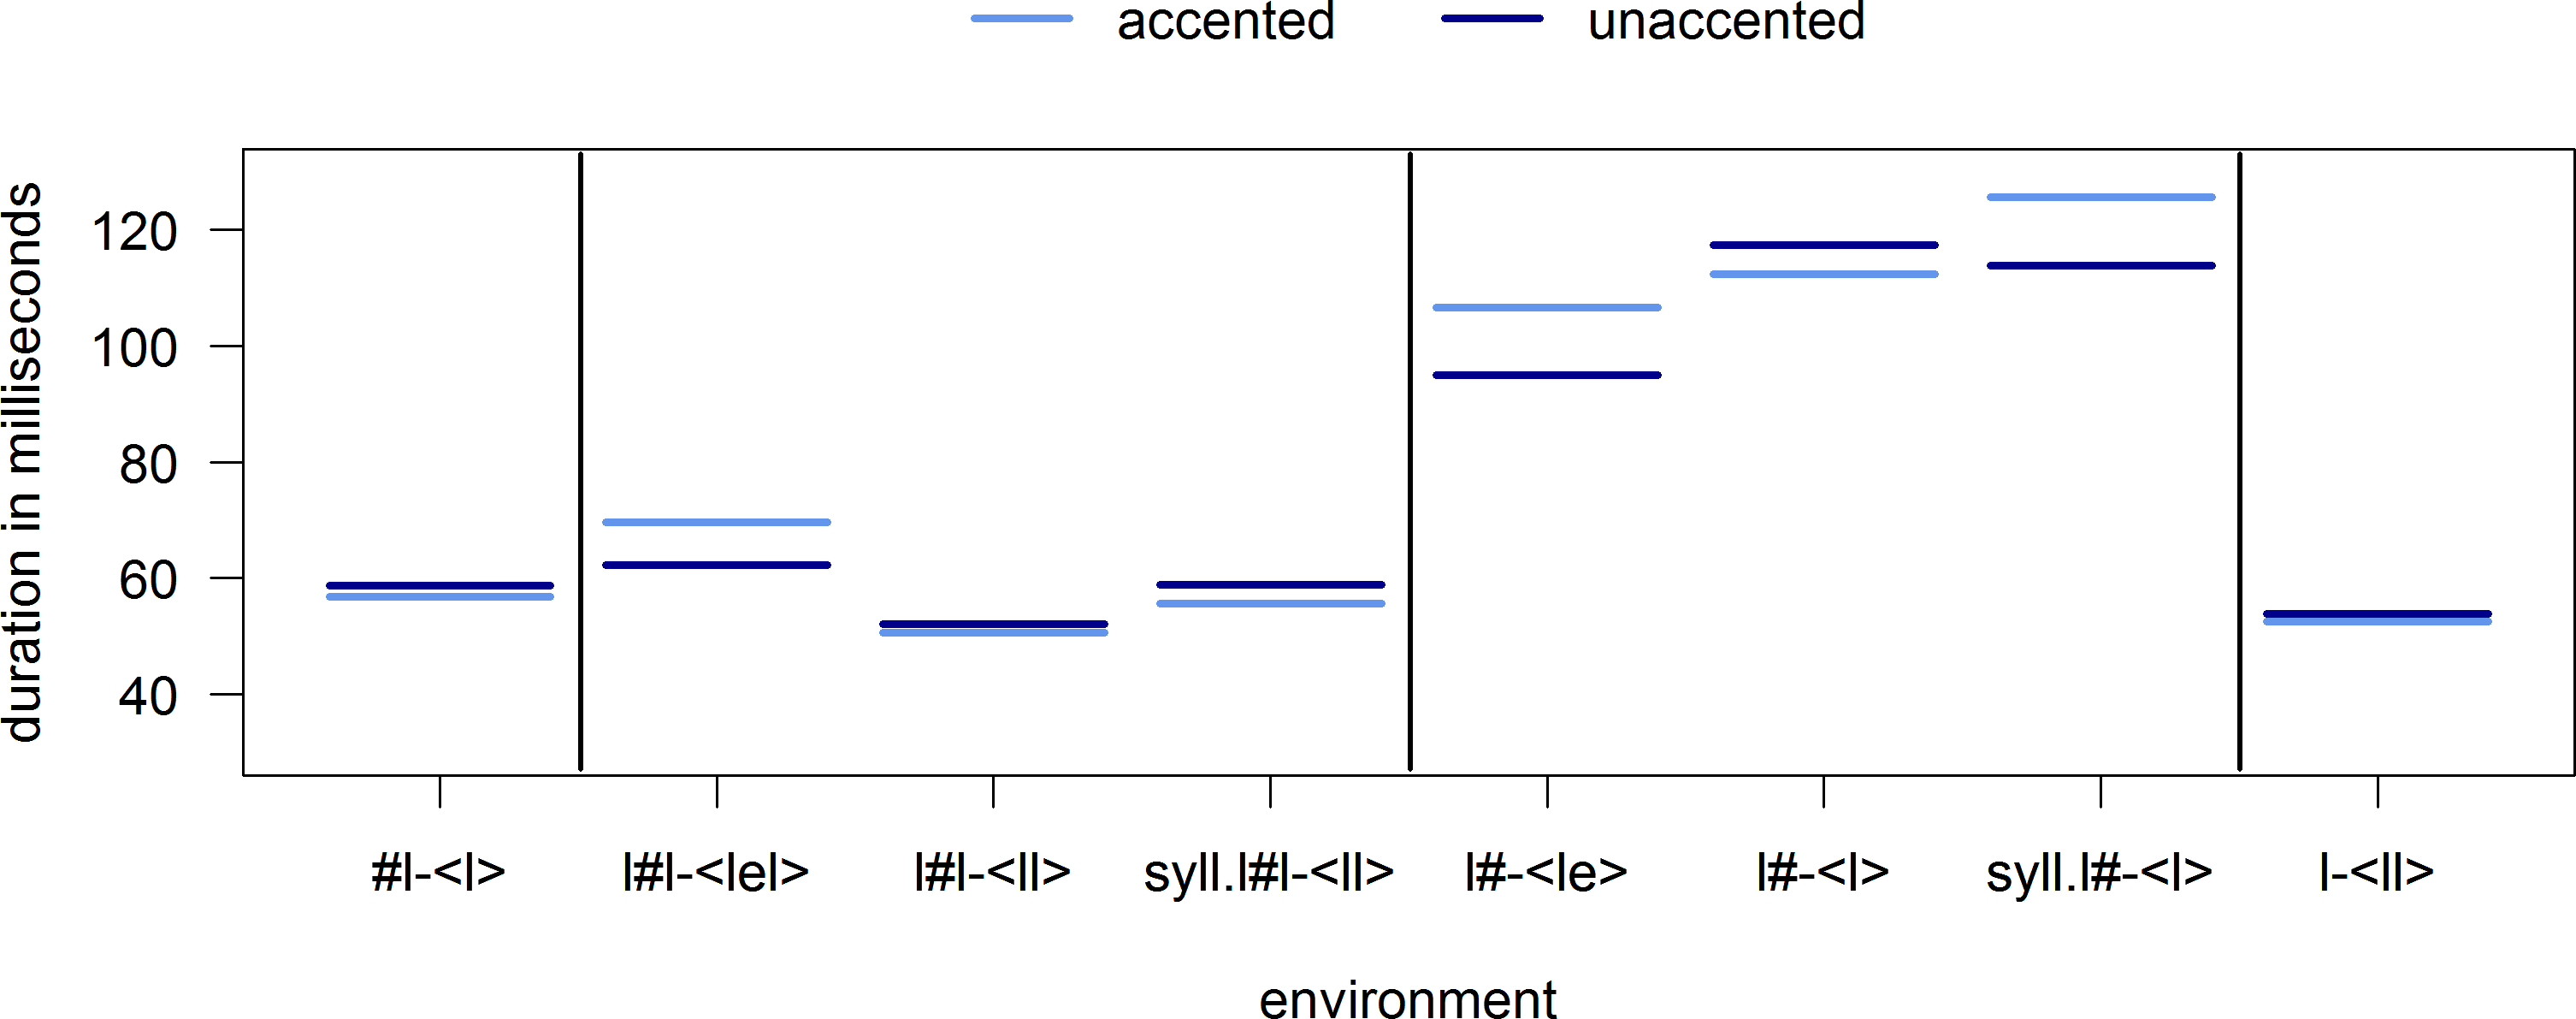
\includegraphics [scale=0.48] {images/Experiment/LyModelCompleteInterEnvAccLines}

	\caption{Effect of accentuation by environment on consonant duration in complete \suffix{ly}-data set}
	\label{fig:Env Acc ly Complete experiment}

\end{figure*}




 The figure shows the expected pattern. The durational differences between singletons in complex words and doubles in complex words resemble the ones of the complex model (cf. \figref{fig:Env Acc lyComplex experiment} in the previous section).\largerpage
 Furthermore, the laterals in base words are predicted to be longer than the laterals in all other environments. This is independent of \isi{accentuation}. 
 As expected, singletons in simplex words pattern with the phonological doubles: they are predicted to be slightly shorter than doubles of the \texttt{l\#l-<lel>}-environment, slightly longer than doubles of the \texttt{l\#l-<ll>}-environment, and as long as \is{syllabicity}syllabic doubles (\texttt{syll.l\#-<l>}). This is independent of \isi{accentuation}.
 
 
 
 \figref{fig:Env pause lyComplete experiment} shows the effect of \textsc{PostPause} by \textsc{Environment}. For each environment, the predicted consonant duration for items without a following pause is indicated by light blue lines, and the predicted consonant duration for  items with a following pause is indicated by dark blue lines.

 \begin{figure*}
 	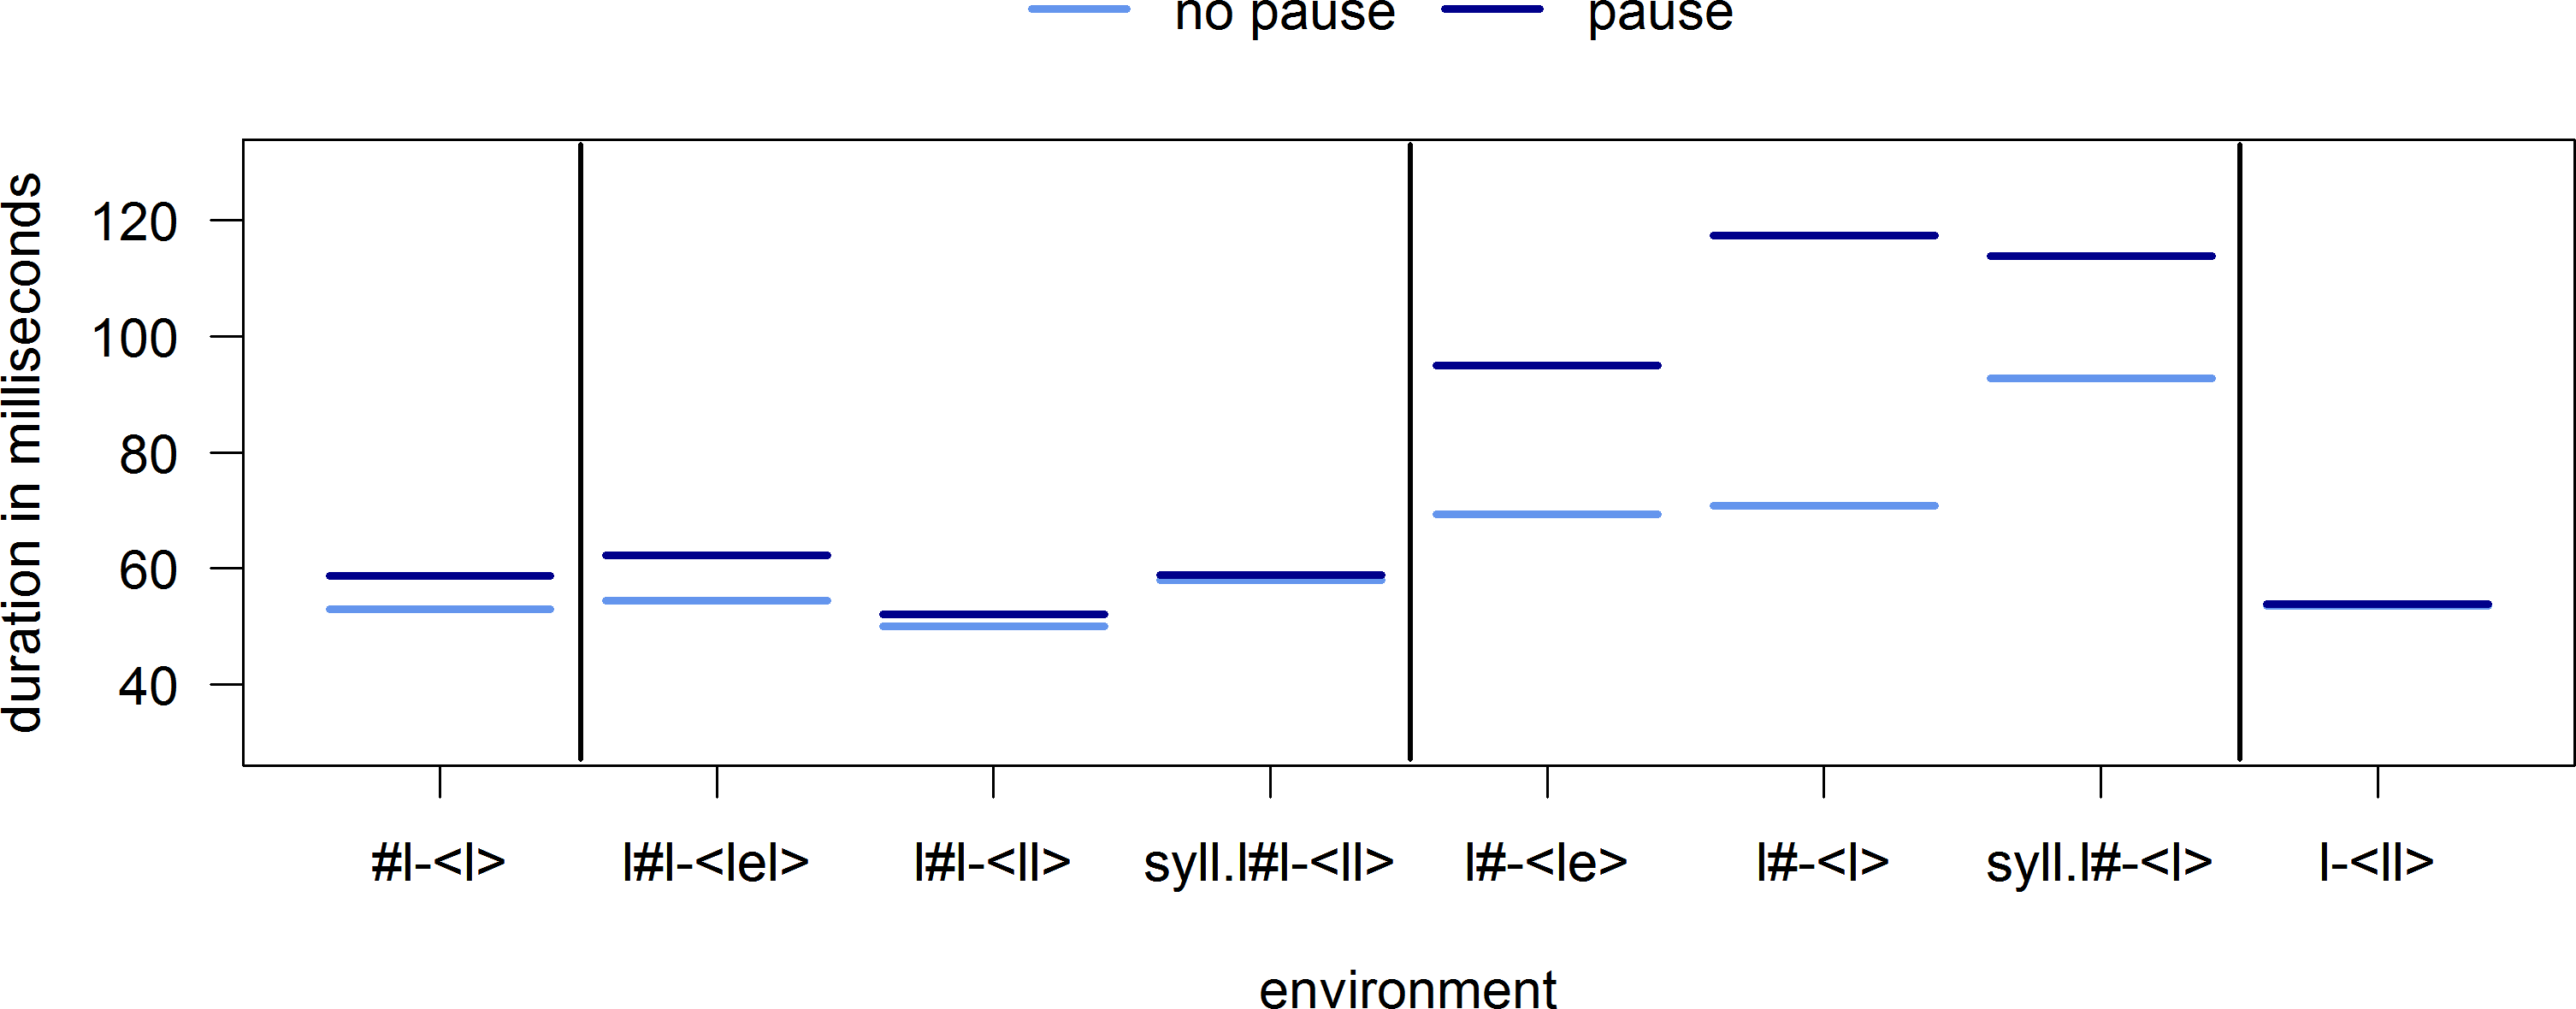
\includegraphics [scale=0.48] {images/Experiment/LyModelCompleteInterEnvPauseLines}
 	\caption{Effect of  post pause by environment on consonant duration in complete \suffix{ly}-data set}
 	\label{fig:Env pause lyComplete experiment}
 \end{figure*}
 

 Overall, the figure shows that same durational pattern as \figref{fig:Env Acc lyComplex experiment}. The three base environments (\texttt{l\#-<l>}, \texttt{syll.l\#-<l>}, \texttt{l\#-<le>}) clearly feature the longest lateral, and there are only minor durational differences between the lateral durations of the other environments. 
 With a following pause, the base-final /l/ becomes even longer, and the durational differences between the base-environ\-ments and all other environments increase. As only in base words /l/ is immediately followed by the pause, this is expected. 



To sum up, the complete model has supported the result of the complex model. The suffix \is{-ly}\suffix{ly} does not geminate. The double consonant is shorter than the word-final consonant in base words, and about as long as the singleton /l/ represented by an orthographic double. There is thus no indication that two underlying /l/s in \is{-ly}\suffix{ly}-suffixed words are realized with a longer duration than one underlying /l/.




\subsubsection{Summary} \label{ly experiment summary}\largerpage

In both \is{-ly}\suffix{ly}-models, the noise variables \textsc{Accentuation}, \textsc{LocalSpeechRate}, \textsc{PrecedingSegmentDuration}, \textsc{TypeOfL} and \textsc{PostPause} have shown expected effects. Additionally, in the complete model, the variable log\textsc{WordFormFrequency} affected consonant duration in the expected direction.

Both models have revealed that phonological doubles in \is{-ly}\suffix{ly}-suffixed words are not systematically longer than phonological singletons. Only under certain conditions, are some types of phonological double consonants, i.e. \is{syllabicity}syllabic ones and phonological doubles represented by the orthographic string $\langle$lel$\rangle$, longer than some types of phonological singletons. The longer duration of the doubles in those cases can be attributed to their \isi{syllabicity} and their \isi{orthography}, not to the fact that they feature two underlying consonants. 
One can conclude that the suffix \is{-ly}\suffix{ly} degeminates, and that \isi{syllabicity} and \isi{orthography} affect the \isi{acoustic realization} of /l/ in \is{-ly}\suffix{ly}-suffixed words. 

The complex model revealed effects of \isi{decomposability} with \is{-ly}\suffix{ly}. Items which were rated as less decomposable were produced with shorter consonant durations. Furthermore, for the \is{syllabicity}syllabic double consonants, \isi{relative frequency} affected consonant duration. With a higher \isi{relative frequency}, i.e. with less decomposable words, the consonant becomes shorter. 
These effects are in line with the assumption that less decomposable units are reduced, while more decomposable units are not reduced. However, the effect sizes are quite small and the effect of \isi{relative frequency} might be caused by just a few types in the data set. 

It is important to note that \isi{gemination} with \is{-ly}\suffix{ly} does not depend on \isi{relative frequency}. In other words, it is not the case that words with high \isi{relative frequency} degeminate and words with low \isi{relative frequency} geminate, or vice versa. If that was the case, \isi{relative frequency} would be significant for all double consonant environments. This is not the case. The effect of \isi{relative frequency} is independent of \isi{gemination}. 


\subsection{Summary} \label{discussion experiment}

% Categorical phenomenon
The first durational analyses looked at the distribution of duration across environments to get a first impression of whether the affixes under investigation geminate, and if so, whether \isi{gemination} is a gradient or a categorical phenomenon. 
For all affixes,  the analysis revealed that if there is a durational difference between doubles and singletons, durations are bimodally distributed with the doubles being longer than the singletons. As discussed in \sectref{predictions nature of gemination} (\textit{Nature of {gemination}: Predictions}), this indicates that \isi{gemination} is a categorical phenomenon.

% Models
For all data sets two or more linear models were fitted. One model predicted consonant duration with only complex words, and one model predicted consonant duration with all words of the data set, i.e. complex words, base words and simplex words with an orthographic double. 
Both models revealed very similar results, i.e. for the most part the same variables are significant in both models.
\tabref{tbl: Overview of complete results in the experimental study} shows an overview of the variables which show significant effects on \is{absolute duration}absolute consonant duration in the subsets. Only variables which are significant in at least one of the models, as independent effects or as part of an interaction, are listed. 



\begin{table*}
	\caption{Overview of significant variables in experimental models\label{tbl: Overview of complete results in the experimental study}}
	\begin{tabular} {lcclccc}
			\lsptoprule
			Variable & \textit{un-} & \textit{in-} & \textit{im-} & \textit{un-} \& \textit{in-} & \textit{dis-} & \textit{-ly}\\
			\midrule			
			\textsc{Environment}& \checkmark & \checkmark  & \checkmark  &\checkmark   &  \checkmark & \checkmark \\ 
			\textsc{Affix }&- &n.s. & n.s. & \checkmark  &-- & --\\ 
			\textsc{SemanticTransparencyRating}&n.s.& n.s.&n.s.  & -- &n.s. &\checkmark  \\
			log\textsc{RelativeFrequency}&n.s.& n.s.&n.s.  & -- &n.s. &\checkmark  \\
					\textsc{PC4}&--& --&\checkmark & -- &-- &--  \\	
			\textsc{LocalSpeechRate}&\checkmark & \checkmark & \checkmark & \checkmark  &\checkmark  & \checkmark \\	
			\textsc{Accentuation}&\checkmark &  \checkmark & \checkmark &\checkmark  & \checkmark & \checkmark \\		
			\textsc{PrePause}&\checkmark &\checkmark& \checkmark&\checkmark  & \checkmark & n.s.\\
			\textsc{BaseInitialStress}&\checkmark& \checkmark &\checkmark  & n.s. &-- &--\\
			
			\textsc{PrecedingSegmentDuration}&\checkmark &\checkmark & n.s. & n.s.&n.s.  & \checkmark \\

			\textsc{GlobalSpeechRate}&n.s.& n.s. &\checkmark  &n.s. &  n.s. & n.s.\\	

			\textsc{PostPause}&n.s. & n.s.& n.s. &n.s.  & n.s. &\checkmark \\		
			log\textsc{WordFormFrequency}&n.s. & n.s.& n.s. &n.s.  & n.s. &\checkmark \\		
						\textsc{TypeOfL}&-- & --& --&-- & --&\checkmark \\
			\midrule
		\multicolumn{6}{l}{\begin{tabular}{ll}
			\checkmark & significant in at least one of the models \\			
			n.s. & not significant in the models \\			
			--  & not included in the models \\
			\end{tabular}}\\
			\lspbottomrule
        \end{tabular}
\end{table*}




Overall, the noise variables showed the expected effects in all models. As can be seen in the table, the variables \textsc{LocalSpeechRate} and \textsc{Accentuation} are significant with all affixes. 
Some variables, such as \textsc{PrePause}, only affect consonant duration with the prefixes, and some, such as \textsc{PostPause}, only affect consonant duration with the suffix \is{-ly}\suffix{ly}.  
 Furthermore, there are some noise variables which only affect consonant duration in a few models, such as the variable \textsc{GlobalSpeechRate} or the variable \textsc{PrecedingSegmentDuration}. 

With regard to the variables of interest, three of the \is{decomposability measure}decomposability variables proved to be significant in the models: \textsc{PC4} for \is{im-}/ɪm/, and \textsc{SemanticTransparen- cyRating} and log\textsc{RelativeFrequency} for \is{-ly}\suffix{ly}. 
 All effects are, however, quite weak and do not allow for general conclusions about the effect of \isi{decomposability}. 
 
 As discussed in \sectref{in experiment}, the effect of \textsc{PC4} in the \is{im-}/ɪm/ -model is very weak and caused by only a few types with a particular feature combination. The effect is therefore not clearly interpretable in terms of \isi{decomposability}. 
 For \is{-ly}\suffix{ly}, the two \is{decomposability measure}decomposability variables \textsc{SemanticTransparencyRating} and log\textsc{RelativeFr\-equency} indicate that with increasing \isi{decomposability}, /l/ in \is{-ly}\suffix{ly}-suffixed words becomes longer. This is in line with the assumption that less decomposable units are reduced, while more decomposable units are not reduced. However, the effect sizes are quite small and the effect of \isi{relative frequency} is only significant for one environment, i.e. \is{syllabicity}syllabic doubles. 
Furthermore, the effect might be caused by only two types in the data set.


%
The variable of interest \textsc{Environment} significantly affects consonant duration in all models. 
However, the effect of \textsc{Environment} does not indicate \isi{gemination} for all affixes. Only for the prefixes, phonological doubles are systematically longer than phonological singletons, i.e. only the prefixes geminate. Double consonants with \is{-ly}\suffix{ly} are not systematically longer than corresponding singletons. The suffix \is{-ly}\suffix{ly} degeminates.  


While all prefixes geminate, there are differences in the \isi{degree of gemination} between them. While the prefix \is{un-}\prefix{un} clearly and strongly geminates, the \isi{degree of gemination} is much weaker for the two \is{in-}\prefix{in}prefixes and for \is{dis-}\prefix{dis}. The weaker \isi{degree of gemination} is indicated by four aspects: first, durational differences between doubles and singletons are smaller for \is{in-}\prefix{in} and \is{dis-}\prefix{dis} than for \is{un-}\prefix{un}.\footnote{See \tabref{tbl: Overview of environment in the experimental study} in \hyperref[Appendix I: Predicted Durations Experiment]{Appendix I} for an overview of the predicted consonant durations of prefixed words in the experimental study.} Second, while the double consonant in \is{un-}\prefix{un}prefixed words is longer than all types of singletons, the double consonant in \is{in-}\prefix{in} and \is{dis-}\prefix{dis}prefixed words is not. For example, the double in \is{in-}\prefix{in} and \is{dis-}\prefix{dis}prefixed words is not longer than the singleton in base words. Third, the variable \textsc{Environment} explains much less of the variance found in the \is{in-}\prefix{in} and \is{dis-}\prefix{dis}data than in the \is{un-}\prefix{un}data. 
Fourth, while \isi{gemination} with \is{un-}\prefix{un} is independent of prosodic factors, \isi{gemination} with \is{in-}\prefix{in} depends on \isi{stress}. Only when the base-initial syllable of an \is{in-}\prefix{in}prefixed word is \is{stress}stressed, the word geminates. For \is{dis-}\prefix{dis}, an interaction between \textsc{BaseInitialStress} and \textsc{Environment} could not be tested because of the distribution of \isi{stress} in the data set. The experimental study did not feature a \is{dis-}\prefix{dis}prefixed word with an unstressed base-initial syllable and a phonological double.

It is important to note that, in contrast to the experimental study, the corpus study featured one \is{dis-}\prefix{dis}prefixed type with a phonological double and an unstressed base-initial syllable (\textit{dissolution}). Interestingly, this was the only type which degeminated. As discussed in \sectref{Summary Corpus Study}, it remained unclear whether the \is{degemination}de\-gemination of \textit{dissolution} was caused by type-specific factors, its unstressed base-initial syllable or its \isi{semantic opacity}.
Since the experimental study has shown that \isi{gemination} does not depend on \isi{semantic transparency}, i.e. that semantically opaque \is{dis-}\prefix{dis}prefixed words geminate,  it now seems plausible to assume that the \isi{degemination} of \textit{dissolution} was not  caused by its \isi{semantic opacity} but by its unstressed base-initial syllable. This means one could also assume that other \is{dis-}\prefix{dis}prefixed words with a double consonant and an unstressed base-initial syllable also degeminate. Due to the non-existence of additional relevant types, i.e. additional \is{dis-}\prefix{dis}prefixed words with a double consonant and an unstressed base-initial syllable, it is however impossible to further investigate the issue. 




Further evidence for the conclusion that \is{in-}\prefix{in} geminates to a lesser degree than \is{un-}\prefix{un} can be gleaned from the model which directly compared the prefixes. In this model, the variable \textsc{Affix} interacts with the variable \textsc{Environment}. 
While the singletons of all three prefixes (\is{un-}\prefix{un}, \is{locative in-}locative \prefix{in} and \is{negative in-}negative \prefix{in}) are of comparable length, there is a significant difference in the duration of double consonants between the prefixes. The affix \is{un-}\prefix{un} features the longest double nasal,  and the double nasal with \is{negative in-}negative \prefix{in} is longer than the one with \is{locative in-}locative \prefix{in}. This decline in duration resembles the decline in \isi{segmentability} of the affixes. The prefix \is{un-}\prefix{un} is the most segmentable affix of the three, followed by \is{negative in-}negative \prefix{in}, followed by \is{locative in-}locative \prefix{in}. However, as discussed in \sectref{in experiment}, the only type featuring a double consonant and \is{locative in-}locative \prefix{in} is also the only /ɪn/-prefixed item with a double consonant featuring an unstressed base-initial syllable. It is therefore possible that the difference in \isi{gemination} between locative and \is{negative in-}negative \prefix{in} is actually caused by a difference in prosodic structure. This explanation is especially plausible as the variable \textsc{Affix} is not significant in any of the \is{in-}\prefix{in}models, whereas the variable \textsc{BaseInitialStress} interacts with the variable \textsc{Environment} in all of the \is{in-}\prefix{in}models. 
One can thus state that there is a difference in the \isi{degree of gemination} between \is{un-}\prefix{un} and \is{in-}\prefix{in}, but that there is no difference in the \isi{degree of gemination} between locative and \is{negative in-}negative \prefix{in}.


The experimental study revealed one other important fact with regard to the nature of \isi{gemination}. Gemination does not depend on \isi{orthography}. As evidenced by the complete \is{dis-}\prefix{dis} and \is{-ly}\suffix{ly}-models, orthographic doubles in simplex words (e.g. \textit{dissertation}, \textit{belly}) are not longer than orthographic singletons. 
In the \is{dis-}\prefix{dis}model, it was furthermore revealed that orthographic doubles in simplex words are shorter than phonological doubles. 
Thus, the lengthening of phonological doubles is not caused by their \isi{orthography}. %, i.e. by the fact that they are spelled with two consonants. 
Gemination in English is caused by the presence of two identical phonological consonants, not by the presence of two identical orthographic consonants.

To summarize, in all models the noise variables showed the expected effects. Furthermore, effects of {word-specific decomposability} were found for \is{-ly}\suffix{ly}. 
With regard to \isi{gemination}, the experimental study revealed that the prefixes \is{un-}\prefix{un}, \is{in-}\prefix{in} and \is{dis-}\prefix{dis} geminate. The suffix \is{-ly}\suffix{ly} degeminates. 
The prefix \is{un-}\prefix{un} geminates to a higher degree than the two \is{in-}\prefix{in}prefixes and \is{dis-}\prefix{dis}. The pattern of \isi{gemination} in the experimental study thus resembles the \isi{segmentability} and \isi{informativeness} of the affixes (see \textit{Semantic Segmentability Hierarchy} in \tabref{fig:Segmentability hierarchies of  affixes repetition 3} in \sectref{Exp The Segmentability of the Affixes: A Comparison}). The most informative and segmentable affix \is{un-}\prefix{un} clearly geminates, the least informative and least segmentable affix \is{-ly}\suffix{ly} degeminates, and the other affixes geminate to a rather low degree. Gemination does not depend on spelling. 
